% Options for packages loaded elsewhere
\PassOptionsToPackage{unicode}{hyperref}
\PassOptionsToPackage{hyphens}{url}
%
\documentclass[
  11pt,
  a4paper,
]{scrbook}

\usepackage{amsmath,amssymb}
\usepackage{setspace}
\usepackage{iftex}
\ifPDFTeX
  \usepackage[T1]{fontenc}
  \usepackage[utf8]{inputenc}
  \usepackage{textcomp} % provide euro and other symbols
\else % if luatex or xetex
  \usepackage{unicode-math}
  \defaultfontfeatures{Scale=MatchLowercase}
  \defaultfontfeatures[\rmfamily]{Ligatures=TeX,Scale=1}
\fi
\usepackage{lmodern}
\ifPDFTeX\else  
    % xetex/luatex font selection
\fi
% Use upquote if available, for straight quotes in verbatim environments
\IfFileExists{upquote.sty}{\usepackage{upquote}}{}
\IfFileExists{microtype.sty}{% use microtype if available
  \usepackage[]{microtype}
  \UseMicrotypeSet[protrusion]{basicmath} % disable protrusion for tt fonts
}{}
\makeatletter
\@ifundefined{KOMAClassName}{% if non-KOMA class
  \IfFileExists{parskip.sty}{%
    \usepackage{parskip}
  }{% else
    \setlength{\parindent}{0pt}
    \setlength{\parskip}{6pt plus 2pt minus 1pt}}
}{% if KOMA class
  \KOMAoptions{parskip=half}}
\makeatother
\usepackage{xcolor}
\usepackage[textheight=9in,,textwidth=6.5in,,top=1in,,headheight=14pt,,headsep=25pt,,footskip=30pt]{geometry}
\setlength{\emergencystretch}{3em} % prevent overfull lines
\setcounter{secnumdepth}{2}
% Make \paragraph and \subparagraph free-standing
\makeatletter
\ifx\paragraph\undefined\else
  \let\oldparagraph\paragraph
  \renewcommand{\paragraph}{
    \@ifstar
      \xxxParagraphStar
      \xxxParagraphNoStar
  }
  \newcommand{\xxxParagraphStar}[1]{\oldparagraph*{#1}\mbox{}}
  \newcommand{\xxxParagraphNoStar}[1]{\oldparagraph{#1}\mbox{}}
\fi
\ifx\subparagraph\undefined\else
  \let\oldsubparagraph\subparagraph
  \renewcommand{\subparagraph}{
    \@ifstar
      \xxxSubParagraphStar
      \xxxSubParagraphNoStar
  }
  \newcommand{\xxxSubParagraphStar}[1]{\oldsubparagraph*{#1}\mbox{}}
  \newcommand{\xxxSubParagraphNoStar}[1]{\oldsubparagraph{#1}\mbox{}}
\fi
\makeatother

\usepackage{color}
\usepackage{fancyvrb}
\newcommand{\VerbBar}{|}
\newcommand{\VERB}{\Verb[commandchars=\\\{\}]}
\DefineVerbatimEnvironment{Highlighting}{Verbatim}{commandchars=\\\{\}}
% Add ',fontsize=\small' for more characters per line
\usepackage{framed}
\definecolor{shadecolor}{RGB}{255,255,255}
\newenvironment{Shaded}{\begin{snugshade}}{\end{snugshade}}
\newcommand{\AlertTok}[1]{\textcolor[rgb]{0.75,0.01,0.01}{\textbf{\colorbox[rgb]{0.97,0.90,0.90}{#1}}}}
\newcommand{\AnnotationTok}[1]{\textcolor[rgb]{0.79,0.38,0.79}{#1}}
\newcommand{\AttributeTok}[1]{\textcolor[rgb]{0.00,0.34,0.68}{#1}}
\newcommand{\BaseNTok}[1]{\textcolor[rgb]{0.69,0.50,0.00}{#1}}
\newcommand{\BuiltInTok}[1]{\textcolor[rgb]{0.39,0.29,0.61}{\textbf{#1}}}
\newcommand{\CharTok}[1]{\textcolor[rgb]{0.57,0.30,0.62}{#1}}
\newcommand{\CommentTok}[1]{\textcolor[rgb]{0.54,0.53,0.53}{#1}}
\newcommand{\CommentVarTok}[1]{\textcolor[rgb]{0.00,0.58,1.00}{#1}}
\newcommand{\ConstantTok}[1]{\textcolor[rgb]{0.67,0.33,0.00}{#1}}
\newcommand{\ControlFlowTok}[1]{\textcolor[rgb]{0.12,0.11,0.11}{\textbf{#1}}}
\newcommand{\DataTypeTok}[1]{\textcolor[rgb]{0.00,0.34,0.68}{#1}}
\newcommand{\DecValTok}[1]{\textcolor[rgb]{0.69,0.50,0.00}{#1}}
\newcommand{\DocumentationTok}[1]{\textcolor[rgb]{0.38,0.47,0.50}{#1}}
\newcommand{\ErrorTok}[1]{\textcolor[rgb]{0.75,0.01,0.01}{\underline{#1}}}
\newcommand{\ExtensionTok}[1]{\textcolor[rgb]{0.00,0.58,1.00}{\textbf{#1}}}
\newcommand{\FloatTok}[1]{\textcolor[rgb]{0.69,0.50,0.00}{#1}}
\newcommand{\FunctionTok}[1]{\textcolor[rgb]{0.39,0.29,0.61}{#1}}
\newcommand{\ImportTok}[1]{\textcolor[rgb]{1.00,0.33,0.00}{#1}}
\newcommand{\InformationTok}[1]{\textcolor[rgb]{0.69,0.50,0.00}{#1}}
\newcommand{\KeywordTok}[1]{\textcolor[rgb]{0.12,0.11,0.11}{\textbf{#1}}}
\newcommand{\NormalTok}[1]{\textcolor[rgb]{0.12,0.11,0.11}{#1}}
\newcommand{\OperatorTok}[1]{\textcolor[rgb]{0.12,0.11,0.11}{#1}}
\newcommand{\OtherTok}[1]{\textcolor[rgb]{0.00,0.43,0.16}{#1}}
\newcommand{\PreprocessorTok}[1]{\textcolor[rgb]{0.00,0.43,0.16}{#1}}
\newcommand{\RegionMarkerTok}[1]{\textcolor[rgb]{0.00,0.34,0.68}{\colorbox[rgb]{0.88,0.91,0.97}{#1}}}
\newcommand{\SpecialCharTok}[1]{\textcolor[rgb]{0.24,0.68,0.91}{#1}}
\newcommand{\SpecialStringTok}[1]{\textcolor[rgb]{1.00,0.33,0.00}{#1}}
\newcommand{\StringTok}[1]{\textcolor[rgb]{0.75,0.01,0.01}{#1}}
\newcommand{\VariableTok}[1]{\textcolor[rgb]{0.00,0.34,0.68}{#1}}
\newcommand{\VerbatimStringTok}[1]{\textcolor[rgb]{0.75,0.01,0.01}{#1}}
\newcommand{\WarningTok}[1]{\textcolor[rgb]{0.75,0.01,0.01}{#1}}

\providecommand{\tightlist}{%
  \setlength{\itemsep}{0pt}\setlength{\parskip}{0pt}}\usepackage{longtable,booktabs,array}
\usepackage{calc} % for calculating minipage widths
% Correct order of tables after \paragraph or \subparagraph
\usepackage{etoolbox}
\makeatletter
\patchcmd\longtable{\par}{\if@noskipsec\mbox{}\fi\par}{}{}
\makeatother
% Allow footnotes in longtable head/foot
\IfFileExists{footnotehyper.sty}{\usepackage{footnotehyper}}{\usepackage{footnote}}
\makesavenoteenv{longtable}
\usepackage{graphicx}
\makeatletter
\newsavebox\pandoc@box
\newcommand*\pandocbounded[1]{% scales image to fit in text height/width
  \sbox\pandoc@box{#1}%
  \Gscale@div\@tempa{\textheight}{\dimexpr\ht\pandoc@box+\dp\pandoc@box\relax}%
  \Gscale@div\@tempb{\linewidth}{\wd\pandoc@box}%
  \ifdim\@tempb\p@<\@tempa\p@\let\@tempa\@tempb\fi% select the smaller of both
  \ifdim\@tempa\p@<\p@\scalebox{\@tempa}{\usebox\pandoc@box}%
  \else\usebox{\pandoc@box}%
  \fi%
}
% Set default figure placement to htbp
\def\fps@figure{htbp}
\makeatother
% definitions for citeproc citations
\NewDocumentCommand\citeproctext{}{}
\NewDocumentCommand\citeproc{mm}{%
  \begingroup\def\citeproctext{#2}\cite{#1}\endgroup}
\makeatletter
 % allow citations to break across lines
 \let\@cite@ofmt\@firstofone
 % avoid brackets around text for \cite:
 \def\@biblabel#1{}
 \def\@cite#1#2{{#1\if@tempswa , #2\fi}}
\makeatother
\newlength{\cslhangindent}
\setlength{\cslhangindent}{1.5em}
\newlength{\csllabelwidth}
\setlength{\csllabelwidth}{3em}
\newenvironment{CSLReferences}[2] % #1 hanging-indent, #2 entry-spacing
 {\begin{list}{}{%
  \setlength{\itemindent}{0pt}
  \setlength{\leftmargin}{0pt}
  \setlength{\parsep}{0pt}
  % turn on hanging indent if param 1 is 1
  \ifodd #1
   \setlength{\leftmargin}{\cslhangindent}
   \setlength{\itemindent}{-1\cslhangindent}
  \fi
  % set entry spacing
  \setlength{\itemsep}{#2\baselineskip}}}
 {\end{list}}
\usepackage{calc}
\newcommand{\CSLBlock}[1]{\hfill\break\parbox[t]{\linewidth}{\strut\ignorespaces#1\strut}}
\newcommand{\CSLLeftMargin}[1]{\parbox[t]{\csllabelwidth}{\strut#1\strut}}
\newcommand{\CSLRightInline}[1]{\parbox[t]{\linewidth - \csllabelwidth}{\strut#1\strut}}
\newcommand{\CSLIndent}[1]{\hspace{\cslhangindent}#1}

% Palatino font:
\usepackage[T1]{fontenc}
\usepackage[utf8]{inputenc}

% For the abstract
\usepackage{ragged2e}

% Add new fonts 
\usepackage{newpxtext}
\usepackage{newpxmath}


% % Palatino and math font to match
% \usepackage{palatino}
% \usepackage{mathpazo}

\usepackage{upquote}

% % front page
% \usepackage[colorlinks]{hyperref} % for text color on title
% \usepackage{titling} % makes \thetitle etc available...
% \usepackage{lipsum}
% \usepackage{tikz}
% \tikzstyle{bag} = [align=center] % allows new lines in text below
% \AtBeginDocument{\thispagestyle{empty}
% \definecolor{titlecolor}{HTML}{1C2404}
% \begin{tikzpicture}[remember picture,overlay]
% \draw (current page.center) node[inner sep=0, opacity=0.5] {\resizebox{!}{350mm}{\includegraphics{highres_banner.pdf}}};
% \draw (current page.center) node[inner sep=0, opacity=0.5] {\resizebox{!}{100mm}{
\includegraphics{ausegl_sort.pdf}}};
% % \draw (current page.center) node[bag] {  
%         \draw (17, 1.7) node[bag, align=right, anchor=north east] {  
%     % \mytitlefont 
%     \color{titlecolor} \Large \textbf{Master's Thesis in Bioinformatics} \\ 
%     \\ 
%     % \mytitlefont 
%     \color{titlecolor} \Huge \textbf{\thetitle} \\ 
%     \\ 
%     % \mytitlefont
%     \color{titlecolor} \huge \theauthor \\
%     \\
%     % \mytitlefont 
%     \color{titlecolor} \Large \thedate 
%     };
% \end{tikzpicture}
% \clearpage}

% % back side
% \AtEndDocument{\clearpage\thispagestyle{empty}
% \begin{tikzpicture}[remember picture,overlay]
% \draw (current page.center) node[inner sep=0, opacity=0.5] {\resizebox{!}{350mm}{\includegraphics{highres_banner.pdf}}};
% % \draw (current page.center) node[bag] {  
%     \draw (17, 1.7) node[bag, align=right, anchor=north east] {  
%         % \mytitlefont 
%         \color{titlecolor} \large Bioinformatics Research Centre \\ 
%         % \mytitlefont 
%         \color{titlecolor} \large Department of Molecular Biology and Genetics \\ 
%         % \mytitlefont 
%         \color{titlecolor} \large Aarhus University \\
%         % \mytitlefont 
%         \color{titlecolor} \large Universitetsbyen 81 \\
%         % \mytitlefont 
%         \color{titlecolor} \large 8000 Aarhus C \\
%         % \mytitlefont 
%         \color{titlecolor} \large Denmark
%         };

% \end{tikzpicture}}


% % picture (AU logo in title page)
% \usepackage{titlepic}
% % \usepackage{graphicx}
% \titlepic{\resizebox{!}{50mm}{
\includegraphics[width=\textwidth]{ausegl_sort.pdf}}}



% \pagestyle{plain} % no running header

\usepackage[many]{tcolorbox}
\definecolor{quotegray}{HTML}{505050}
\newtcolorbox{myquote}{%
    enhanced jigsaw, 
    breakable,      % allow page breaks
    frame hidden,   % hide the default frame
    left=1cm,       % left margin
    right=1cm,      % right margin
    colback=white,
    fontupper=\color{quotegray},
    overlay={%
        \node [scale=4,
            text=lightgray,
            inner sep=0pt,] at ([xshift=0.5cm,yshift=-0.7cm]frame.north west){``}; 
        \node [scale=4,
            text=lightgray,
            inner sep=0pt,] at ([xshift=-0.5cm]frame.south east){''};  
            },
        % paragraph skips obeyed within tcolorbox
                parbox=false,
}
% redefine the 'quote' environment to use this 'myquote' environment
\renewenvironment{quote}{\begin{myquote}}{\end{myquote}}

% add a dummy abstract environment that is defined in quarto manuscript 
% but not in the quarto book that we run first to give it a slot in the 
% side bar
\ifcsmacro{abstract}{}{
  \let\endmyenvironment\undefined%
  \newenvironment{abstract}{\chapter*{Abstract}}{}
}

% \usepackage{framed} % not sure i need this anymore

% \usepackage[T1]{fontenc}
% \usepackage{inconsolata}

% % I have to only define Shaded if it is already defined.
% % The reason is that pandoc does not define the macro if there are not code blocks in the a markdown file.
% \ifx \@Shaded \@empty

% \renewcommand{\KeywordTok}[1]{\textcolor[rgb]{0, 0, 0}{\textbf{{#1}}}} % def and or not reg
% \renewcommand{\BuiltInTok}[1]{\textcolor[rgb]{0.373, 0.298, 0.580}{\textbf{{#1}}}} % print open 
% \renewcommand{\VariableTok}[1]{\textcolor[rgb]{0.141, 0.392, 0.824}{\textbf{{#1}}}}
% \renewcommand{\OperatorTok}[1]{\textcolor[rgb]{0, 0, 0}{{#1}}} % def and or not reg
% \renewcommand{\DataTypeTok}[1]{\textcolor[rgb]{1.0,0.13,0.00}{{#1}}}
% \renewcommand{\DecValTok}[1]{\textcolor[rgb]{0.655, 0.498, 0.161}{{#1}}}
% \renewcommand{\BaseNTok}[1]{\textcolor[rgb]{0.259, 0.592, 0.596}{{#1}}}
% \renewcommand{\FloatTok}[1]{\textcolor[rgb]{0.655, 0.498, 0.161}{{#1}}}
% \renewcommand{\CharTok}[1]{\textcolor[rgb]{0.678,0.141,0.098}{{#1}}}
% \renewcommand{\StringTok}[1]{\textcolor[rgb]{0.678,0.141,0.098}{{#1}}}
% \renewcommand{\CommentTok}[1]{\textcolor[rgb]{0.135, 0.134, 0.133}{{#1}}}
% \renewcommand{\OtherTok}[1]{\textcolor[rgb]{0.00,0.44,0.13}{{#1}}}
% \renewcommand{\AlertTok}[1]{\textcolor[rgb]{1.00,0.00,0.00}{\textbf{{#1}}}}
% \renewcommand{\FunctionTok}[1]{\textcolor[rgb]{0.549, 0.102, 0.063}{\textbf{{#1}}}}  % function name
% \renewcommand{\RegionMarkerTok}[1]{{#1}}
% \renewcommand{\ErrorTok}[1]{\textcolor[rgb]{1.00,0.00,0.00}{\textbf{{#1}}}}
% \renewcommand{\NormalTok}[1]{\textcolor[rgb]{0, 0, 0}{{#1}}}


% \else
%   % no code blocks with markup...
% \fi



\usepackage{etoolbox}
\makeatletter
\g@addto@macro{\appendix}{%
  \patchcmd{\@@makechapterhead}% <cmd>
    {\endgraf\nobreak\vskip.5\baselineskip}% <search>
    {\hspace*{-.5em}:\space}% <replace>
    {}{}% <success><failure>
  \patchcmd{\@chapter}% <cmd>
    {\addchaptertocentry{\thechapter}}% <search>
    {\addchaptertocentry{Appendix~\thechapter:}}% <replace>
    {}{}% <success><failure>
  \addtocontents{toc}{%
    \protect\patchcmd{\protect\l@chapter}% <cmd>
      {1.5em}% <search>
      {6.5em}% <replace>
      {}{}}% <success><failure>
}
\renewcommand{\autodot}{}% Remove all end-of-counter dots
\makeatother


% restart chapter numbers in each part
\makeatletter
\@addtoreset{chapter}{part}
\makeatother


% \usepackage{chngcntr}
% \counterwithin*{subsubsection}{chapter}
% \counterwithout*{subsubsection}{section}
% \counterwithout*{subsubsection}{subsection}

% %  % KMT only use subsubsection number (this increments though the book 
% %  % when we supress numbering with  {.unnumbered} after each header except Exerisices
% \renewcommand\thesubsubsection{\arabic{section}}
% \renewcommand\thesubsubsection{\arabic{subsection}}
% \renewcommand\thesubsubsection{\arabic{chapter}-\arabic{subsubsection}}


\renewcommand*{\chapterformat}{%
\textcolor[rgb]{0.7, 0.7, 0.7}{\thechapter}\autodot\enskip%
}
\renewcommand*{\sectionformat}{%
\textcolor[rgb]{0.7, 0.7, 0.7}{\thesection}\autodot\enskip%
}
\renewcommand*{\subsectionformat}{%
\textcolor[rgb]{0.7, 0.7, 0.7}{\thesubsection}\autodot\enskip%
}
\renewcommand*{\subsubsectionformat}{%
\textcolor[rgb]{0.7, 0.7, 0.7}{\thesubsubsection}\autodot\enskip%
}

% %% from arcxiv.sty:  %%%
\RedeclareSectionCommand[
  beforeskip=-2ex,
  afterskip=1.5ex
]{chapter}

\RedeclareSectionCommand[
  beforeskip=-1.8ex,
  afterskip=0.8ex
]{section}

\RedeclareSectionCommand[
  beforeskip=-1.5ex,
  afterskip=0.5ex
]{subsection}

\RedeclareSectionCommand[
  beforeskip=1.5ex,
  afterskip=-1em
]{subsubsection}

\RedeclareSectionCommand[
  beforeskip=1.5ex,
  afterskip=-1em
]{paragraph}

% \RedeclareSectionCommand[
%   beforeskip=1.5ex plus 0.5ex minus 0.2ex,
%   afterskip=-1em
% ]{subparagraph}


\setkomafont{section}{\normalfont\Large\bfseries\raggedright}
\setkomafont{subsection}{\normalfont\large\bfseries\raggedright}
\setkomafont{subsubsection}{\normalfont\normalsize\bfseries\raggedright}
\setkomafont{paragraph}{\normalfont\normalsize\bfseries}
\setkomafont{subparagraph}{\normalfont\normalsize\bfseries}

\setkomafont{caption}{\small}
\setkomafont{captionlabel}{\bfseries\sffamily}

%% Tables
% \usepackage[style=plaintop]{floatrow}
% \floatsetup[table]{capposition=top}
% \floatsetup[figure]{capposition=bottom}
% \floatsetup[table]{font=small}
% \usepackage{booktabs} % professional-quality tables (arxiv.sty)

\usepackage[font={footnotesize},labelfont={bf}]{caption}
\AddToHook{env/longtable/before}{\fontsize{9}{11}\selectfont}
\AddToHook{env/longtable/after}{\normalsize}
\AddToHook{env/table/before}{\fontsize{9}{11}\selectfont}
\AddToHook{env/table/after}{\normalsize}
\AddToHook{env/codelisting/before}{\fontsize{9}{11}\selectfont}
\AddToHook{env/codelisting/after}{\normalsize}
% \usepackage{caption}
\captionsetup[sub]{font=footnotesize,labelfont=footnotesize, position=top}
\captionsetup[codelisting]{font=footnotesize, labelfont=bf}
% \captionsetup[subtable]{font=scriptsize,labelfont=scriptsize, position=top}


%%% For code blocks using the Shaded environment
% \AddToHook{env/Shaded/before}{\vspace{-0.5em}\small} % Reduces space before
% \AddToHook{env/Shaded/after}{\vspace{-1em}} % Reduces space after
\definecolor{shadecolor}{RGB}{250,250,250}

\renewenvironment{Shaded}
{
  \vspace{-0.5em} % Add spacing before
  \begin{snugshade} % Begin shaded block
  \small % Smaller font
}
{
  \end{snugshade} % End shaded block
  \vspace{-1em} % Add spacing after
}

%%%


% prevent latex from "floating" the figures
\usepackage{float}
\let\origfigure\figure
\let\endorigfigure\endfigure
\renewenvironment{figure}[1][2] {
    \expandafter\origfigure\expandafter[htbp]
} {
    \endorigfigure
}

% \usepackage{xcolor}
% % \let\oldtextit\textit 
% % \renewcommand\textit[1]{\oldtextit{\color{blue}#1}}
% \let\oldemph\emph
% \renewcommand\emph[1]{\oldemph{\color{gray}#1}}

\makeatletter
\@ifpackageloaded{caption}{}{\usepackage{caption}}
\AtBeginDocument{%
\ifdefined\contentsname
  \renewcommand*\contentsname{Table of contents}
\else
  \newcommand\contentsname{Table of contents}
\fi
\ifdefined\listfigurename
  \renewcommand*\listfigurename{List of Figures}
\else
  \newcommand\listfigurename{List of Figures}
\fi
\ifdefined\listtablename
  \renewcommand*\listtablename{List of Tables}
\else
  \newcommand\listtablename{List of Tables}
\fi
\ifdefined\figurename
  \renewcommand*\figurename{Figure}
\else
  \newcommand\figurename{Figure}
\fi
\ifdefined\tablename
  \renewcommand*\tablename{Table}
\else
  \newcommand\tablename{Table}
\fi
}
\@ifpackageloaded{float}{}{\usepackage{float}}
\floatstyle{ruled}
\@ifundefined{c@chapter}{\newfloat{codelisting}{h}{lop}}{\newfloat{codelisting}{h}{lop}[chapter]}
\floatname{codelisting}{Listing}
\newcommand*\listoflistings{\listof{codelisting}{List of Listings}}
\makeatother
\makeatletter
\makeatother
\makeatletter
\@ifpackageloaded{caption}{}{\usepackage{caption}}
\@ifpackageloaded{subcaption}{}{\usepackage{subcaption}}
\makeatother

\usepackage{bookmark}

\IfFileExists{xurl.sty}{\usepackage{xurl}}{} % add URL line breaks if available
\urlstyle{same} % disable monospaced font for URLs
\hypersetup{
  pdftitle={Chromatin Compartments and Selection on X},
  pdfkeywords={Hi-C, Chromatin Compartments, Selection on X, Selfish
gene drive},
  hidelinks,
  pdfcreator={LaTeX via pandoc}}


\title{Chromatin Compartments and Selection on X}
\usepackage{etoolbox}
\makeatletter
\providecommand{\subtitle}[1]{% add subtitle to \maketitle
  \apptocmd{\@title}{\par {\large #1 \par}}{}{}
}
\makeatother
\subtitle{How Edges of Active Chromatin Align with Selection Regions in
Primates}
\author{Søren Jørgensen \and Kasper Munch}
\date{2025-01-15}

\begin{document}
\frontmatter
\cleardoublepage
\thispagestyle{empty}
{\centering
\hbox{}\vskip 0cm plus 1fill

{%\mytitlefont 
\Huge\bfseries Chromatin Compartments and Selection on X \par}
\vspace{3ex}
{\Large\bfseries How Edges of Active Chromatin Align with Selection
Regions in Primates \par}
\vspace{5ex}

        {\bfseries Author: \\ \vspace{0.5ex}}
        {\bfseries\Large Søren Jørgensen \\ \vspace{0.7ex}}
            {\large Student ID: 201906763 \\ \vspace{1.2ex} }
        %
        {\bfseries Supervisor: \\ \vspace{0.5ex}}
        {\bfseries\Large Kasper Munch \\ \vspace{0.7ex}}
        %
        \par \vspace{0.7ex}
        %
        {\large Bioinformatics Research Center (BiRC) \\ \vspace{0.7ex}}
        %
        %
        {\large Molecular Biology and Genetics \\ \vspace{0.7ex}}
        %
        {\large Aarhus University, Denmark \\ \vspace{2ex}}
    %
%
\vskip 0cm plus 2fill

{\resizebox{!}{50mm}{
\includegraphics[width=\textwidth]{hicausegl.pdf}} \par}
\vskip 0cm plus 2fill

{\bfseries\Large\textit{MSc. Bioinformatics} \par}
\vspace{3ex}

{\large 2025-01-15 \par}
\vspace{3ex}

\vspace{10ex}
{\small Submitted in fulfillment of the requirements
of the degree of MSc. Bioinformatics \par}
\pagebreak


\vspace*{\fill} % Push content to the vertical middle of the page
\noindent
\begin{minipage}{.8\textwidth}
    \centering
    \hspace*{\fill}\rule{0.5\textwidth}{0.4pt}\hspace*{\fill} % Centered horizontal line
    \par \vspace{2em} % Add some vertical space
    {\Large\bfseries\scshape Abstract} % Abstract title
    \par % End the paragraph
    \vspace{1em} % Add some vertical space below the title
    \justifying % Ensure the abstract text is justified (requires the `ragged2e` package)
    The X chromosome is uniquely exposed to selective pressures due to
the lack of a second copy in the hemizygous sex, leaving no buffer
against deleterious mutations, and giving unique inheritance patterns.
Combined with its high density of essential genes related to
reproduction and brain function, this suggests the presence of
biological mechanisms that safeguard the integrity of the X chromosome.

In this study, the 3D chromatin architecture of the X chromosome in
rhesus macaque (\emph{Macaca mulata}) is investigated in the context of
evolutionary pressures and genetic drivers. To ensure transparency and
reproducibility, we adopt a comprehensive computational framework for
publishing a version-controlled, fully reproducible analysis.

We compare two Hi-C analysis frameworks, \emph{HiCExplorer} and
\emph{cooler/cooltools} (Open2C), on a subset, finding Open2C to be most
flexible. The ICE method (Iterative Correction and Eigendecomposition)
was used to infer conventional and refined A/B compartments for
fibroblast and four stages of spermatogenesis.

We find 200 kbp transition-zones between A/B-compartments on the X
chromosomes in both fibroblasts and round spermatids that align well
with strong selective sweeps in humans (ECH-regions), but not with
strong negative selection in baboons (\emph{Papio} spp.). We find that
most edges either overlap or are in significant proximity of each other
when comparing regions under selection in human and baboons with
A/B-compartments inferred Hi-C matrices at 100kb resolution and
restricting eigendecomposition along the X chromosome to 10Mb windows.
We discuss the biological meaning of these findings, where conserved
chromatin features may help to retain non-advantageous alleles, hinting
to the role of structural features aiding in genome
evolution. % Insert the abstract text here
    \par % End the paragraph
    \vspace{2em} % Add vertical space
    \hspace*{\fill}\rule{0.5\textwidth}{0.4pt}\hspace*{\fill} % Centered horizontal line
\end{minipage}
\vspace*{\fill} % Push the remaining content to the bottom of the page

}
\renewcommand*\contentsname{Table of contents}
{
\setcounter{tocdepth}{2}
\tableofcontents
}

\setstretch{1.25}
\mainmatter
\chapter{Introduction}\label{introduction}

The X chromosome plays a unique role in evolution, being directly
exposed to selection pressures due to its hemizygosity in males, leading
to unique inheritance patterns. Regions of reduced diversity on the X
chromosome could reflect the influence of strong evolutionary forces
that are aided by structural features of the genome. Chromatin
architecture, particularly the organization into A/B compartments, may
provide insights into the functional basis of these patterns.

Here, I analyze the 3D chromatin structure of the X chromosome in rhesus
macaque (\emph{Macaca mulata}) using Hi-C data on the latest reference
genome (rheMac10). The analysis extensively combines software tools that
emphasize reproducibility, ensuring that the analyses are transparent,
portable, and replicable.

\section{Evolution on X}\label{evolution-on-x}

The production of gametes in a sexually reproducing organism is a highly
complex process that involves numeruous elements. Spermatogenesis, the
process of forming male gametes, involves four stages of differentiation
from a germ cell through \emph{spermatogonia}, \emph{pachytene
spermatocyte}, and \emph{round spermatids} to \emph{spermatozoa} (Wang
et al. 2019), and is the basis of male reproduction. The specialized
cell division of meiosis neatly handles the pairing, recombination, and
segregation of homologous chromosomes, thereby ensuring proper genetic
distribution. A thorough understanding of the molecular steps of
reproduction and how genetic material is inherited is essential in
biology, bringing insight to areas such as speciation, population
diversity, and infertility.

Sex chromosomes differ from autosomes in several ways, primarily due to
their unique inheritance patterns and copy number. The Y chromosome is
present only in males, with a single copy per individual. The X
chromosome, on the other hand, has a more complex inheritance pattern:
males have one copy, while females have two. As a result, X chromosomes
spend two-thirds of their time in females and only one-third in males.
This skewed ratio influences the dynamics of selection on the X
chromosome. Furthermore, in males, the single-copy nature of the X
chromosome (hemizygosity) means that any mutations or loss of function
are directly exposed, as there is no second copy to compensate. This
concept also underpins Haldane's rule (Haldane 1922), which states that
in hybrids of two species, the heterogametic sex (e.g., XY in mammals,
ZW in birds) is the first to exhibit reduced fitness, such as sterility,
or to disappear entirely. Even a century later, the exact reasons for
this phenomenon remain debated, with several hypotheses proposed. These
include:

\begin{itemize}
\tightlist
\item
  Y-incompatibility: The Y chromosome must remain compatible with the X
  chromosome or autosomes.
\item
  Dosage compensation: Hybridization may disrupt crucial dosage
  compensation mechanisms in heterogametic individuals.
\item
  Dominance: Recessive deleterious alleles may cause sterility when
  expressed in the heterogametic sex.
\item
  Faster-male evolution: Male reproductive genes may evolve more rapidly
  than female ones, leading to incompatibilities.
\item
  Faster-X evolution: X-linked loci may diverge more quickly than
  autosomal loci, contributing to hybrid sterility.
\item
  Meiotic drive: Conflicts between drivers and suppressors on sex
  chromosomes may result in sterility.
\end{itemize}

These hypotheses highlight the intricate interplay between sex
chromosomes, selection, and hybridization (Cowell 2023). Furthermore,
although this phenomenon is observed across various taxa and even
kingdoms, the underlying explanations differ, and there is no universal
consensus for all species. In many cases, multiple mechanisms from the
listed explanations are thought to act in concert (Lindholm et al.
2016). The complexity of selection on the X chromosome remains an area
of active research, with numerous studies suggesting strong selection
pressures on the X chromosome across primates. This topic is explored in
greater detail in the following sections.

\subsection{Extended Common Haplotypes (ECH) on human
X}\label{extended-common-haplotypes-ech-on-human-x}

Incomplete lineage sorting (ILS) occur when all lineages in a population
are not completely sorted between two speciation events, resulting in a
gene tree incongruent with the species tree (Mailund, Munch, and
Schierup 2014). Briefly, it complicates phylogenetic inference as it
implies that divergence time does represent speciation time. But, by
solving the incongruency with a maximum likelihood approach (see
Mailund, Munch, and Schierup 2014), the relation between the ILS
proportion, \(p\), time between two speciation events, \(\Delta\tau\),
and effective population size, \(N_e\), is given by the formula

\[
N_e = \frac{\Delta\tau}{2} \ln \frac{2p}{3}.
\]

Then, by comparing the observed (local) ILS with the expected (e.g.~a
genomic average), a reduction in \(N_e\) can be used to infer selection.
Additionally, as selective sweeps force lineages to coalesce, sweeps
will also cause a reduction in ILS. Dutheil et al. (2015) found that the
human X chromosome had reduced ILS compared to autosomes on a third of
its sequence, fully explaining the low divergence between human and
chimpanzees. Reduced ILS co-occur with reduced diversity across the X
chromosomes of great apes, including human. Additionally, Neanderthal
introgression was depleted in the same regions, and the authors suggest
that they are a target of selection, as they rule background selection
to be responsible for reduced ILS.

Low-diversity regions on the human X chromosome that also overlap with
reduced human-chimp ILS have been hypothesized to arise from selective
sweeps between 55,000 (archaic introgression after out-of-Africa event)
to 45,000 (Ust'-Ishim man) years ago (Skov et al. 2023). The authors
define the time-span by comparing haplotypes of unadmixed African
genomes with admixed non-African genomes. Here, they locate
megabase-spanning regions on the X chromosome where a large proportion
of the non-African population have reduced archaic introgression,
hypothesizing that selective sweeps have created these extended common
haplotypes (ECHs). The ECHs span 11\% of the X chromosome and are shared
across all non-African populations. Similar to the low-ILS regions, ECHs
exhibit a complete absence of archaic introgression (Neanderthal and
Denisovan). Notably, the largest continuous ECH spans 1.8 Mb---more than
double the size of the selective sweep associated with the lactase
persistence gene, which represents strongest selective sweeps documented
in humans (Skov et al. 2023; Bersaglieri et al. 2004). If such strong
selection underlies the observed low diversity, it suggests that factors
beyond fitness effects alone may be contributing to this pattern. This
raises the possibility that the observed patterns of low diversity may
result not only from strong selective sweeps but also from several
factors in combination. Structural elements, such as physical linkage
between the regions within ECHs, may facilitate coordinated selection,
maintaining reduced diversity over extended genomic stretches.
Additionally, sex-specific pressures, such as those linked to the unique
transmission and evolutionary dynamics of the X chromosome, could
contribute to this pattern. Further investigation is needed to
disentangle the roles of these mechanisms in shaping the genomic
landscape of the X chromosome.

\subsection{Disproportionate minor parent ancestry on baboon
X}\label{disproportionate-minor-parent-ancestry-on-baboon-x}

As mentioned above, low ILS and reduced diversity is consistent across
all great apes, and thus the regions have been investigated in baboons
as well. Sørensen et al. (2023) have mapped the interspecies gene flow
between baboon genomes in their evolutionary history, which revealed
male-driven admixture patterns in six different baboon species. The
authors infer a male-driven admixture from mismatching phylogenies of
the mitochondrial DNA and the nuclear DNA. This indicates a role of
nuclear swamping, where the nuclear DNA from one species progressively
replaces that of another through repeated hybridization and
backcrossing, while the mitochondrial DNA, inherited maternally, remains
unaffected. This pattern suggests that male-driven gene flow plays a
significant role in shaping the genomic landscape of these regions,
potentially impacting diversity and co-ancestry across species. Sørensen
et al. (2023) compare the ratio of admixture between chromosome 8/X
across the populations, which support the same pattern. Recently, in a
yet unpublished analysis by Munch (2024), exceptionally large regions
(up to 6 Mb, averaging 1 Mb) were identified on X in olive baboon
(\emph{Papio anubis}), where either all individuals had \emph{olive}
ancestry, or 95\% of the individuals had \emph{hamadryas} ancestry,
significantly diverging from the background proportions, suggesting that
these regions may be under strong selective pressures, are influenced by
structural genomic features that limit recombination, or potentially
both. Such patterns suggest that certain chromosomal regions are either
preserved due to adaptive advantages or subjected to sex-biased gene
flow, further reinforcing the impact of male-driven admixture on shaping
genomic variation. These findings highlight the complexity of admixture
dynamics and their potential to create localized genomic signatures that
deviate from overall ancestry proportions.

Sørensen et al. (2023) highlights the importance of studying these
populations, as they serve as models for understanding genomic
separation in archaic hominin lineages while inhabiting comparable
geographic ranges. Studying closely related, extant primate species
provides a unique opportunity to gain insight into how \emph{hominin}
(human, Neanderthal, Denisovan) phylogenies were formed. By analyzing
the intricate effects of population structure, migration, and selection
in these species, we can draw parallels and infer events in our own
archaic evolutionary history. See
Figure~\ref{fig-introduce-selected-regions} for a genomic overview of
the abovementioned sets of regions.

\begin{figure}[H]

\centering{

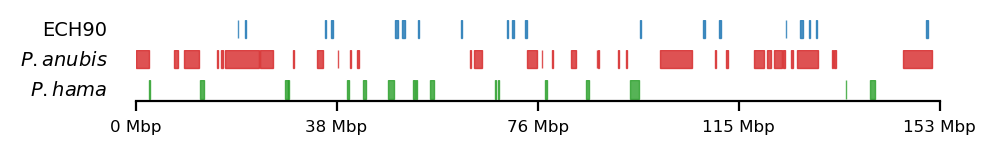
\includegraphics[width=5.1875in,height=0.80208in]{index_files/figure-latex/..-notebooks-07_various_plotting-fig-introduce-selected-regions-output-1.png}

}

\caption{\label{fig-introduce-selected-regions}Visual representation of
the selected regions for the baboon comparison. Shown are the ECH90
(top), high-olive (middle) and high-hama (bottom) regions, the basis of
the comparison of genomic intervals in this analysis. All coordinates
are lifted to the rheMac10 genome.}

\end{figure}%

\section{Chromatin Architecture}\label{chromatin-architecture}

The specific regions under strong selection identified across primate
species, including humans and baboons, are all located on the X
chromosome and span megabase-scale genomic regions. As mentioned above,
alternative mechanisms, such as the chromosomal architecture and its
rearrangements, could play critical roles in facilitating, regulating,
or buffering these regions from selective forces.

Therefore, understanding the genome organization and variation could
gain insights regarding mechanisms of selection as well. Chromatin has
long since been implicated in gene regulation and the functional state
of the cell (Lieberman-Aiden et al. 2009), as the three-dimensional
structure of the chromosome can bring distant regions in close
proximity, and disrupting the organization can lead to development
abnormalities (Dixon et al. 2015). Chromatin is hierarchically
compartmentalized, meaning multiple orders of organizaion can be nested
under each other. At the large end, compartments can span multiple
megabases (Lieberman-Aiden et al. 2009), and in the small end as little
as 500 base pairs have been showed to aid subgenic structural
organization. Even at sub-megabase scales, at the level of topologically
associating domains (TADs) or chromatin loops (Ramírez et al. 2018; Zuo
et al. 2021), the structure helps segregate regulatory elements and
ensure proper function.

Analyzing 3D chromatin data from rhesus macaques, a widely used primate
in experimental studies, could answer the question of whether regions
under selection are intertwined with chromosomal organizational
features. Studying the chromosomal architecture through gametogenesis,
particularly spermatogenesis, could provide valuable insights about
meiotic recombination and its relationship to genome organization. If
they correlate with regions under selection across primates, we have new
mystery to explain.

Wang et al. (2019) found that through the stages of spermatogenesis,
chromatin compartmentalization undergo massive reprogramming, going from
megabase-spanning compartments through smaller, \emph{refined}
compartments and back to the megabase compartments. The reprogramming is
conserved between rhesus macaque and mouse, indicating a very important
feature of the organization, but the author does not test whether
genomic positions of the compartments are conserved between species.
Extending their analysis of chromatin compartmentalization through
spermatogenesis could make an obvious starting point for investigating
the relationship between yet another set of megabase-spanning regions
and those of strong selection identified above.

\section{3C: Chromatin Conformation
Capture}\label{c-chromatin-conformation-capture}

The first method developed to capture long-range interactions between
pairs of loci was 3C, which uses spatially constrained ligation followed
by locus-specific PCR (Lieberman-Aiden et al. 2009). Subsequent
advancements introduced inverse PCR (4C) and multiplexed
ligation-mediated amplification (5C). A limitation common to these
methods is their inability to perform genome-wide, unbiased analyses, as
they require predefined pairs of target loci.

DNA can be organized into different structural levels. 3C focuses on
identifying the higher-order organization within the nucleus, such as
when the 30 nm chromatin fiber folds into loops, Topologically
Associating Domains (TADs), and chromatin compartments.

\section{Hi-C: High-Throughput 3C}\label{hi-c-high-throughput-3c}

The introduction of the Hi-C (high-throughput 3C) method
(Lieberman-Aiden et al. 2009) opened new possibilities for exploring the
three-dimensional organization of the genome, as deep-sequencing
technologies combined with high-performance computing allow for
genome-wide analysis that is unbiased. Lieberman-Aiden et al. (2009)
show that when combining spatially constrained ligation with deep
parallel sequencing and subsequent analysis, we can infer distinct
chromosomal territories as intrachromosomal contacts were significantly
less abundant than interchromosomal contacts. The method also confirmed
the spatial separation of two chromatin conformations in its active
(open) state or inactive (closed) state, as they were significantly
correlated with distances measured by fluorescence \emph{in-situ}
hybridisation (FISH). The two comformations were termed \emph{A}- and
\emph{B}-compartments, respectively, and A defined to positively
correlate with gene density. Finally, they showed that loci are
physically more proximal when they belong to the same compartment
implying that Hi-C reads serves well as a proxy for distance. Later,
several smaller-order domains were inferred with the same method, such
as topologically associating domains (TADs) and chromatin loops. Here,
we narrow our focus on the largest of the structures,
\emph{compartments}, that is known to determine availability to
transcription factors, thus making an \emph{A} compartment
\emph{active}---and the \emph{B} compartment \emph{inactive}.

\subsection{Hi-C Library preparation}\label{hi-c-library-preparation}

A specialized protocol for preparing the DNA library is necessary
(Lieberman-Aiden et al. 2009, fig. 1a). Briefly, formaldehyde is used to
crosslink spatially adjecent chromatin. Restriction enzyme
\emph{HindIII} is used to digest the crosslinked chromatin, leaving
sticky ends, \texttt{5-AGCT-3}, that are filled and biotinylated with a
polymerase (using either biotinylated A, G, C, or T). The strands are
ligated in highly dilute conditions, which is favoring the ligation of
the two crosslinked strands, forming chimeric, biotinylated strands.
Upon ligation, the restriction site is lost as a biotinylated
\texttt{5-CTAG-3} site (also referred to as the \emph{ligation
junction}) is formed. Lastly, the ligation junctions are isolated with
streptavidin beads and sequenced as a paired-end library.

To be able to create stage-resolved Hi-C library of spermatogenetis,
several steps have to be performed on the samples before crosslinking.
First, the samples have to be treated immediately after harvesting to
ensure viable cells. Secondly, the samples have to be purified to
accurately represent each stage og spermatogenesis. Specifically, the
data for this project (Wang et al. 2019, acc. GSE109344) preluded the
library preparation protocol by sedimentation-based cell sorting to
separate live spermatogenic cells into different stages of
differentiation, namely spermatogonia, pachytene spermatocyte, round
spermatid, and spermatozoa. Then, the cells were fixed in their
respective state before crosslinking. The authors use their own derived
method for library preparation, termed small-scale \emph{in-situ} Hi-C,
allegedly producing a high-quality Hi-C libary from as little as 500
cells (capturing the variance of millions of cells).

Initially, Hi-C library preparation was designed to generate molecules
with only a single ligation site in each, but with advancements in
sequencing technology (`short-reads' can now span several hundreds of
base pairs) and the shift to more frequently cutting restriction enzymes
for higher resolution results in multiple ligation events per sequenced
molecule (Open2C et al. 2024), which is adressed in the section below.

\subsection{Hi-C Data Analysis}\label{hi-c-data-analysis}

The analysis of the read-pairs of a Hi-C library is divided into several
smaller tasks, see Figure~\ref{fig-hic-analysis-flow}.

\begin{figure}

\centering{

\pandocbounded{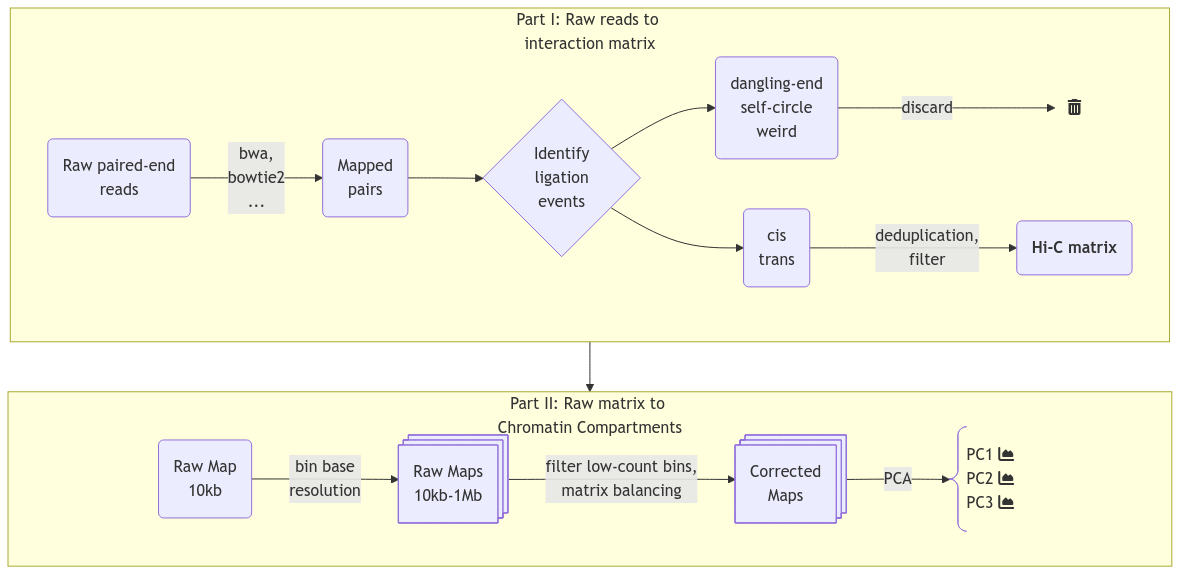
\includegraphics[keepaspectratio]{illustrations/fig-hic-data-analysis.png}}

}

\caption{\label{fig-hic-analysis-flow}A simplified pipeline for Hi-C
data analysis: from raw reads to a Hi-C interaction matrix. See
Table~\ref{tbl-ligation-events} for details on ligation events.}

\end{figure}%

We must align the reads to the reference in such a way that the
\emph{intentional} chimeric read-pairs (as per above-mentioned protocol)
are rescued, and \emph{unintentional} read-pairs are discarded. That is,
we must make sure they represent ligation junction of adjecent chromatin
segments, and not technical artefacts or unintentional (random) fusions
of unrelated DNA.

\subsubsection{Aligning the Hi-C reads}\label{aligning-the-hi-c-reads}

The main difference between Hi-C libraries and standard paired-end
libraries is the high fraction of chimeric reads in Hi-C. As a contact
pair is crosslinked and ligated before sequencing, chimeric reads occur
as a feature, and standard mapping techniques seeks to filter out this
type of reads (Lajoie, Dekker, and Kaplan 2015). Thus, we need
specialized tools for rescuing chimeric reads. That said, we have to be
cautious distinguishing the intended chimerism for Hi-C and that of
technical artefacts. Any software for local alignment can be used for
aligning reads from a Hi-C library. However, one should make sure to
disable paired-end rescue mode if possible, otherwise each read in a
pair (each mate) should be aligned separately (Lajoie, Dekker, and
Kaplan 2015). This removes the assumption that the distance between
mates fits a known distribution because the genomic sequences originate
from a continuous DNA-fragment. For example, the \emph{bwa-mem} (Li
2013) implementation of this (the \texttt{-P} option) activates the
Smith-Waterman algorithm to rescue missing hits, but disables the search
of hits that fit a `proper' pair. After alignment, each read is
typically assigned to the nearest restriction fragment to enable
categorization of pairs into different categories.

Interestingly, this last step is not included by default in
\emph{pairtools}, as Open2C et al. (2024) observe very similar
statistical properties on pairs that are either close or distant from
the nearest restriction site. Thus, restriction fragment filters are not
needed, and instead, a simple filter is applied against short-distance
pairs that is automatically calibrated.

\subsubsection{Identifying and Storing Valid Hi-C
Pairs}\label{identifying-and-storing-valid-hi-c-pairs}

One should be cautious when filtering invalid from valid pairs, as they
are not easily distinguished. A ligation event will be categorized into
one of five categories (see Table~\ref{tbl-ligation-events}):
\emph{dangling-end}, \emph{self-circle}, \emph{weird},
\emph{intrachromosomal} (cis), and \emph{interchromosomal} (trans)
(Bicciato and Ferrari 2022, Ch. 1). Either \emph{dangling-end} or
\emph{self-circle} events are reported if a read-pair maps to the same
restriction fragment depending on the orientation, and deemed
uninformative (Lajoie, Dekker, and Kaplan 2015). Usually, \emph{weird}
events are demeed uninformative as well, as it is challenging to
distinguish a sequencing error from the result of a diploid fragment.
PCR duplicates should be discarded as well, having either identical
genomic sequence, or sharing exact 5' alignment positions of the pair
(Lajoie, Dekker, and Kaplan 2015; Bicciato and Ferrari 2022, Ch. 1). The
probability that such pairs are valid (i.e.~there are multiple of the
same pairs) is very low. We also have to distinguish between molecules
with only a single ligation event (one-way contact) or multiple ligation
events (multi-way contacts). For that, a descision should be made on
whether to 1) discard molecules with multiple ligations, 2) report one
of the ligations (e.g.~the 5'-most in both directions), or 3) report all
events on a molecule.

\begin{longtable}[]{@{}
  >{\raggedright\arraybackslash}p{(\linewidth - 2\tabcolsep) * \real{0.2083}}
  >{\raggedright\arraybackslash}p{(\linewidth - 2\tabcolsep) * \real{0.7917}}@{}}
\caption{Five categories of ligation events and a short explanation.
\emph{Hi-C Data Analysis: Methods and Protocols Ch.
1}.}\label{tbl-ligation-events}\tabularnewline
\toprule\noalign{}
\begin{minipage}[b]{\linewidth}\raggedright
Event name
\end{minipage} & \begin{minipage}[b]{\linewidth}\raggedright
Explanation
\end{minipage} \\
\midrule\noalign{}
\endfirsthead
\toprule\noalign{}
\begin{minipage}[b]{\linewidth}\raggedright
Event name
\end{minipage} & \begin{minipage}[b]{\linewidth}\raggedright
Explanation
\end{minipage} \\
\midrule\noalign{}
\endhead
\bottomrule\noalign{}
\endlastfoot
Dangling-end & Non-digested collinear fragments. Fraction can be
high. \\
Self-circle & Collinear fragment(s) have circularized. Very low fraction
could indicate unsuccesful ligation. \\
Weird & Mates have the same orientation on the reference. Is not
possible with single copy fragment. Either sequencing errors or diploid
fragments\footnote{Bicciato and Ferrari (2022) mentions that this type
  of ligations had been used to model interaction between
  sister-chromatids post-replication in \emph{Drosophila}.}. \\
Cis & Pairs from the same chromosome (intrachromosomal) \\
Trans & Pairs from distinct chromosomes (interchromosomal) \\
\end{longtable}

\subsubsection{Quality Control and Interaction
Matrices}\label{sec-matrix-qc}

To determine the quality of the Hi-C library, most tools generate
quality control log files at some point during the filtering steps,
which can then be aggregated and analyzed (with e.g.~MultiQC Ewels et
al. (2016)). The ratios between the different ligation events can be
informative about the quality of the Hi-C library. Here, both the
distribution of discarded reads across categories, as well as the ratios
between \emph{cis}/\emph{trans} interactions for a certain organism
provide information about the library. For example, the biases of
different aligners might be captured by comparing the reason why reads
are discarded between two different aligners, as well as whether or not
there is a preference of \emph{cis} or \emph{trans} in an aligner
itself. This allows for evaluating the mapping parameters as well as the
filters applied downstream. Additionally, \(P(s)\), the contact
probability as a function of genomic separation can be inspected as it
should decay with increasing distance. The \emph{trans}/\emph{cis}-ratio
can sometimes be a good indicator of the noise level in the library, and
additionally, the level of random ligation events can be quantified by
counting the number of \emph{trans} events occurring to mitochondrial
genome. They should not occur naturally, as the mitochondrial genome is
separated from the DNA in the nucleus. This method has some pitfalls
that should be controlled for; some parts of the mitochondrial genome
can be integrated into the host genome, and mitochondrial count may
differ between cell-stages.

Typically, a filter against low mapping quality is applied on the data
before constructing the interaction matrix (Hi-C matrix), and a
conventional threshold is \(mapq < 30\) (Bicciato and Ferrari 2022).
However, a considerable amount of reads do not pass that threshold, and
thus we risk discarding potential valid information and should make sure
to have enough data. Consequently, \emph{HicExplorer} defaults to a
lower threshold (\(mapq < 15\)), and \emph{pairtools} enforces no filter
by default, but recommends setting this manually (starting at
\(mapq < 30\)).

A Hi-C interaction matrix simply maps the frequency of interactions
between genomic positions in a sample. The maximum resolution of a Hi-C
matrix is defined by the restriction enzyme, where the size of the
restriction site (probabilistically) determines average space between
each cut. With a 4 bp restriction site, the fragments will average
\(4^4 = 256 bp\) and similarly \(4^6 = 4096 bp\) for a 6 bp restriction
site. This leads to \textasciitilde12,000,000 and \textasciitilde800,000
fragments, respectively. Very deep sequencing is required to achieve
enough coverage to analyze the interaction matrix at the restriction
fragment resolution, but, usually, such high resolution is not required.
Therefore, it is common practice to bin the genome into fixed bin sizes,
which also enables a more efficient handling of the data if the full
resolution is not needed (e.g.~when plotting large regions such as a
whole chromosome). The conventional format to store a Hi-C matrix,
consisting of large multidimensional arrays, is HDF5. Each HDF5 file can
store all resolutions and metadata about the sample, resolutions
typically ranging from 10kb to 1Mb. Typically, the stored resolutions
should be multiples of the chosen base-resolution, as the lower
resolutions are constructed by recursive binning of the base resolution.
\emph{cooler} (Abdennur and Mirny 2020) neatly offers efficient storage
with sparse, upper-triangle symmetric matrices and naming-conventions of
the groups in their \emph{.h5}-based file format, \emph{.cool}, and they
provide a Python class \texttt{Cooler} as well for efficiently fetching
and manipulating the matrices in Python.

\subsubsection{Inferring from the matrix (Calling
Compartments)}\label{inferring-from-the-matrix-calling-compartments}

The raw frequency matrices are generally not very informative, as the
contact frequencies vary greatly between bins and contain biases in
addition to the \(P(s)\) decay, which results in a diagonal-heavy matrix
with high amount of noise the further we travel from the diagonal.
Therefore, to analyze the three-dimensional structure of the chromatin,
a method for correcting (or balancing) the raw Hi-C matrix has to be
applied. It is unadvisable to correct low-count bins as it will greatly
increase the noise, or to correct very noisy bins, or very high-count
bins. Therefore, some bin-level filters are applied before balancing
(Lajoie, Dekker, and Kaplan 2015);

\begin{itemize}
\tightlist
\item
  Low-count bins are detected by comparing bin sums to the distribution
  of bin sums with a percentile cutoff,
\item
  Noisy bins are detected by comparing bin variance to the variance
  distribution of all bins (and percentile cutoff), and
\item
  Outlier point-interactions are removed (a top-percentile of bin-bin
  interactions)
\end{itemize}

A widely used balancing method is Iterative Correction and
Eigendecomposition (ICE) (Imakaev et al. 2012), which utilizes a
data-driven approach for correcting multiplicative biases. Briefly, ICE
is based on an assumption of equal visibility of all loci, and uses the
pairwise and genome-wide structure to generate a set of biases along
with a map of relative interaction frequencies by iteratively dividing
each row, then each column, by its mean until convergence. This results
in a uniform coverage profile (corrected coverage), yielding a smoother
interaction matrix with slower transitions, thus greatly reducing
visibility-induced biases. It does not distinguish between the sources
of biases, and thus calculates a collective bias for each position.
Imakaev et al. (2012) show that \emph{known} biases are factorizable by
comparing their results to predictions of restriction fragment biases,
GC content, and mappability from a computationally intensive
probabilistic approach. By showing that the product of those known
biases explain \(>99.99%
\) of the variability in their bias estimation, they argue that both
known and unknown biases will be captured with their iterative
correction method (also denoted \emph{matrix balancing}).

Even with a binned, filtered, and balanced matrix, we are still left
with the challenge of translating the matrix into biologically relevant
inferations. Importantly, we have to remember that the matrix arise from
a collection of cells and that the interaction frequency cannot be
translated to a fraction of cells. Additionally, the effect from
averaging interaction patterns can cause both individual patterns to be
burried and the average pattern to show a pattern that does not exist in
any of the single cells. Therefore, when pooling matrices one must make
sure that the samples are as similar as possible (e.g.~the same
differentiation stage and so on). We can also not distinguish
interactions that either co-occur in the same cell or ones that are
mutually exclusive. Lastly, the way interaction patterns are defined
poses a challenge; we define the chromatin compartments to be the output
of a method, the `E' in `ICE', eigendecomposition, not as a specific
pattern that we can explicitly search for. Although experimentally
verified to tightly correlate with chromatin states (Lieberman-Aiden et
al. 2009), the inferred compartments vary with different methods of
calculating the eigenvector, as dicussed in
Section~\ref{sec-methods-eigendecomposition} and
Section~\ref{sec-results-eigenvectors}. To further complicate the
challenge, interaction patterns on different scales co-exist and are
difficult to disentangle without simplifying assumptions such as
small-scale interactions are not visible (or they are negligible) at a
certain resolution, or restricting the viewframe to eliminate
large-scale variance between chromosome arms. It is by definition a
speculative exercise to interpret the biological relevance of an
observed pattern, but the consensus is to call compartments on
interacting regions that arise from the eigendecomposition of a Hi-C
matrix without further modifications (Lajoie, Dekker, and Kaplan 2015).
As the eigenvector is only unique up to a sign change, a phasing track
is used to orient the eigenvector, aiming for a positive correlation
with GC content (in mammals), making A-compartments represent the active
euchromatin, and B-compartments the closed heterochromatin.

\subsubsection{Compartment Edges and Genomic
Intervals}\label{compartment-edges-and-genomic-intervals}

As arbitrarily as a compartment may be defined, we chose to define
another genomic interval for analysis. It is well known that CTCF and
other structural proteins preferentially binds to Topologically
Associating Domains (Bicciato and Ferrari 2022, Ch. 3) (TADs; they were
initially defined as sub-Mb chromatin structures (Lajoie, Dekker, and
Kaplan 2015), but currently the definition seems to vary based on the
method of extraction (Open2C et al. 2022)). Derived from this, we define
a transition zone between A/B compartments to look for enrichment of
specific regions of interest.

We can test if two sets of genomic intervals correlate (say, compartment
edges and ECH regions) by either proximity of the non-intersecting parts
of the sets, or by intersection over union (Jaccard index). When the
underlying distribution of a statistic (or index) is unknown, a
widespread method in statistics for estimating a p-value is by
bootstrapping. Here, one of the sets are bootstrapped (the intervals are
placed at random positions) a number of times, \(b\), and the fraction
of statistics more extreme than the one we observe is reported as the
p-value.

\section{Reproducibility
Infrastructure}\label{reproducibility-infrastructure}

\begin{codelisting}

\caption{\label{lst-reproduce}Three simple steps to re-create the
project.}

\centering{

\begin{Shaded}
\begin{Highlighting}[numbers=left,,]
\FunctionTok{git}\NormalTok{ clone https://github.com/munch{-}group/hic{-}spermatogenesis.git}
\ExtensionTok{conda}\NormalTok{ env create }\AttributeTok{{-}f}\NormalTok{ binder/environment.yml}
\ExtensionTok{gwf}\NormalTok{ run}
\end{Highlighting}
\end{Shaded}

}

\end{codelisting}%

Reproducibility is a cornerstone of the scientific method, ensuring that
findings can be independently verified and built upon by others. Without
it, the credibility of research findings is undermined, hindering
scientific progress by becoming anecdotal. The necessity of
reproducibility also aligns with scientific skepticism---the practice of
critically evaluating evidence and methods to guard against biases or
errors. As research grows increasingly computational, robust
reproducibility infrastructure is essential to maintain these principles
(Baker 2016), facilitating transparency, validation, and collaboration
across diverse scientific disciplines. Thus, apart from the biological
questions we seek to investigate and answer in this thesis, a major goal
is to create fully (and easily) reproducible results through a
self-contained and version-controlled pipeline using git (Torvalds and
Hamano 2005), GitHub (GitHub, Inc. n.d.), quarto (Allaire et al. 2024),
Anaconda (Anaconda Software Distribution 2016), gwf (GenomeDK 2023), and
Jupyter (Kluyver et al. 2016). The result is a fully reproducible
analysis, including figures and tables in only 3 lines of
code\footnote{And access to a high-performance computer with at least 12
  TB storage and 32 CPU-cores, and a couple of days waiting time (else
  \texttt{gwf\ run} will fail as it asks for a lot of resources).}
(Listing~\ref{lst-reproduce}) . See Table~\ref{tbl-reproducibility} for
a brief overview:

\begin{longtable}[]{@{}
  >{\raggedleft\arraybackslash}p{(\linewidth - 2\tabcolsep) * \real{0.1944}}
  >{\raggedright\arraybackslash}p{(\linewidth - 2\tabcolsep) * \real{0.8056}}@{}}
\caption{Overview of the tools used for reproducibility of this
thesis.}\label{tbl-reproducibility}\tabularnewline
\toprule\noalign{}
\begin{minipage}[b]{\linewidth}\raggedleft
Tool
\end{minipage} & \begin{minipage}[b]{\linewidth}\raggedright
Description
\end{minipage} \\
\midrule\noalign{}
\endfirsthead
\toprule\noalign{}
\begin{minipage}[b]{\linewidth}\raggedleft
Tool
\end{minipage} & \begin{minipage}[b]{\linewidth}\raggedright
Description
\end{minipage} \\
\midrule\noalign{}
\endhead
\bottomrule\noalign{}
\endlastfoot
Jupyter & Interactive coding environment for analysis and development
(notebooks are natively rendered with Quarto) \\
Quarto & A Quarto Manuscript project nested inside a Quarto Book for
rendering html (website) and PDF (manuscript) from Markdown via Pandoc.
Supports direct embedding of output from Jupyter Notebook cells (plots,
tables). \\
Conda & For managing software requirements and dependency versions
reproducibly. \\
git & Version control and \texttt{gh-pages} branch for automated render
of Quarto project \\
GitHub & Action was triggered \texttt{on\ push} to render the project
and host on
\href{https://munch-group.org/hic-spermatogenesis/}{munch-group.org} \\
\emph{gwf} & Workflow manager to automate the analysis on a HPC cluster,
wrapped in Python code. \texttt{workflow.py} currently does everything
from \texttt{.fastq} to \texttt{.cool}, but notebooks can be set to run
sequentially as part of the workflow as well. \\
\end{longtable}

\subsection{GWF: workflow management for High-Performance Computing
(HPC)}\label{gwf-workflow-management-for-high-performance-computing-hpc}

To enable consistently reproducing the analyses, a workflow manager is
utilized. Several exist, but the most well-known is likely Snakemake.
However, we use the pragmatic (authors' own words), lightweight workflow
manager GWF, which is optimized for the GenomeDK insfrastructure, and
has the benefit of in-house support.

Briefly, GWF works on a python script, conventionally
\texttt{workflow.py}, that wraps all the jobs (\emph{targets} in gwf
lingo) you will submit to the HPC cluster. Each target is submitted from
a template, written as a Python function, which includes \texttt{inputs}
and \texttt{outputs} that GWF should look for when building the depency
graph, \texttt{options} list of resources that is forwarded to the
queueing system (Slurm in our case), and \texttt{specs}, specifying the
submission code in Bash as a formatted Python string (meaning we can
pass Python variables to the submission code), providing an extremely
flexible framework for running large and intensive analyses in a
high-performance computing environment.

\subsection{Project Initialization}\label{project-initialization}

\subsubsection{\texorpdfstring{\emph{gwf}}{gwf}}\label{gwf}

The initialization of the project directory is the basis of
reproducibility and transparency, together with \texttt{workflow.py}
inhabiting the main directory. Specifically, it includes a subdirectory
for (intermediate) files that are produced by the pipeline,
\texttt{steps/}. Everything in this directory is reproducible simply by
re-running the \emph{gwf}-workflow. It is thus not tracked by
\texttt{git}, as the large files (raw reads, aligned read-pairs, etc.)
it contains are already indirectly tracked (\texttt{workflow.py} is
tracked). It can be safely deleted if your system administrator tells
you to free up disk space, although you would have to run the workflow
again to continue the analysis. Several directories are created for
files that are not produced by the pipeline, that is, files that the
workflow uses, configuration files, figures edited by hand, etc.
Ideally, as few files as possible should be outside of \texttt{steps/},
to be as close as possible to an automated analysis.

\subsubsection{Jupyter Notebooks}\label{jupyter-notebooks}

A \texttt{notebooks/} subdirectory contains Jupyter notebooks that are
named chronologically, meaning they operate on data located in either
\texttt{steps/} or generated from a previous notebook. This way, the
workflow can also be set up to run the notebooks (in order) to produce
the figures, tables, and their captions used in this manuscript.

\subsubsection{Quarto}\label{quarto}

Quarto is an open-source scientific and technical publishing system that
uses (pandoc) markdown to create and share production quality output,
integrating Jupyter Notebooks with Markdown and LaTeX and enabling
embedding content across \emph{.ipynb} and \emph{.qmd}. In \emph{.qmd},
code chunks in several programming languages can be executed and
rendered, including Python, R, mermaid (JavaScript-based diagramming). A
Quarto project is configured with a YAML configuration file
(\texttt{\_quarto.yml}) that defines how output is rendered. In this
project, we use a nested structure, nesting a \emph{Slides} project and
a \emph{Manuscript} project inside a \emph{Book} project. To manage the
directory as a Quarto Book project, a quarto configuration file was
placed at the base, defining how the Book should be rendered.
Additionally, configuration files were placed in \texttt{slides/} and
\texttt{thesis/}, to render them as Quarto Slides and Quarto Manuscript,
respectively. This nested structure lets us render different subprojects
with different configurations than the main project, for example to
generate the manuscript, a single Quarto Markdown file, in both
\emph{.html} and \emph{.pdf}, and only including embedded outputs from
specified cells from notebooks in the parent directory. Although the
Quarto framework is extensive, it is still under development and has
several drawbacks worth mentioning. First, one can only embed the output
of code cells from notebooks, meaning the only way to embed text with a
python variable (e.g.~you want the manuscript to reflect the actual
value of a variable, sample sizes
\texttt{n\ =\ {[}1000,\ 10000,\ 100000{]}}, and their respective
outputs) is by converting a formatted python string into Markdown and
send it to the output. Second, embedded figures will be copied as-is in
the notebook, and thus cannot be post-processed with size or layout.
This makes it impractical to e.g.~use the same figures in slides and in
the manuscript. Third, when rendering large projects that is tracked by
git, some output files (that have to be tracked to publish the website)
can exeed GitHub size limits. Especially if rendering in the \emph{jats}
format, producing a MECA Bundle that should be the most flexible way to
exchange manuscripts. However, as not applicable to this thesis, the
option was simply disabled. Fourth, some functionality relies on
external dependencies that cannot be installed on a (linux) remote host
(GenomeDK), such as relying on a browser for converting \texttt{mermaid}
diagrams into png for the pdf-manuscript.

\subsection{git and GitHub}\label{git-and-github}

To track the project with git and GitHub, the abovementioned structure
was initialized as a GitHub repository, including a workflow for GitHub
Actions to publish and deploy the website on the \texttt{gh-pages}
branch when pushing commits to \texttt{main}. Briefly, it sets up a
virtual machine with Quarto and its dependencies, renders the project as
specified in the \texttt{\_quarto.yml} configuration file(s), and
publishes the project on the group website
\href{https://munch-group.org/hic-spermatogenesis}{munch-group.org}.

\chapter{Methods}\label{methods}

All computations were performed on GenomeDK (GDK), an HPC cluster
located on Aarhus Uninversity, and most of the processing of the data
was made into a custom GWF workflow, a workflow manager developed at
GDK.

With the analysis tools determined in the above section, I decided it
was not feasible to follow the exact approach as Wang et al. (2019) with
any of HiCExplorer and Open2C, as they use a third software, HiC-Pro.
For mapping the raw reads, Hic-Pro internally uses bowtie2 in end-to-end
mode, followed by trimming the 3'-end of the unmapped reads, then
remapping the 5'-ends to rescue chimeric fragments. I initially mapped
the reads using end-to-end Bowtie2 without the rescue-remapping feature,
resulting in a very high fraction of discarded reads. Manually
implementing the remapping approach would be impractical. When
reanalyzing data, it is important to use state-of-the-art tools.
Considering the release timeline (e.g., HiC-Pro v3.1.0 in 2021), both
HiCExplorer and Open2C are more recent and likely offer better support
for current methodologies. Additionally, the HiC-Pro pipeline stops at a
normalized contact map, and is thus not sufficient for downstream
analysis. In hindsight, it would have been more sensical to use HiC-Pro
to get normalized contact maps, then continue analyzing with
cooler/cooltools, and finally compare the results evenly with the
results achieved from using Open2C from start to finish.
Figure~\ref{fig-hic-tools-comparison} gives an overview of the 3
pipelines metioned in this report.

\begin{figure}

\centering{


\includegraphics[width=0.8\linewidth,height=0.5\textheight]{illustrations/placeholder2000x360.png}

}

\caption{\label{fig-hic-tools-comparison}A 3-column flow of HiC-Pro,
HiCExplorer, and Open2C}

\end{figure}%

\section{Fetching raw data}\label{fetching-raw-data}

To reproduce the results from Wang et al. (2019), I chose to use their
raw data directly from the SRA portal {[}ref{]}. I filtered the data to
contain all their paired-end Hi-C reads, and included only macaque
samples. The dataset also contains RNAseq data, and the same tissues for
both macaque and mouse. The metadata for the dataset was extracted into
a runtable \texttt{SRA-runtable.tsv}. To get an overview of the data
accessions used in this analysis, we will first summarize the runtable
that contains the accession numbers and some metadata for each sample
(Table~\ref{tbl-runtable-summary}). It adds up to \textasciitilde1Tb of
compressed \texttt{fastq} files, holding \textasciitilde9.5 billion
reads, roughly evenly spread on the 5 tissue types.

\begin{longtable}[]{@{}lllll@{}}

\caption{\label{tbl-runtable-summary}Summary of the data accessions used
in this analysis}

\tabularnewline

\toprule\noalign{}
& source\_name & GB & Bases & Reads \\
\midrule\noalign{}
\endhead
\bottomrule\noalign{}
\endlastfoot
0 & fibroblast & 211.403275 & 553,968,406,500 & 1,846,561,355 \\
1 & pachytene spermatocyte & 274.835160 & 715,656,614,700 &
2,385,522,049 \\
2 & round spermatid & 243.128044 & 655,938,457,200 & 2,186,461,524 \\
3 & sperm & 164.131640 & 428,913,635,400 & 1,429,712,118 \\
4 & spermatogonia & 192.794420 & 518,665,980,300 & 1,728,886,601 \\

\end{longtable}

\subsection{Fetching and indexing the
reference}\label{fetching-and-indexing-the-reference}

Wang et al. (2019) use the 2006-version of the macaque reference,
\emph{rheMac2}. Supporting my previous sentiment about not using
outdated resources I find it most reasonable to use the latest
reference, \emph{rheMac10}, where Warren et al. (2020) have improved
contiguity from \emph{rhemac8} by 120 fold, going from N50 contig size
of 107 Kbp to 46 Mbp. Reproducing the analysis on the latest assembly of
the macaque genome should therefore gain a more accurate read mapping,
and consequently a better inference of the chromatin compartments.
Therefore, \emph{rheMac10} was downloaded to GDK from UCSC web servers.
To use bwa for mapping, \emph{rheMac10} needs to be indexed with both
bwa-index with the \texttt{-\/-bwtsw} option and samtools-faidx, which
results in six indexing files for bwa-mem to use. Both bwa-mem and
bowtie2 were used in different configurations, and bowtie2 requires its
own indexing of the reference, using bowtie2-build with the
\texttt{-\/-large-index} option, which creates six index files for
\texttt{bowtie2} to use. The options \texttt{-\/-bwtsw} and
\texttt{-\/-large-index} create the special indexing format required for
large genomes such as macaque. As we use the position of the centromere
to partition chrX into its two arms, and no comment about it was made by
Warren et al. (2020), the centromeric region was inferred (visually)
from the UCSC browser view of \emph{rheMac10}, where a large continuous
region (chrX:57.5Mb-60.2Mb) had no annotation and showed many repeating
regions. The region is roughly the same region as inferred by Wang et
al. (2019) by the same method.

\section{HiCExplorer trials}\label{hicexplorer-trials}

To get aligned reads in a format compatible with HiCExplorer, the read
mates have to be mapped individually to the reference genome. This
supports the old convention to avoid the common heuristics of local
aligners used for regular paired-end sequencing libraries (Lajoie,
Dekker, and Kaplan (2015)). HiCExplorer provide examples for both
\emph{bwa} and \emph{bowtie2}, so I used both with recommended settings.
In both cases, the aligner outputs a .bam-file for each mate
(\texttt{sample\_R1.bam} and \texttt{sample\_R2.bam}), and HiCExplorer
performs the parsing, deduplication, and filtering of the reads and
builds the raw interaction matrix in a single command,

\begin{Shaded}
\begin{Highlighting}[]
\ExtensionTok{hicBuildMatrix} \AttributeTok{{-}s}\NormalTok{ sample\_R1.bam sample\_R2.bam }\AttributeTok{{-}o}\NormalTok{ matrix.h5 }\PreprocessorTok{[}\SpecialStringTok{...}\PreprocessorTok{]}
\end{Highlighting}
\end{Shaded}

For parsing, the command needs a \texttt{-\/-restrictionCutFile},
locating the restriction sites from the restriction enzyme used on the
reference genome, which is generated with \texttt{hicFindRestSites} that
operates on the reference genome and restriction sequence. The default
filter, \texttt{-\/-minMappingQuality\ 15}, was applied as described in
Section~\ref{sec-matrix-qc}. Notably, HiCExplorer has no options on
handling multiple ligations, and the method is undocumented. I assume
that Ramírez et al. (2018) have implemented a conservative handling
(masking all multiple ligations), as that would have the least
consequence.

\begin{figure}

\centering{


\includegraphics[width=0.7\linewidth,height=\textheight,keepaspectratio]{illustrations/placeholder2000x360.png}

}

\caption{\label{fig-hicexplorer-workflow}Overview of the target
templates used for hicexplorer. As most operations are handled by
\texttt{hicBuildMatrix}, it is rather simple.}

\end{figure}%

\begin{longtable}[]{@{}lllll@{}}

\caption{\label{tbl-hic-exploration}The samples chosen for initial data
exploration with HiCExplorer. From NCBI SRA Portal.}

\tabularnewline

\toprule\noalign{}
& Run & Bases & Bytes & source\_name \\
\midrule\noalign{}
\endhead
\bottomrule\noalign{}
\endlastfoot
0 & SRR6502335 & 73201141800 & 31966430779 & fibroblast \\
1 & SRR6502336 & 65119970100 & 24433383054 & fibroblast \\
2 & SRR6502337 & 52769196300 & 23015357755 & fibroblast \\
3 & SRR6502338 & 52378949100 & 22999581685 & fibroblast \\
4 & SRR6502339 & 28885941600 & 10960123150 & fibroblast \\

\end{longtable}

For the initial exploration of methods with HiCExplorer, I chose five
fibroblast samples (see Table~\ref{tbl-hic-exploration}). The goal was
to replicate some of the figures from Wang et al. (2019) using
HiCExplorer, especially to reconstruct interaction matrices and E1
graphs from macaque data. We constructed matrices with
\texttt{hicBuildMatrix} as described from the separately mapped
read-pairs. Along with the matrix \emph{.h5} file, a \emph{.log} file
was created as well, documenting the quality control for the sample.
Multiple logs were aggregated and visualized with \texttt{hicQC}.

Before correction (or balancing) of the interaction matrix, a
pre-correction filter is applied, filtering out low-count bins and very
high-count bins. A threshold for Mean Absolute Deviation (MAD) is
estimated by \texttt{hicCorrect\ diagnostic\_plot}, followed by
iterative correction with
\texttt{hicCorrect\ correct\ -\/-correctionMethod\ ICE}. The PCA was
performed with \texttt{hicPCA} on the corrected matrices, yielding the
first 3 PCs.

The matrix plotting function, \texttt{hicPlotMatrix}, plots matrices
directly to .png, and so there is no output sent to the Jupyter display.
As I kept the analysis in a Jupyter Notebook (using the buikt-in
shell-escape commands to execute \texttt{bash} code), the plot files
must be embedded back into the notebook. The command-line options for
modifying plots are quite limited, such as adding spacing for a bigWig
track with E1 values, including plot titles, or defining the size and
resolution of the plot. I made a brief attempt to implement a custom
plotting function for the .h5 matrices and bigWig tracks. However, this
approach had a major limitation: it could not fetch specific regions
from the matrix dynamically and instead required loading entire matrices
into memory, including full-length chromosomes.

\section{Open2C pipeline}\label{open2c-pipeline}

\begin{figure}

\centering{

\pandocbounded{
\includegraphics[keepaspectratio]{illustrations/placeholder2000x360.png}}

}

\caption{\label{fig-flowchart-handling-coolers}Showing the GWF target
templates used with the Open2C pipeline. As it is highly modular, it is
also a bit elaborate.}

\end{figure}%

A GWF workflow was created to handle the first part of the data
processing, and each accesion number (read pair, mate pair) from the
Hi-C sequencing was processed in parallel, so their execution was
independent from each other.

\subsubsection{Downloading the reads}\label{downloading-the-reads}

The reads were downloaded from NCBI SRA with SRA-toolkit (DevTeam 2024)
directly to GDK using the docker image \emph{wwydmanski/sra-downloader}
as gunzipped \texttt{.fastq} files. Although possible to provide a list
of accessions to the toolkit, I submitted each accession as a separate
target, as SRA-Toolkit acts sequentially, and only starts the next
download after all compression tasks were done. It was therefore a
low-hanging fruit to parallelize the download for efficiency.

\subsubsection{Mapping Hi-C reads}\label{mapping-hi-c-reads}

Suspiciously, ({``{Open2C}''} n.d.) do not mention any problems with
aligning the Hi-C reads, they just provide an example using bwa-mem in
paired-end mode and with the \texttt{-P} option set, which activates the
Smith-Waterman (Li 2013) algorithm to rescue missing hits, by focusing
on assigning only one of the mates to a good mapping and escape
mate-rescue. The documentation of
\href{https://bio-bwa.sourceforge.net}{\texttt{bwa}} state that both
bwa-mem and bwa-sw will rescue chimeric reads. Consequently, Open2C does
not have a buikt-in way of pairing the reads after mapping, and the
reads were thus mapped using Open2C's recommendations, using their
established pipeline for producing a cooler. I chose the latter, where I
mapped the fastq files to \emph{rheMac10} in paired end mode for a pair
(\(m1\), \(m2\)) with \texttt{bwa\ mem\ -SP\ rheMac10\ m1\ m2}.

\subsubsection{Parse and sort the reads}\label{parse-and-sort-the-reads}

We need to convert the alignments into ligation events, and distinguish
between several types of ligation events. The simplest event is when
each side only maps to one unique segment in the genome `UU'. Other
events, where one or both sides map to multiple segments or the reads
are long enough (\(>150bp\)) to contain two alignments (multiple
ligations) have to be considered as well. Multiple ligations are called
\emph{walks} by Open2C, and are treated according to the
\texttt{-\/-walks-policy} when parsing the alignments into valid pairs
(or valid Hi-C contacts). Here, \texttt{mask} is the most conservative
and masks all complex walks, whereas \texttt{5unique} and
\texttt{3unique} reports the 5'-most or 3'-most unique alignment on each
side, respectively, and \texttt{all} reports all the alignments. The
pairs are piped directly into \texttt{pairtools\ sort} after parsing, as
the deduplication step requires a sorted set of pairs. The
\emph{.pairs}-format produced by \texttt{pairtools} is an extension the
\href{https://data.4dnucleome.org/file-formats/pairs/}{4DN
Consortium}-specified format, storing Hi-C pairs as in
Table~\ref{tbl-pairsformat}.

\begin{longtable}[]{@{}
  >{\raggedleft\arraybackslash}p{(\linewidth - 4\tabcolsep) * \real{0.1644}}
  >{\raggedright\arraybackslash}p{(\linewidth - 4\tabcolsep) * \real{0.1644}}
  >{\raggedright\arraybackslash}p{(\linewidth - 4\tabcolsep) * \real{0.6712}}@{}}
\caption{Column specification of the .pairs format as extended by
pairtools.}\label{tbl-pairsformat}\tabularnewline
\toprule\noalign{}
\begin{minipage}[b]{\linewidth}\raggedleft
Index
\end{minipage} & \begin{minipage}[b]{\linewidth}\raggedright
Name
\end{minipage} & \begin{minipage}[b]{\linewidth}\raggedright
Description
\end{minipage} \\
\midrule\noalign{}
\endfirsthead
\toprule\noalign{}
\begin{minipage}[b]{\linewidth}\raggedleft
Index
\end{minipage} & \begin{minipage}[b]{\linewidth}\raggedright
Name
\end{minipage} & \begin{minipage}[b]{\linewidth}\raggedright
Description
\end{minipage} \\
\midrule\noalign{}
\endhead
\bottomrule\noalign{}
\endlastfoot
1 & read\_id & the ID of the read as defined in fastq files \\
2 & chrom1 & the chromosome of the alignment on side 1 \\
3 & pos1 & the 1-based genomic position of the outer-most (5') mapped bp
on side 1 \\
4 & chrom2 & the chromosome of the alignment on side 2 \\
5 & pos2 & the 1-based genomic position of the outer-most (5') mapped bp
on side 2 \\
6 & strand1 & the strand of the alignment on side 1 \\
7 & strand2 & the strand of the alignment on side 2 \\
8 & pair\_type & the type of a Hi-C pair \\
9 & mapq1 & mapq of the first mate \\
10 & mapq2 & mapq of the second mate \\
\end{longtable}

I initially used \texttt{-\/-walks-policy\ mask}, and later followed the
recommendations from \emph{pairtools}, specifically informing that
longer reads (\(>150bp\)) might have a significant proportion of reads
that contain complex walks. With this in mind and as the average
read-length of our data is 300 bp, I decided to re-parse the alignments
into a new set of pairs, and equally apply the recommended filter (next
section). As both results are saved, we can compare the two approaches.

\subsubsection{Filter and deduplicate
pairs}\label{filter-and-deduplicate-pairs}

Pairtools comes with a de-duplication function, \texttt{dedup}, to
detect PCR duplication artefacts. At this point I removed all reads that
mapped to an unplaced scaffold. Even though \emph{rhemac10} is less
fragmented than \emph{rhemac8} , \emph{rheMac10} still contains more
than 2,500 unplaced scaffolds, which are all uninformative when
calculating the chromatin compartments as is the goal of this analysis.
Therefore, we simply only include the list of conventional chromosomes
(1..22, X, Y) when doing the deduplication. Initially, the default
values were used to remove duplicates, where pairs with both sides
mapped within 3 base pairs from each other are considered duplicates.
\texttt{cooler} recommend to store the most comprehensive and unfiltered
list of pairs, and then applying a filter it on the fly by piping from
\texttt{pairtools\ select}. The first run that was parsed with
\texttt{mask} was not filtered for mapping quality. After reparsing the
alignments and applying the same analysis, we compare the two pipelines.
A quality control report is generated by \texttt{pairtools\ dedup} as
well, and the reports are merged and visualized with \texttt{MultiQC}
(Ewels et al. 2016) for each cell type.

\subsubsection{Create interaction matrices
(coolers)}\label{create-interaction-matrices-coolers}

The final part of the GWF workflow takes \texttt{.pairs} as input and
outputs a \texttt{.cool} file (a \emph{cooler}). Initially, I read
directly from the newly generated deduplicated pairs without additional
filtering, but the official recommendation is to filter out everything
below \(mapq = 30\) by piping the pairs through
\texttt{pairtools\ select\ "(mapq1\textgreater{}=30)\ and\ (mapq2\textgreater{}=30)"}
to \texttt{cooler\ cload\ pairs}. I re-parsed the alignments and created
new coolers, including only the Hi-C contacts where \(mapq \leq 30\),
following the current recommendations from Open2C.

\subsubsection{Pooling samples (Merging
coolers)}\label{pooling-samples-merging-coolers}

The samples are grouped into \emph{replicates} with a unique BioSample
ID, and I chose to pool all the interaction matrices for each cell type.
Even though it is slightly unclear how their replicates are defined,
Wang et al. (2019) determine compartments to be highly reproducible
between replicates, and they are pooling the replicates as well.

\texttt{cooler\ merge} was used to merge all samples in each cell-type
directory to just one interaction matrix for each cell type. The
function merges matrices of the same dimensions by simply adding the
interaction frequencies of each genomic position together, resulting in
less empty or low-count bins.

\subsubsection{Create multi-resolution coolers
(zoomify)}\label{create-multi-resolution-coolers-zoomify}

A feature of working inside the ecosystem of Open2C is that it natively
provides support for storing sparse interaction matrices in multiple
resolutions in the same file by adding HDF5-groups to the
(multires-)cooler. We can then efficiently store resolutions (i.e.,
different bin sizes) that is multiples of the smallest bin size. We
chose to use 10kb, 50kb, 100kb, and 500kb bins, and the resolutions are
made by recursively binning the base resolution. Abdennur and Mirny
(2020) call this process zoomifying, and \texttt{cooler\ zoomify} does
the job (it recursively calls \texttt{cooler\ coarsen} to merge bins).

\subsubsection{Matrix balancing (Iterative
correction)}\label{matrix-balancing-iterative-correction}

Finally, we balance (or correct) the matrices using the cooler CLI. We
use \texttt{cooler\ balance} with the default options which iteratively
balances the matrix (Iterative Correction).

We balance the matrices on each resolution, and thus it cannot be done
prior to zoomifying. Abdennur and Mirny (2020) state that the balancing
weights are resolution-specific and will no longer retain its biological
meaning when binned with other weights. Therefore, we apply
\texttt{cooler\ balance} to each resolution separately.
\texttt{cooler\ balance} will create a new column in the \texttt{bins}
group of each cooler, \texttt{weight}, which can then be included or not
in the downstream analysis. This means we will have access to both the
balanced and the unbalanced matrix.

The default mode uses genome-wide data to calculate the weights for each
bin. It would maybe be more suitable to calculate the weights for
\emph{cis} contacts only, and that is possible through the
\texttt{-\/-cis-only} flag, and that can be added to another column, so
that we can compare the difference between the two methods easily.
However, when adding the option, the process seemed to stall and had to
be terminated manually, and it was not investigated further.

\subsubsection{Eigendecomposition}\label{sec-methods-eigendecomposition}

The eigendecomposition of a Hi-C interaction matrix is performed in
multiple steps. As value of the eigenvector is only \emph{significant}
up to a sign, it is convention to use GC content as a phasing track to
orient the vector. E1 is defined to be positively correlated with GC
content, meaning a positive E1 value signifies an active chromatin
state, which we denote a A-type compartment (or simply A-compartment).
We performed eigendecomposition of two resolutions, 100 kbp and 500 kbp.
Wang et al. (2019) briefly describes their method to calculate the
eigenvectors as a sliding window approach on the observed/expected
matrix in 100 kb resolution summing over 400 kb bins with 100 kb step
size, a method I was not able to replicate in the \emph{Open2C}
ecosystem. I decided to mimic this by smoothing the 100 kb E1 values by
summing to 500 kb bins in steps of 100 kb, yielding a comparable
resolution which I denote `\emph{pseudo}-500 kb' resolution
(\emph{ps500kb}).

First, we calculate the GC content of each bin of the reference genome,
\emph{rheMac10}, which is binned to the resolution of the Hi-C matrix we
are handling. It is done with \texttt{bioframe.frac\_gc}
(\emph{Open2C}). To calculate the E1 compartments, we use only
within-chromosome contacts (\emph{cis}), as we are not interested in the
genome-wide contacts. \texttt{cooltools.eigs\_cis} will decorrelate the
contact-frequency by distance before performing the eigendecomposition.
\texttt{eigs\_cis} needs a \emph{viewframe} (view) to calculate E1
values, the simplest view being the full chromosome. However, when there
is more variance between chromosome arms than within arms, the sign of
the first eigenvector will be determined largely by the chromosome arm
it sits on, and not by the chromatin compartments. To mitigate this, we
apply a chromosome-arm-partitioned view of the chromosome.

Additionally, to mimic the \emph{Local PCA} from (Wang et al. 2019), I
also defined a view of 10 Mb bins. Thoughout the project, I will compare
results from each of the three views and resolutions, and they will be
referred to as `full', `arms', and `10Mb' views.

\subsubsection{Plotting matrices}\label{plotting-matrices}

We use matplotlib (Team 2024) and seaborn (Waskom 2021) to plot in the
Open2C framework. Utilizing the \texttt{Cooler} class, we can fetch
regions of the matrix without modifying the file. As my analysis is
centered around the X chromosome, it is efficiently handled by simply
fetching `chrX' from the matrix with
\texttt{cooler.Cooler.matrix().fetch(\textquotesingle{}chrX\textquotesingle{})}.
Many methods of the cooler class returns data selectors, which do not
retrieve data before it is queried (Abdennur and Mirny 2020). This means
we can create many selectors at once without overflowing memory,
enabling us to plot multiple interaction matrices side-by-side, e.g.~the
corrected and un-corrected matrices. This is easily done with the
\texttt{balance} parameter of the matrix selector (\texttt{.matrix()}),
which determines if it should apply the balancing weights to the
coordinates and defaults to \texttt{True}.

The matrix is retrieved and plotted with
\texttt{matplotlib.pyplot.matshow}, which automatically produces a
heatmap image of the matrix. Here, instead of transforming the
interaction matrix, the color scale is log-transformed with
\texttt{matplotlib.colors.LogNorm}. Additionally, \texttt{cooltools}
comes with more tools to aid visualization: \emph{adative coarsegrain}
and \emph{interpolation}, which can be chained.
\texttt{adaptive\_coarsegrain} iteratively coarsens an array to the
nearest power of two and refines it back to the original resolution,
replacing low-count pixels with NaN-aware averages to ensure no zeros in
the output, unless there are very large regions that exceed the
\texttt{max\_levels} threshold, such as the peri-centromeric region.

I implemented a plotting utility, \texttt{plot\_for\_quarto} in notebook
\texttt{07\_various\_plotting.ipynb} that is compatible with the YAML
cell-options read by Quarto's \texttt{embed} shortcode. It will take an
arbitrary number of samples and plot a chromosome (or region) with or
without its respective E1 value for either of the three viewframes which
has been created. The input is a (subsetted) \emph{pandas DataFrame},
defined from a file search matching a pattern specified to the
\texttt{glob} Python module.

\section{Genomic Intervals}\label{genomic-intervals}

\subsection{Full Regions, Edges, and
Limits}\label{full-regions-edges-and-limits}

From the eigenvectors, the A-compartments were extracted in
bedgraph-format
(\texttt{{[}\textquotesingle{}chrom\textquotesingle{},\ \textquotesingle{}start\textquotesingle{},\ \textquotesingle{}end\textquotesingle{}{]}})
and compared with ECH90 regions lifted to \emph{rheMac10} from human. We
perform visual inspection of the genomic intervals and test whether
ECH90 regions are enriched near the edges of the compartments by
defining a 200 kilobase transition-zone centered at each sign change of
E1 (referred to as \emph{compartment edge}). We compare genomic
intervals (or sets) both visually by plotting the regions, and by a
proximity test and bootstrapping the Jaccard index. Additionally, the
compartment limits were invetigated (only 1 flanking base pair) in the
same manner. Additionally, the limits were extracted from the baboon
datasets and lifted to \emph{rheMac10} for comparison.

\subsubsection{Proximity test}\label{proximity-test}

Determines whether the non-overlapping segments of the sets are more
proximal than expected by chance. We define the \emph{annotation} set
and the \emph{query} set, and the distance from each interval on the
\emph{query} to the most proximal interval on the \emph{annotation} is
used to generate an index of proximity by the mean distance to nearest
interval in the \emph{annotation}. Then, bootstrapping (\(b = 100000\))
is performed by randomly placing the query intervals to generate the
null distribution, and finally, the fraction of the \emph{null} as
extreme or more extreme as our observed proximity is reported as the
p-value.

\subsubsection{Jaccard test}\label{jaccard-test}

Measures the significance of the observed Jaccard index (intersection
over union) between two sets. The index is a measure of
\emph{similarity} (\(intersection/union\)) between two sets (between 0
and 1), which is very sensitive to the size difference between the sets,
as even when comparing a set of intervals to a small subset of itself
will yield a very small Jaccard index. When we use bootstrapping to
generate a null distribution (shuffling the intervals of the
\emph{query}), we find the probability that the two sets (with their
respective number and size of intervals), are as similar or more than
what we observe. The ratio is reported as the p-value. However, this
approach is still sensitive to flipping of query/annotation (if the
regions are not the same size), as only the query is bootstrapped.

\subsubsection{Multiple testing}\label{multiple-testing}

Considerations were made to avoid multiple testing biases (p-hacking):
Performing tests on all combinations of variables (cell type,
resolution, viewframe, query) will yield 90 p-values for each test, and
we would have to adjust the significance threshold (with
\(\alpha = 0.05\), we expect 4 tests passing the threshold by chance).
However, I will narrow down the parameter space based on visualizations
and reasoning, leaving fewer combinations to test. I do not find it
necessary to correct the conventional significance threshold,
\(\alpha=0.05\).

\chapter{Results}\label{results}

\section{HicExplorer Trials}\label{hicexplorer-trials-1}

\subsection{Quality Control}\label{quality-control}

The separately mapped read-mates were parsed into a \emph{.h5}
interaction matrix by \texttt{hicBuildMatrix}, which include a
\emph{.log} file documenting the buikt-in quality control (hereafter,
\emph{QC}). Log files from the 5 samples were merged with \texttt{hicQC}
(Figure~\ref{fig-explorer-all-3-qc}). I observe equal fractions of the
read-orientation of read-pairs (Figure~\ref{fig-explorer-all-3-qc},
left, row 5), which is expected for a good Hi-C library. Additionally,
it determines between 40\% to 50\% of the total reads to be valid Hi-C
contacts (Figure~\ref{fig-explorer-all-3-qc}, left, row 1), which is
usually only 25\%-40\% (as described in HiCExplorer docs).
Figure~\ref{fig-explorer-all-3-qc} (left, row 4) shows, however,
unusually high fractions of \emph{inter}-chromosomal contacts (up to
30\%) compared to \emph{intra}-chromosomal contacts (also denoted
\emph{trans} and \emph{cis} contacts, respectively). It is expected that
\emph{cis} contacts are orders of magnitude more frequent than
\emph{trans} contacts (Bicciato and Ferrari 2022, 2301:236;
Lieberman-Aiden et al. 2009), and HiCExplorer states it is usually below
10\% for a high-quality library. The high fraction may be mitigated by
enforcing a stricter \emph{mapq} threshold for a valid Hi-C pair, as we
also observe higher-than expected valid contacts. However, we continue
with the current matrices.

To compare how well these mappings perform, the plotting QC results is
an easy way. Therefore, the reads were mapped with \emph{bowtie2} in
both end-to-end- and local-mode followed by \texttt{hiCBuildMatrix}, and
the QC from each method was plotted next to each other
(Figure~\ref{fig-explorer-all-3-qc}). Interestingly, \emph{bowtie2} was
much more computer-intensive in both modes, perhaps because of the
\texttt{-\/-very-sensitive} option. In any case, the QC reveals a major
difference in the total number of reads that are determined to be valid
Hi-C contacts by \texttt{hicBuildMatrix}. As expected, mapping with
\emph{end-to-end-bowtie2} makes locating Hi-C contacts more difficult
than the other methods (Figure~\ref{fig-explorer-all-3-qc}, row 1),
finding a very low amount of mappable, unique pairs passing the quality
threshold. In contrast, mapping with \emph{local-bowtie2} performs
similarly to \emph{bwa} in finding mappable, unique, high-quality pairs,
but calls only approximately half the number of valid Hi-C contacts
(\textgreater20\%), resulting in a fraction of valid Hi-C pairs that
hits the expectation from \emph{HicExplorer} docs (row3). With
\emph{bwa}, the reads were discarded either due to low mapping quality
or non-unique mates, whereas with \emph{local-bowtie2}, the reads were
almost exclusively filtered out due to low mapping quality. This must be
a result of how the mappers assign mapping quality, and I believe
\emph{local-bowtie2} looks suspiciously selective in finding unique but
low quality alignments. \emph{end-to-end-bowtie} almost exclusively
filters out read-pairs where one mate is unmapped, which is expected
when the majority of reads are unmapped.

\begin{figure}[H]

\centering{

\pandocbounded{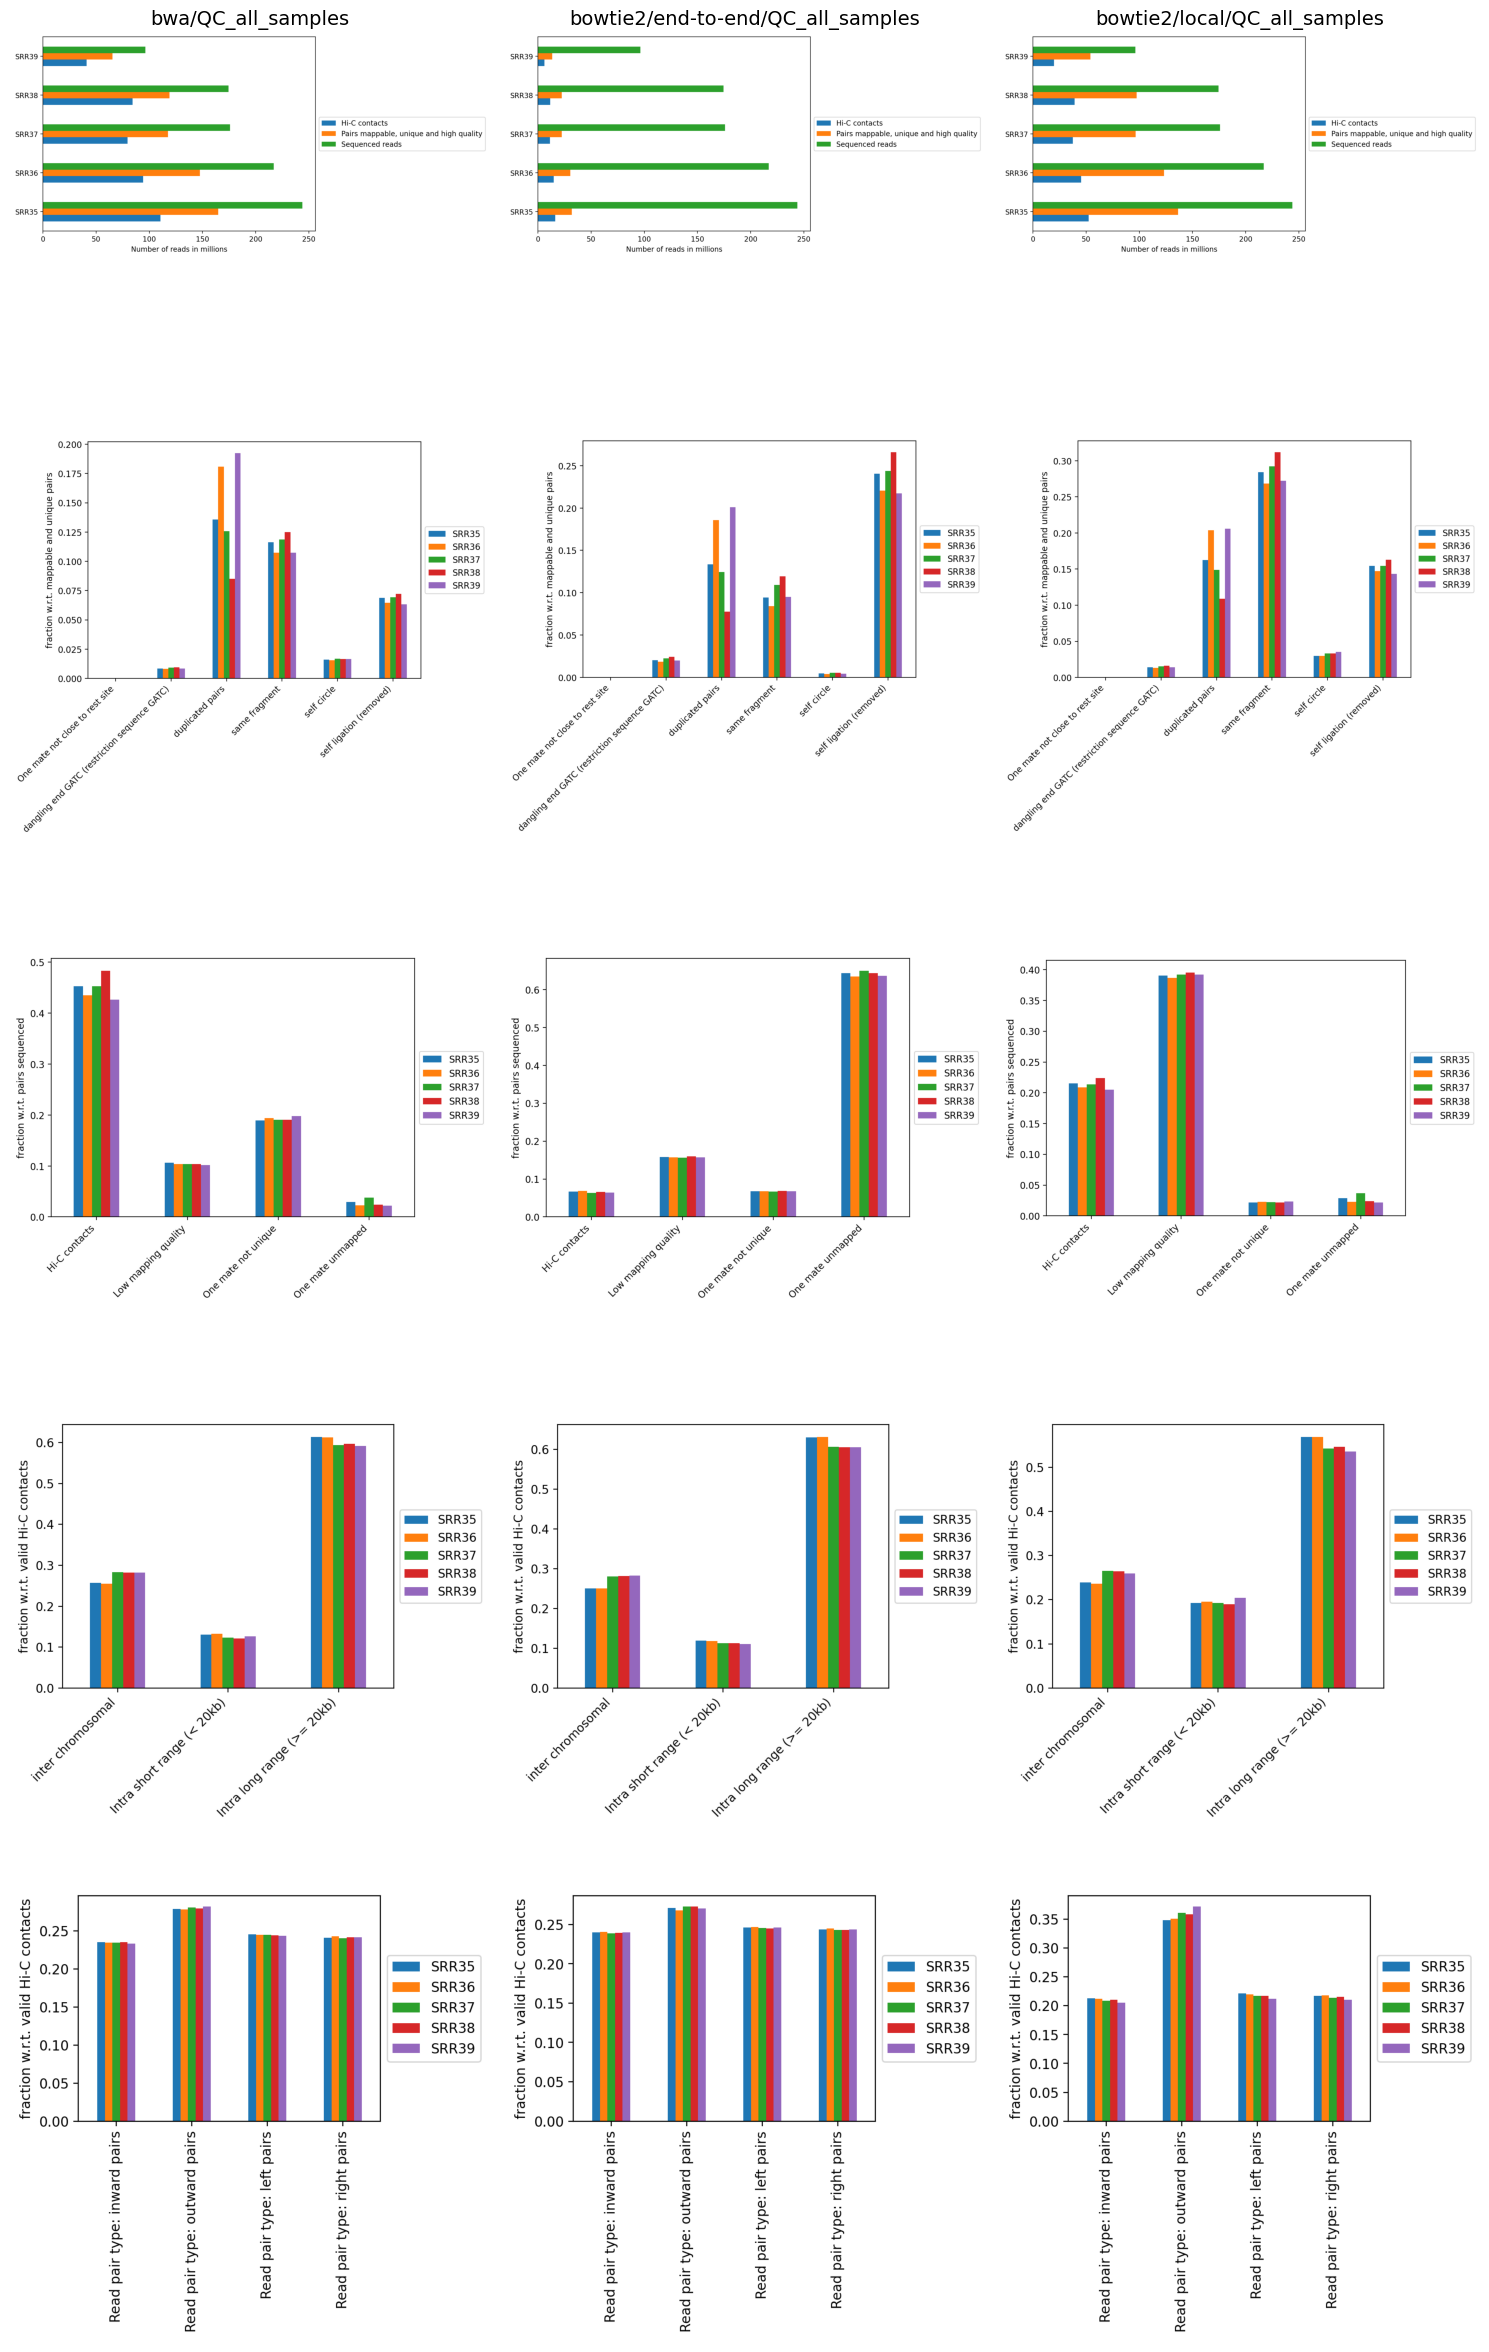
\includegraphics[keepaspectratio]{index_files/figure-latex/..-notebooks-01_hicexplorer-fig-explorer-all-3-qc-output-1.png}}

}

\caption{\label{fig-explorer-all-3-qc}Comparison of HiCExplorer QC plots
for all samples using different alignment tools. The rows represent
different QC plots (pairs sequenced, pairs discarded,
unmappable/non-unique, distance, and read orientation), and the columns
represent the 3 alignments used (BWA, Bowtie2 end-to-end, Bowtie2
local). Generated by \texttt{hicQC}.}

\end{figure}%

\subsection{Correction}\label{correction}

The correction diagnostic tool yielded a similar \emph{mad} threshold
within the range \([-3,-2]\). Even so, I followed the \emph{HicExplorer}
recommendation to set the lower threshold to at least -2 and the upper
threshold to 5 in the pre-normalization filter. I argue that with a high
number of valid contacts, it is safer to err on the side of caution and
maybe filter out bad data.

\begin{figure}

\begin{minipage}{0.06\linewidth}
~\end{minipage}%
%
\begin{minipage}{0.29\linewidth}

\centering{

\pandocbounded{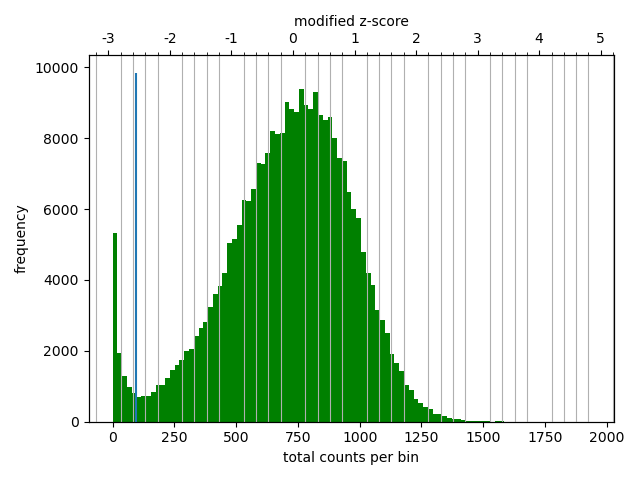
\includegraphics[keepaspectratio]{../figures/bwa/SRR6502335_diag_plot.png}}

}

\subcaption{\label{fig-explorer-pre-correction-SRR6502335}SRR6502335}

\end{minipage}%
%
\begin{minipage}{0.29\linewidth}

\centering{

\pandocbounded{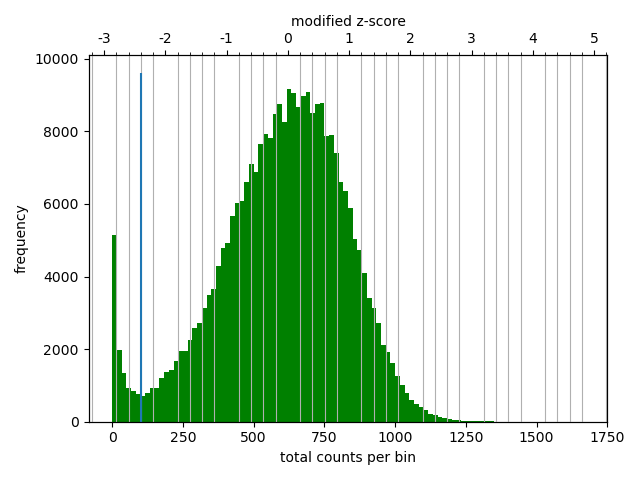
\includegraphics[keepaspectratio]{../figures/bwa/SRR6502336_diag_plot.png}}

}

\subcaption{\label{fig-explorer-pre-correction-SRR6502336}SRR6502336}

\end{minipage}%
%
\begin{minipage}{0.29\linewidth}

\centering{

\pandocbounded{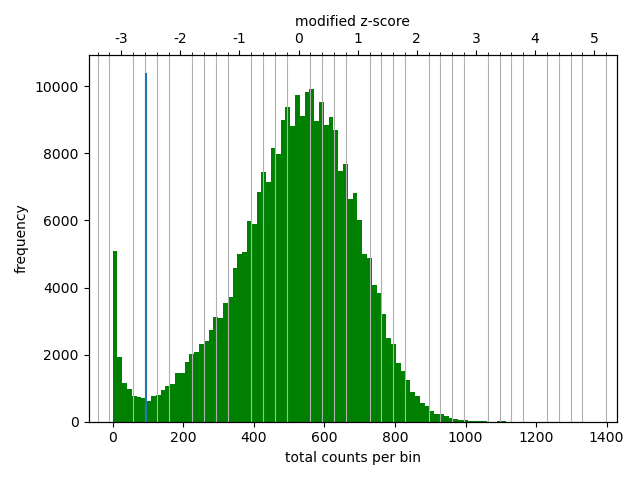
\includegraphics[keepaspectratio]{../figures/bwa/SRR6502337_diag_plot.png}}

}

\subcaption{\label{fig-explorer-pre-correction-SRR6502337}SRR6502337}

\end{minipage}%
%
\begin{minipage}{0.06\linewidth}
~\end{minipage}%
\newline
\begin{minipage}{0.21\linewidth}
~\end{minipage}%
%
\begin{minipage}{0.29\linewidth}

\centering{

\pandocbounded{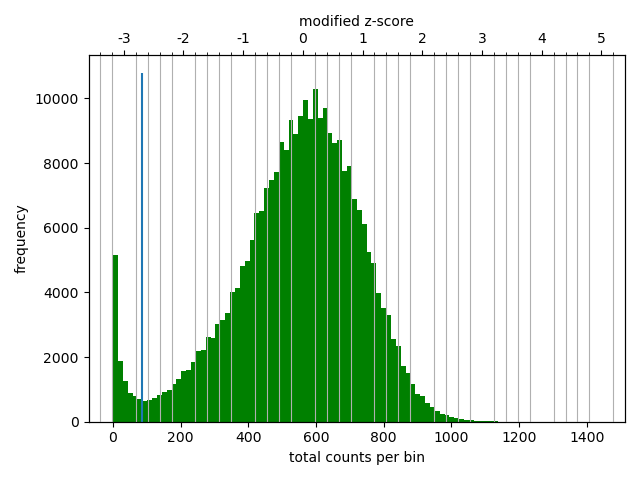
\includegraphics[keepaspectratio]{../figures/bwa/SRR6502338_diag_plot.png}}

}

\subcaption{\label{fig-explorer-pre-correction-SRR6502338}SRR6502338}

\end{minipage}%
%
\begin{minipage}{0.29\linewidth}

\centering{

\pandocbounded{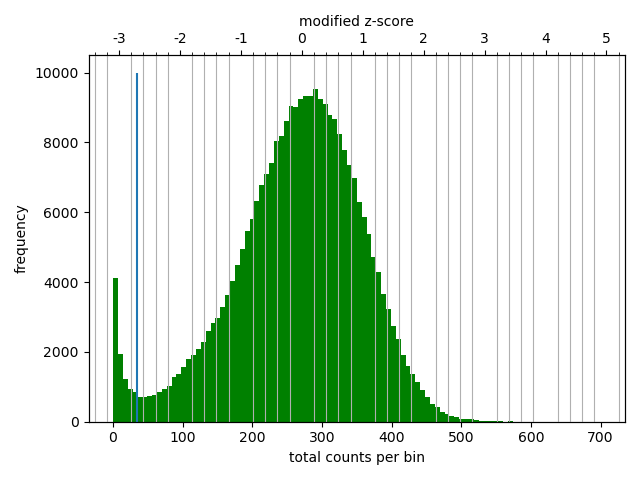
\includegraphics[keepaspectratio]{../figures/bwa/SRR6502339_diag_plot.png}}

}

\subcaption{\label{fig-explorer-pre-correction-SRR6502339}SRR6502339}

\end{minipage}%
%
\begin{minipage}{0.21\linewidth}
~\end{minipage}%

\caption{\label{fig-explorer-pre-correction}Histograms of the number of
counts per bin (bottom x-axis) and the modified z-score (top x-axis)
from which the \emph{mad} threshold is defined.}

\end{figure}%

As discussed, the five samples were pooled with \texttt{hicSumMatrices},
and the non-standard contigs (unplaced scaffolds) were filtered out, and
the different resolutions were created (\texttt{hicMergeMatrixBins}).
\emph{HiCExplorer} also comes with a normalization function prior to
correcting the matrix, which should be applied if different samples
should have comparable bin counts. It has no effect when having only one
matrix. Nevertheless, the pooled matrix was normalized and then
corrected compared in Figure~\ref{fig-explorer-pooled-norm-normcorr}. It
is now obvious why we have to correct the matrix. The uncorrected
(Figure~\ref{fig-explorer-pooled-chrX-norm}) has no signal apart from
the diagonal. Even though some bins have been filtered out, the expected
\emph{plaid} pattern of a contact matrix is visible along the diagonal
after the correction (Figure~\ref{fig-explorer-pooled-chrX-normcorr}),
leaving evidence for chromatin structure, especially in the first 50
million bases of the chromosome. There is a wide region of empty values
at the place of the centromere.

\begin{figure}

\begin{minipage}{0.50\linewidth}

\centering{

\pandocbounded{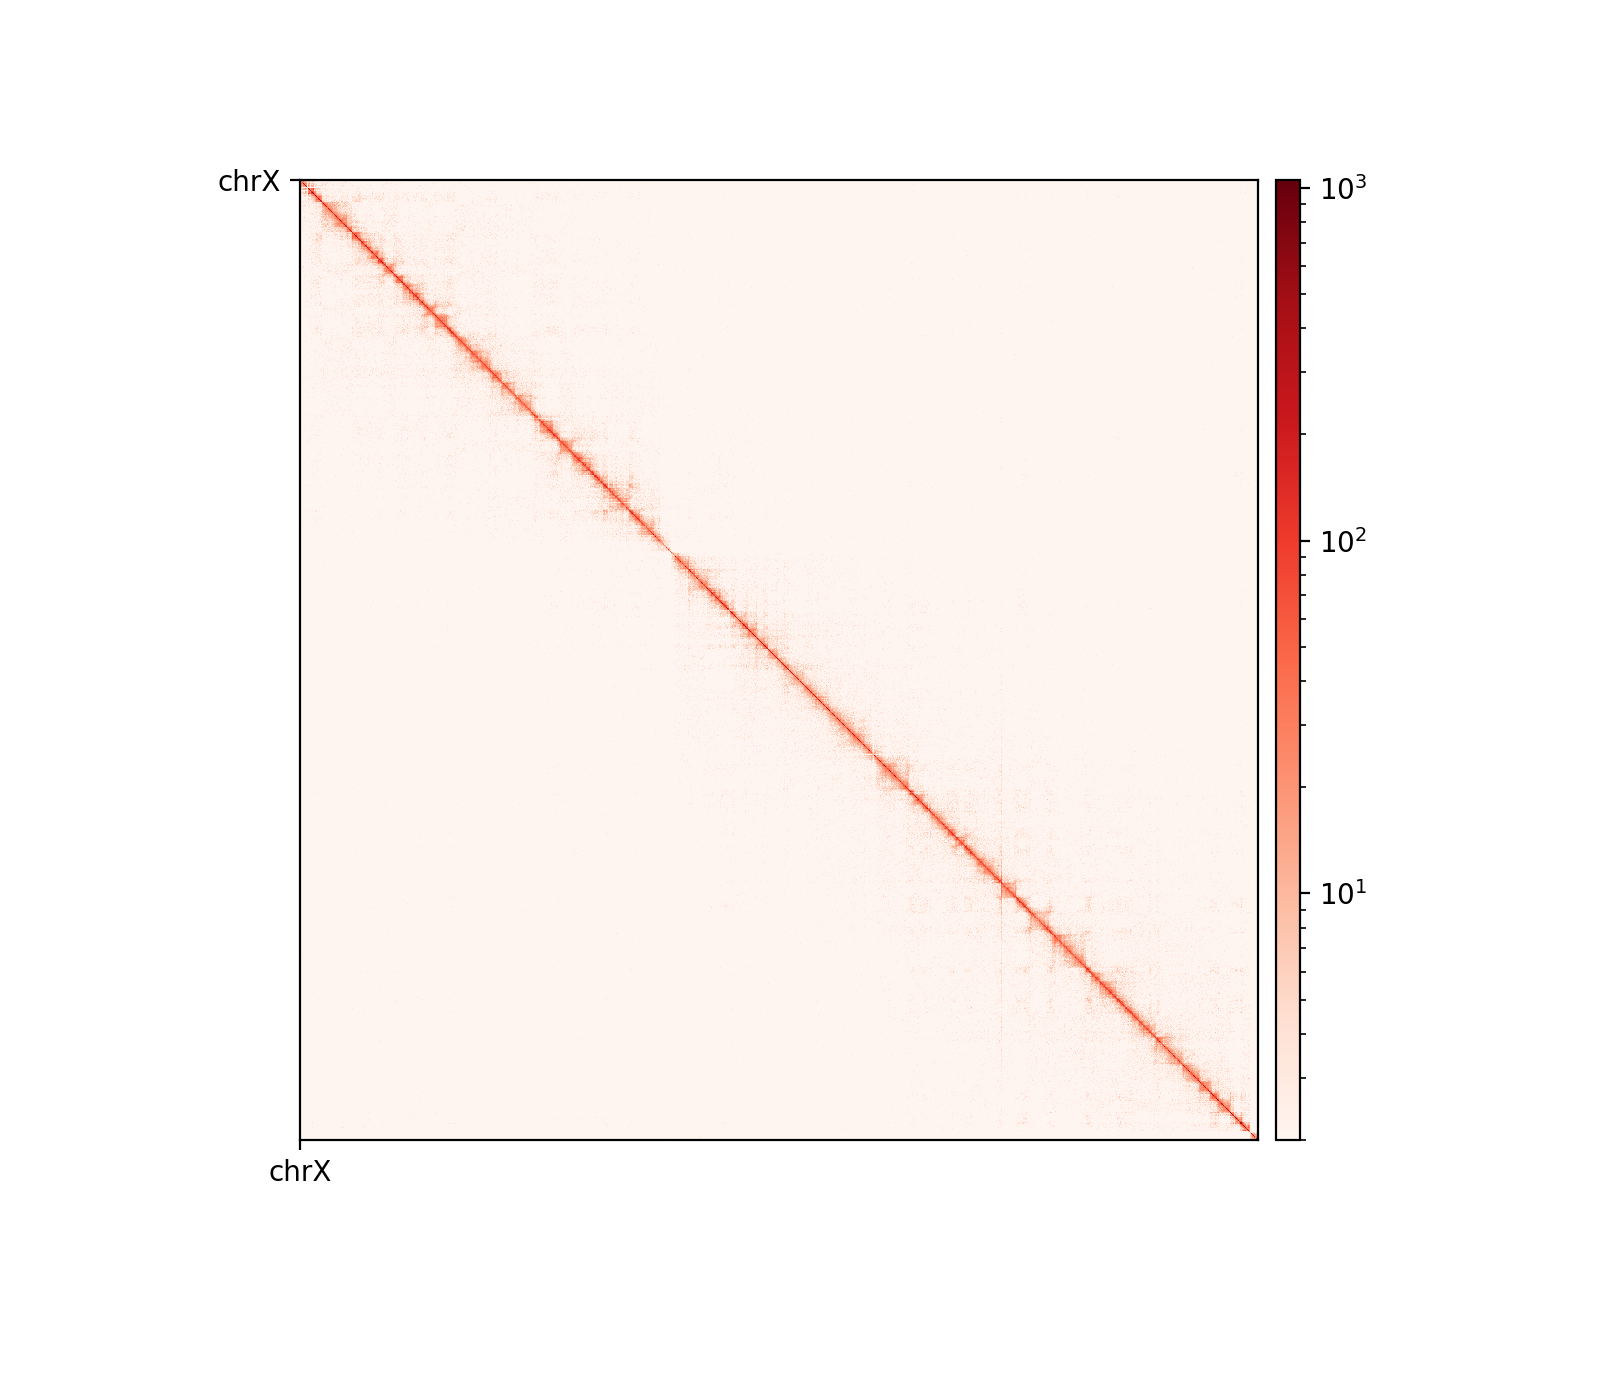
\includegraphics[keepaspectratio]{../figures/bowtie2/local/filter_pooled_50kb_chrX.png}}

}

\subcaption{\label{fig-explorer-pooled-chrX-norm}Normalized matrix chrX}

\end{minipage}%
%
\begin{minipage}{0.50\linewidth}

\centering{

\pandocbounded{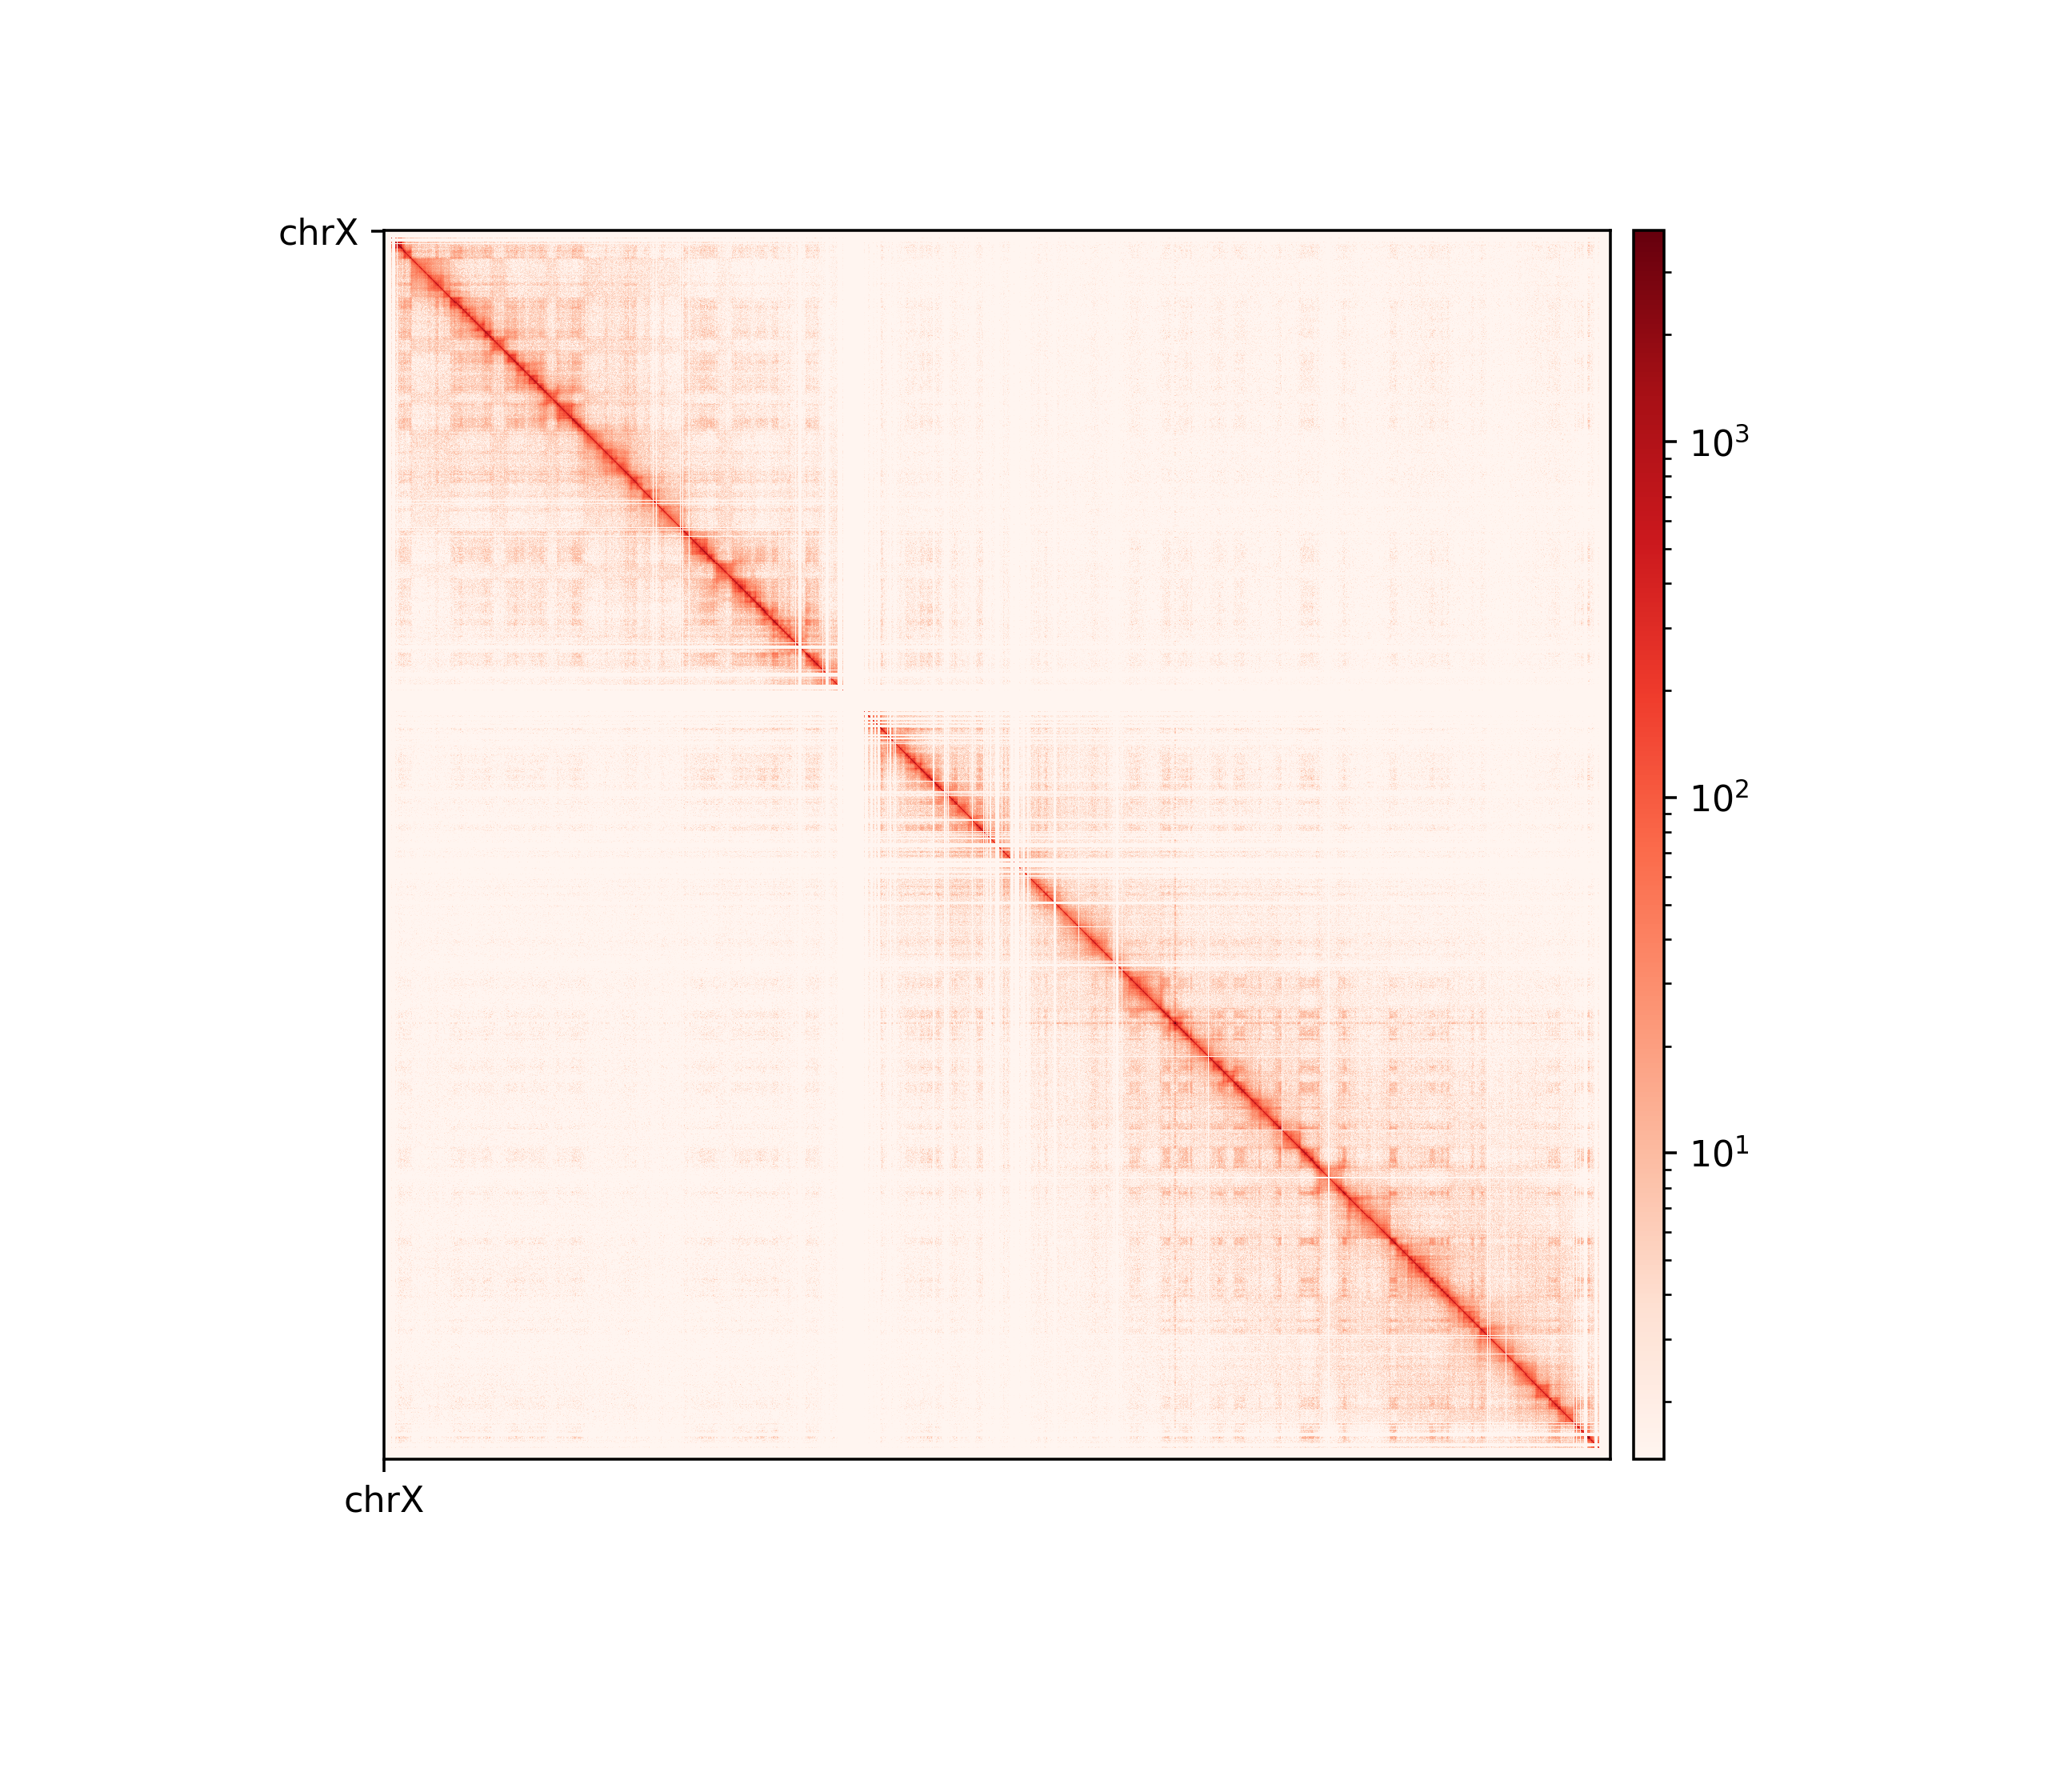
\includegraphics[keepaspectratio]{../figures/bowtie2/local/normalized/normsm_filter_pooled_100kb_corrected_chrX-full.png}}

}

\subcaption{\label{fig-explorer-pooled-chrX-normcorr}Normalized and
corrected chrX}

\end{minipage}%

\caption{\label{fig-explorer-pooled-norm-normcorr}A comparison of
interaction matrices before/after iterative correction
(\emph{HiCExplorer}).}

\end{figure}%

\subsection{Eigenvectors}\label{eigenvectors}

The PCA performed by \texttt{hicPCA} on the pooled samples at both 50kb
and 100kb resolution yielded the first 3 principal components. For PC1
on both resolutions (Figure~\ref{fig-explorer-pc1-50kb},
Figure~\ref{fig-explorer-pc1-100kb}) we observe only a single sign
change which occurs at around 60 Mbp, the region of the centromere. It
means the PCA has captured more variance between the chromosome arms
than within them, making it uninformative about chromatin compartments.
Upon visual inspection, it is clear that neither of the PC graphs
capture the pattern of the interaction matrix by its change of sign. It
seems the PCs capture variance from a bias that varies slowly and
predictably along the chromosome. The first PC that is supposed to
capture the compartments very suspiciously changes sign at the region of
the centromere, a classic problem that could be solved by restricting
the values from which the PC is calculated along the chromosome.
Unimpressed, I rationalize that the option \texttt{-\/-extra-track} to
provide a gene track or histone coverage should not affect this result
much. It should be provided as a phasing track to orient the eigenvector
to positively correlate with gene density or histone marks, and could
possibly muddle the compartments if not included. I followed
\emph{HiCExplorer} pipeline to plot and explore the matrices. At this
point, I stoppped using \emph{HiCExplorer}, as I assessed that a more
flexible tool was needed.

\begin{figure}

\begin{minipage}{0.33\linewidth}

\centering{

\pandocbounded{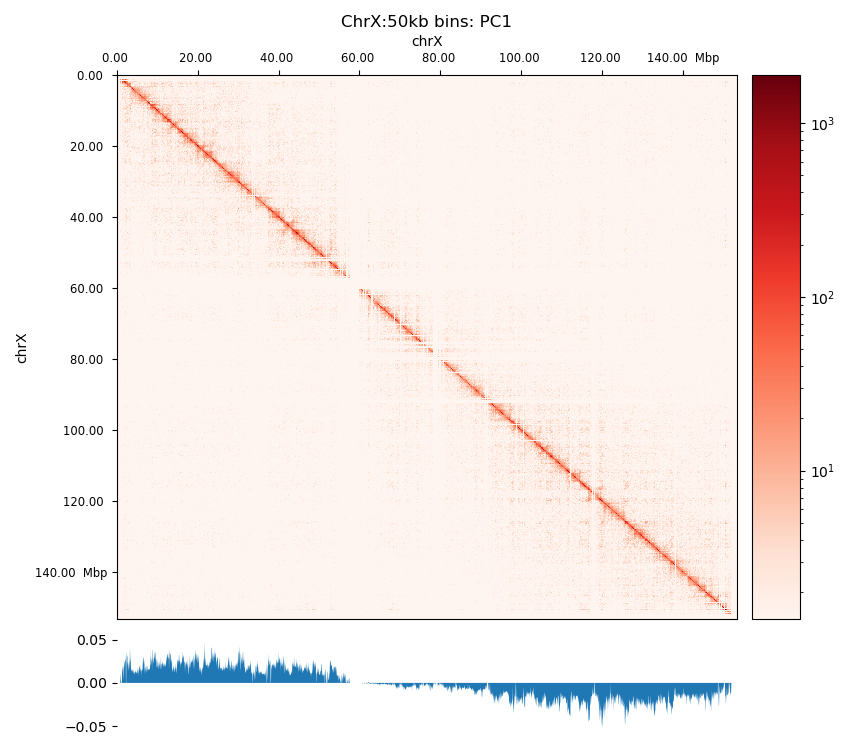
\includegraphics[keepaspectratio]{../figures/bowtie2/local/normalized/pc1_50kb_corrected_chrX.png}}

}

\subcaption{\label{fig-explorer-pc1-50kb}}

\end{minipage}%
%
\begin{minipage}{0.33\linewidth}

\centering{

\pandocbounded{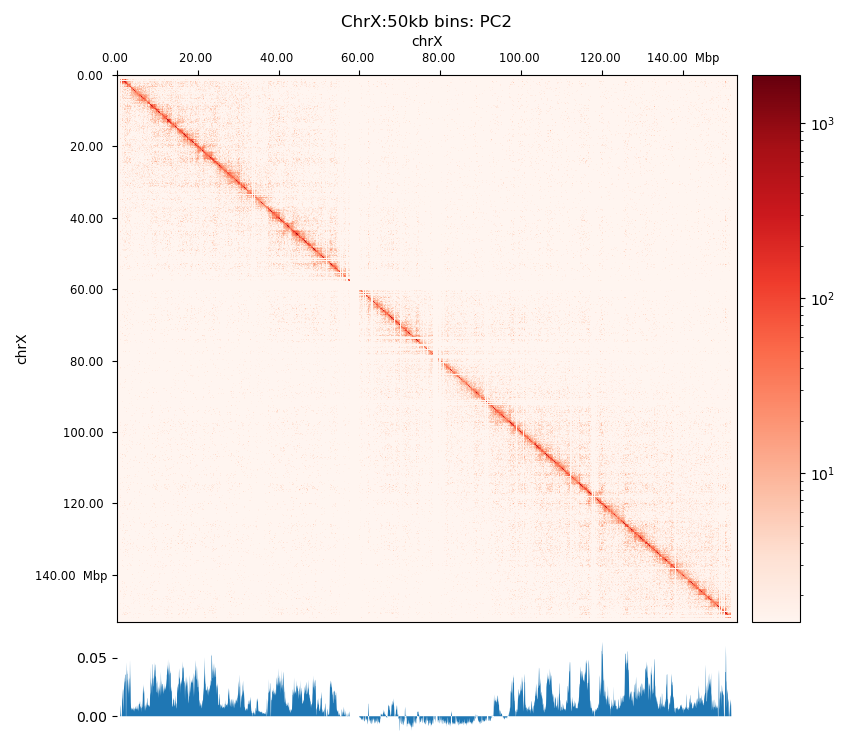
\includegraphics[keepaspectratio]{../figures/bowtie2/local/normalized/pc2_50kb_corrected_chrX.png}}

}

\subcaption{\label{fig-explorer-pc2-50kb}}

\end{minipage}%
%
\begin{minipage}{0.33\linewidth}

\centering{

\pandocbounded{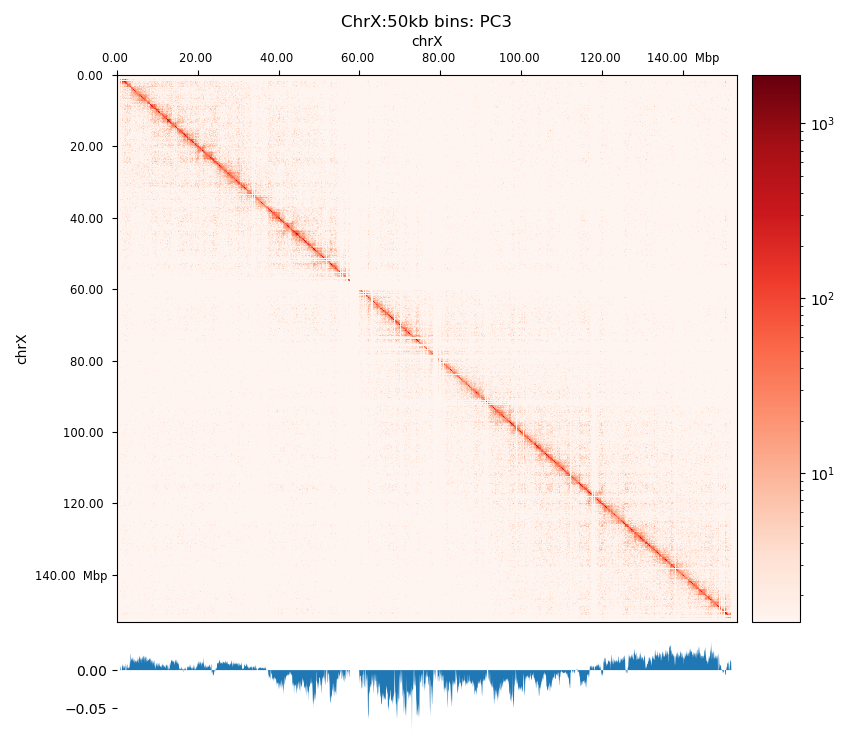
\includegraphics[keepaspectratio]{../figures/bowtie2/local/normalized/pc3_50kb_corrected_chrX.png}}

}

\subcaption{\label{fig-explorer-pc3-50kb}}

\end{minipage}%
\newline
\begin{minipage}{0.33\linewidth}

\centering{

\pandocbounded{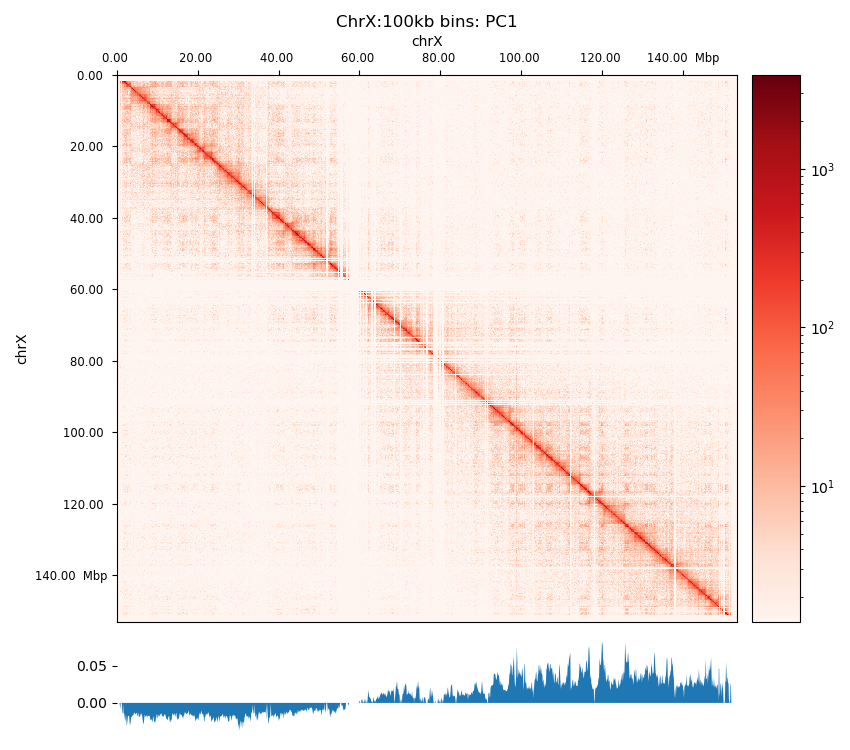
\includegraphics[keepaspectratio]{../figures/bowtie2/local/normalized/pc1_100kb_corrected_chrX.png}}

}

\subcaption{\label{fig-explorer-pc1-100kb}}

\end{minipage}%
%
\begin{minipage}{0.33\linewidth}

\centering{

\pandocbounded{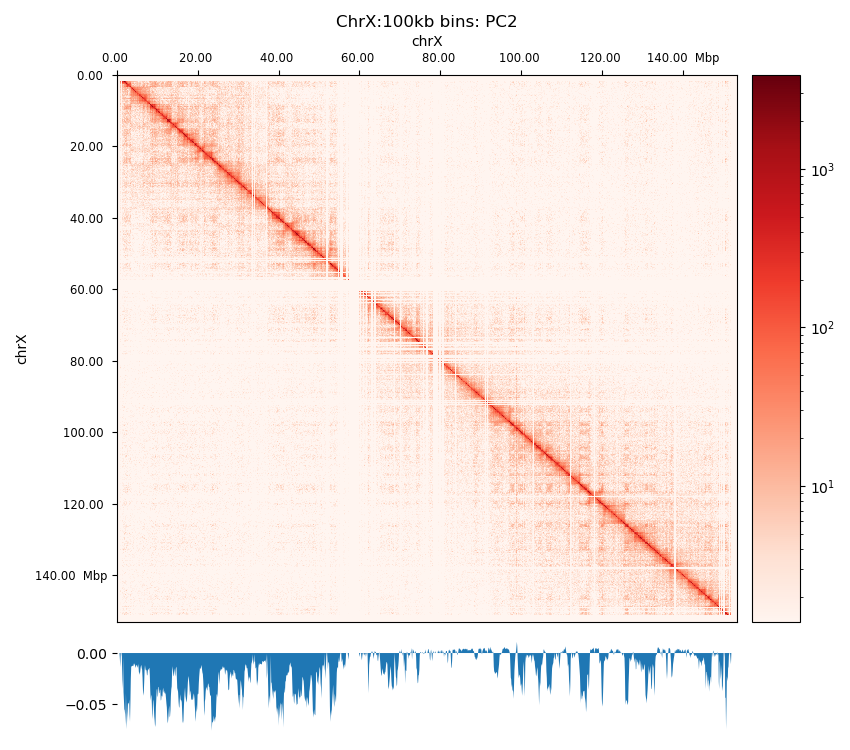
\includegraphics[keepaspectratio]{../figures/bowtie2/local/normalized/pc2_100kb_corrected_chrX.png}}

}

\subcaption{\label{fig-explorer-pc2-100kb}}

\end{minipage}%
%
\begin{minipage}{0.33\linewidth}

\centering{

\pandocbounded{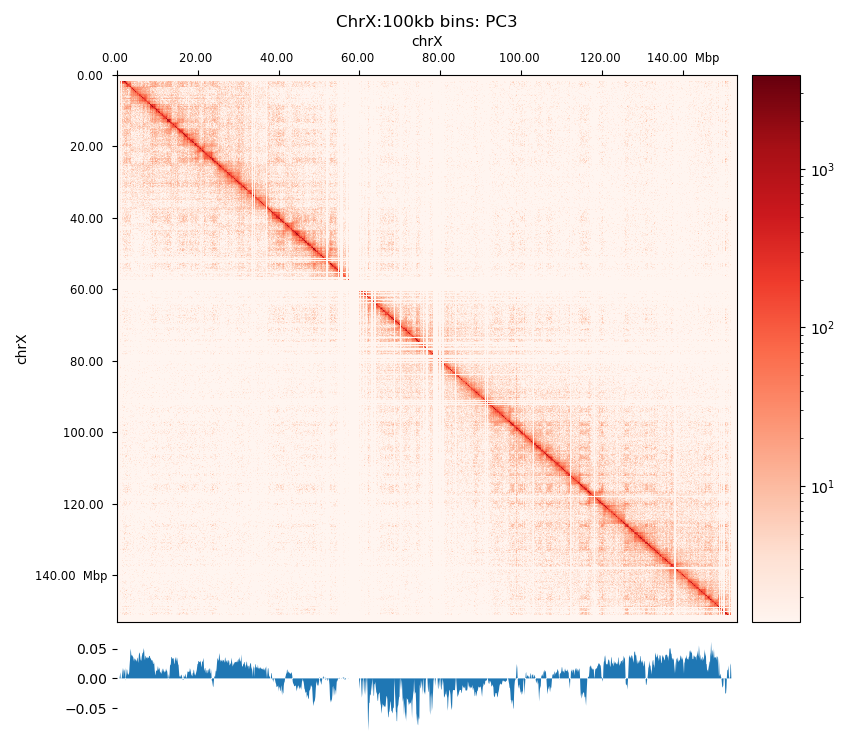
\includegraphics[keepaspectratio]{../figures/bowtie2/local/normalized/pc3_100kb_corrected_chrX.png}}

}

\subcaption{\label{fig-explorer-pc3-100kb}}

\end{minipage}%

\caption{\label{fig-explorer-pca}Corrected interaction matrix for
chromosome X along with PC1, 2, or 3, respectively. a-c: 50kb
resolution, d-f: 100kb resolution. \emph{HiCExplorer}.}

\end{figure}%

\section{Open2c ecosystem}\label{open2c-ecosystem}

\subsection{Quality Control}\label{quality-control-1}

As described, the \texttt{pairtools} module in MultiQC was used to
visualize results from \texttt{pairtools\ stats} for the two parsing
runs, see Figure~\ref{fig-pairtools-qc}. The peak at around 250 bp is a
techical artefact and should not be parsed into valid contacts.

\subsubsection{\texorpdfstring{\texttt{-\/-walks-policy\ mask}}{-\/-walks-policy mask}}\label{walks-policy-mask}

Comparing the multiQC report for each of the cell sources show similar
distributions of \emph{unmapped} (both sides unmapped), \emph{one-sided}
(one side mapped), \emph{two-sided} (both sides mapped), and
\emph{duplicated} (w.r.t. total mapped) reads. The percentage of
\emph{cis} pairs w.r.t. mapped pairs is around 70\% for all samples
(Figure~\ref{fig-pairtools-multiqc-mask-violin}). The valid pairs also
show similar distributions of pair types divided into 10 categories. The
\(P(s)\) curve looks similar for all samples as well, peaking around 250
bp separation (Figure~\ref{fig-pairtools-multiqc-mask-ps}). The QC does
not show any information about mapping quality of the reads. Note that
the \(P(s)\) curve arise from pre-filtered pairs, meaning it provides
information about the Hi-C library.

\subsubsection{\texorpdfstring{\texttt{-\/-walks-policy\ 5unique}}{-\/-walks-policy 5unique}}\label{walks-policy-5unique}

Parsing alignments with the recommended walks-policy aproximately halves
the percentage of \emph{unmapped} reads, and \emph{one-} and
\emph{two-sided} reads as well \emph{duplicated} reads are slightly
increased. Overall number of unique pairs are increased with more than
20\% increase. The percentage of \emph{cis} pairs are only decreased by
a percentage point at most
(Figure~\ref{fig-pairtools-multiqc-5unique-violin}). Changing the walks
policy does not alter the \(P(s)\) curve, meaning the parameter does not
bias the parsing w.r.t. genomic separation.

\begin{figure}

\begin{minipage}{0.50\linewidth}

\centering{

\pandocbounded{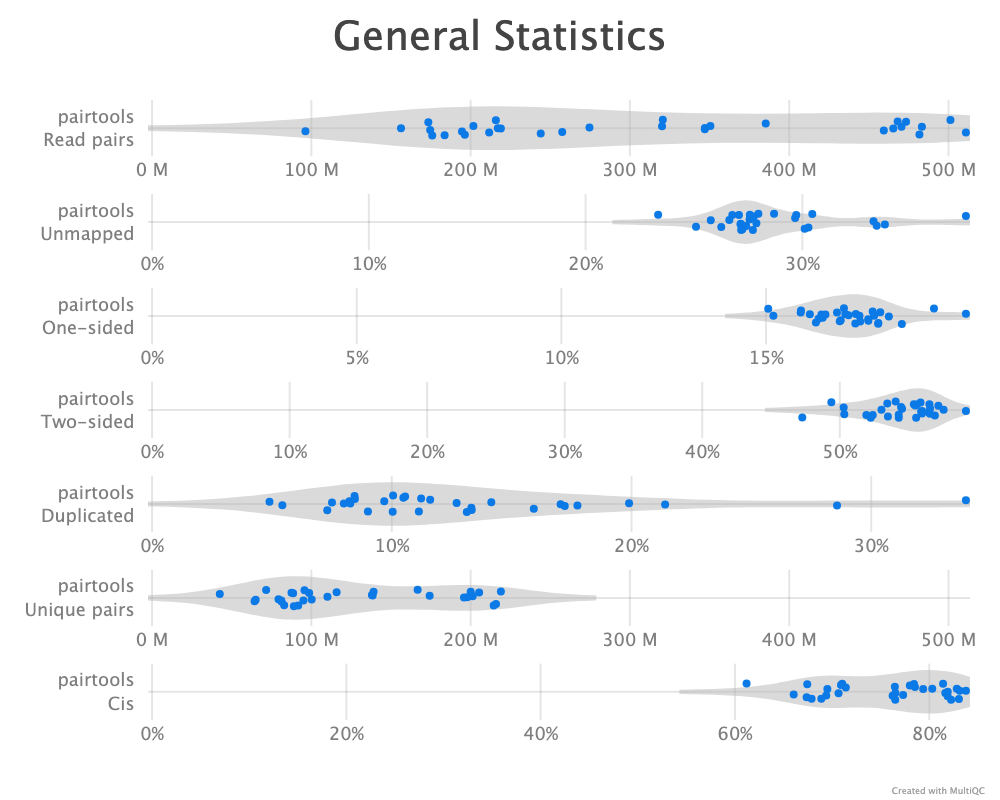
\includegraphics[keepaspectratio]{../figures/fig-pairtools-parse-multiqc-mask-violin.png}}

}

\subcaption{\label{fig-pairtools-multiqc-mask-violin}\texttt{-\/-walks-policy\ mask}}

\end{minipage}%
%
\begin{minipage}{0.50\linewidth}

\centering{

\pandocbounded{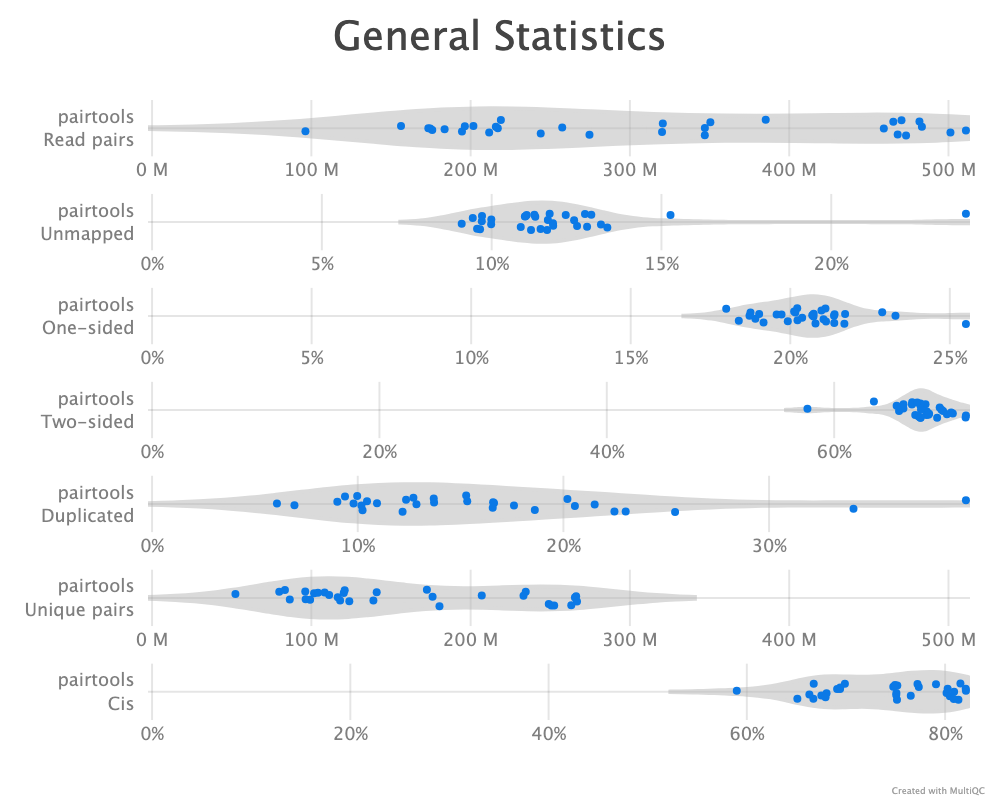
\includegraphics[keepaspectratio]{../figures/fig-pairtools-parse-multiqc-5unique-violin.png}}

}

\subcaption{\label{fig-pairtools-multiqc-5unique-violin}\texttt{-\/-walks-policy\ 5unique}}

\end{minipage}%
\newline
\begin{minipage}{0.50\linewidth}

\centering{

\pandocbounded{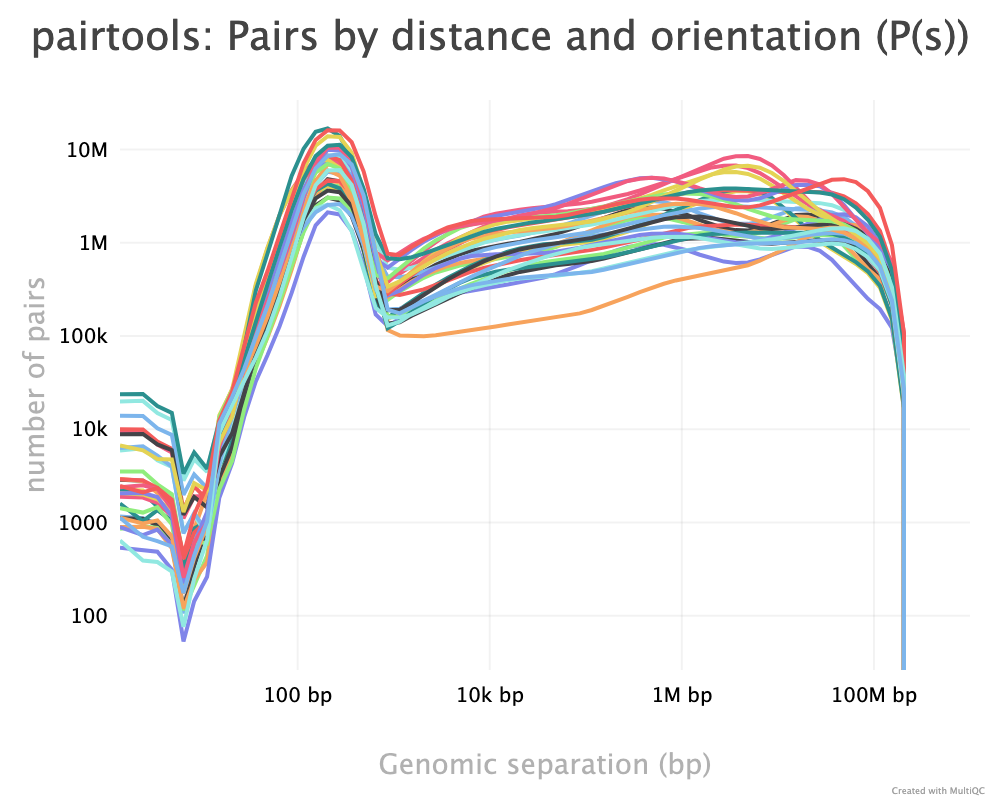
\includegraphics[keepaspectratio]{../figures/fig-pairtools-parse-multiqc-mask-ps.png}}

}

\subcaption{\label{fig-pairtools-multiqc-mask-ps}\texttt{-\/-walks-policy\ mask}}

\end{minipage}%
%
\begin{minipage}{0.50\linewidth}

\centering{

\pandocbounded{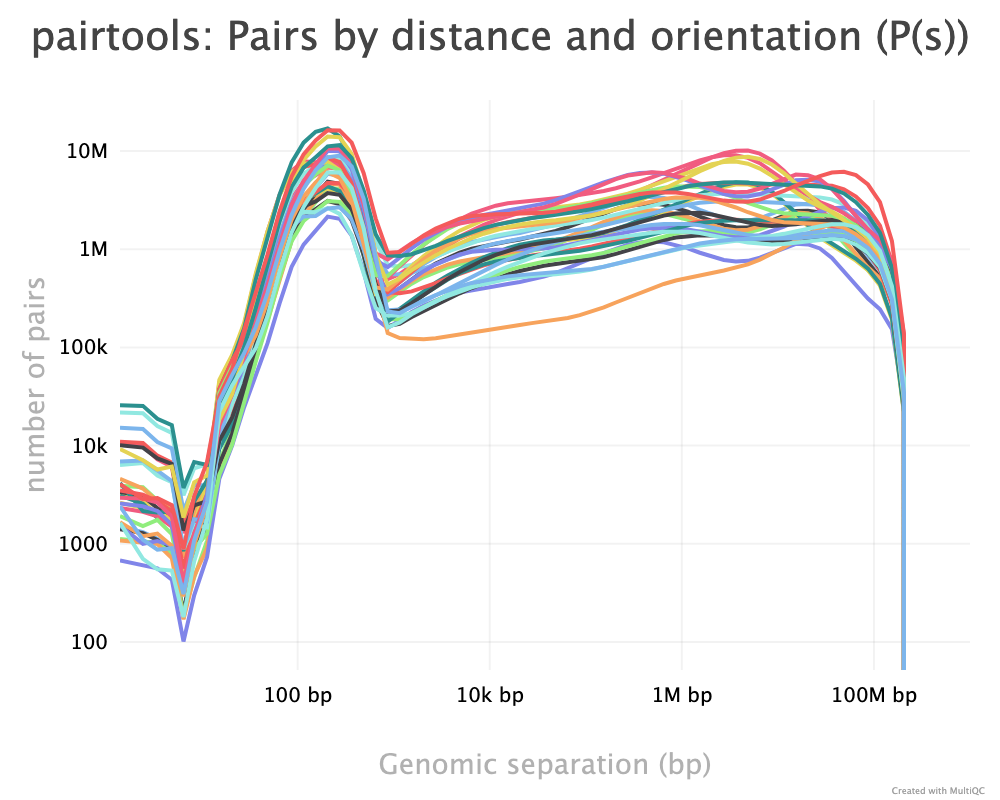
\includegraphics[keepaspectratio]{../figures/fig-pairtools-parse-multiqc-5unique-ps.png}}

}

\subcaption{\label{fig-pairtools-multiqc-5unique-ps}\texttt{-\/-walks-policy\ 5unique}}

\end{minipage}%

\caption{\label{fig-pairtools-qc}Results of \texttt{pairtools\ stats}
run on all samples from the two walks-policies. Left (a+c):
\texttt{mask}; right (b+d): \texttt{5unique}. \emph{Generated by
MultiQC} (Ewels et al. 2016). \emph{Note: X-axes are not shared in the
`Genereal Statistics' plot.}}

\end{figure}%

\subsection{Correction}\label{correction-1}

Matrix balancing did not show major improvement in the plaid pattern, as
it already showed the expected pattern. It does, however, filter out
bins that are deemed too low-count to be informative, for example
peri-centromeric regions. The matrix was expected to be smoother after
balancing (for chromosome-wide maps), as regions along a chromosome
should only vary slowly in contact frequency with other regions as they
are on a continouos molecule. Therefore, sharp contrasts represent a
sudden drop in bin count (Figure~\ref{fig-rs-chrx-raw-balanced-cgi},
raw) and should not be interpreted as devoid of interaction, but an
indication that the data is not sufficient to interpret. It is then
better to simply remove the bins instead of correcting, which will also
amplify noise. Even with a high-quality Hi-C library we expect that all
bins do not have the same coverage throughout(Lajoie, Dekker, and Kaplan
2015), as restriction enzymes do not bind equally to all regions of the
genome, and therefore, some bins will be underrepresented as an artefact
of binding/cutting efficieny of the restriction enzyme used.

We can try to mitigate the white lines of empty bins that now appear in
the matrices. The coarsegrained and interpolated matrix is useful to
make a good-looking interaction matrix, but is not that useful for
analysis purposes. It might get easier to visually inspect the matrix,
but it is not clear how well the interpolated matrix reflects the
structure of the chromatin, and it is not transparent which regions are
interpolated and which that are not. I find it purposeful for
interpolation on high-resolution (zoomed-in) views
(Figure~\ref{fig-rs-chrx-raw-balanced-cgi-subset}) with small empty
regions, but misleading for chromosome-wide maps, where typically the
centromere and extremities of the chromosome have filtered-out bins.
Interpolation is further discussed below.

The regions that are coarsegrained are small zero- or low-count bins
which are averaged, effectively reducing the resolution of those regions
until the count is sufficient. They get more frequent the longer genomic
distance (the further we travel from the diagonal), and effectively
enables us to get some intuition about the interactions. The
coarsegrain, however, does not interpolate the \texttt{NaN}s created
when filtering out whole bins in the balancing step (horisontal and
vertical lines in Figure~\ref{fig-rs-chrx-raw-balanced-cgi} and
Figure~\ref{fig-rs-chrx-raw-balanced-cgi-subset}; middle). This is done
in a subsequent step by linearly interpolating the \texttt{NaN}s.
Examining the interpolated matrix on full chrX
(Figure~\ref{fig-rs-chrx-raw-balanced-cgi}; right) gives the impression
that the pericentromeric (at \textasciitilde60 Mbp) region harbours a
\emph{very} strong compartment, but that is clearly an artefact of the
interpolation on the very large empty region of the centromere, where
the diagonal is somehow extended in a square. On the thinner lines, the
interpolation seem to be more smooth, and barely noticable on the
diagonal.

\begin{figure}[H]

\centering{

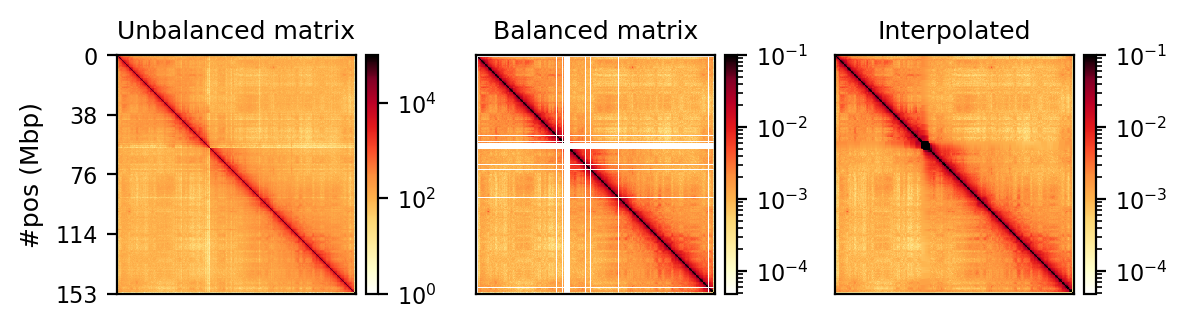
\includegraphics[width=6.17708in,height=1.70833in]{index_files/figure-latex/..-notebooks-05_rec_compartments-fig-rs-chrx-raw-balanced-cgi-output-2.png}

}

\caption{\label{fig-rs-chrx-raw-balanced-cgi}Raw, balanced, and
interpolated chrX interaction matrix in 500kb resolution. The
interpolation is done to make the matrix more visually appealing, but it
is not necessary for the analysis.}

\end{figure}%

\begin{figure}[H]

\centering{

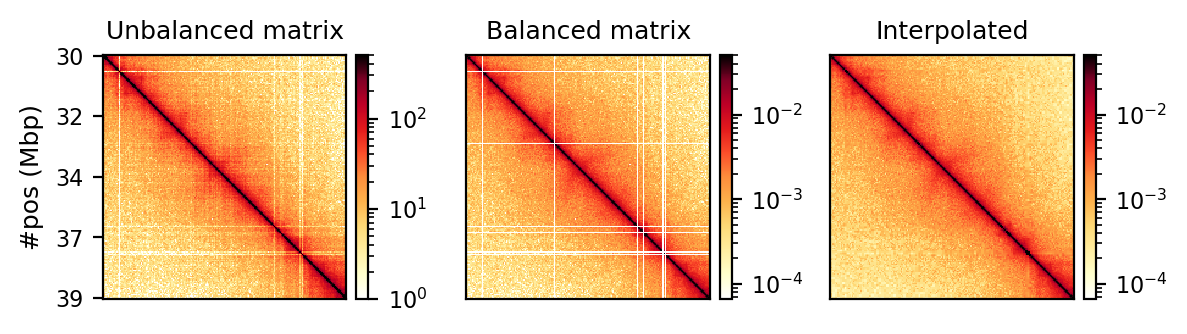
\includegraphics[width=6.17708in,height=1.73958in]{index_files/figure-latex/..-notebooks-05_rec_compartments-fig-rs-chrx-raw-balanced-cgi-subset-output-2.png}

}

\caption{\label{fig-rs-chrx-raw-balanced-cgi-subset}Raw, balanced, and
interpolated chrX interaction matrix in 50kb resolution. The
interpolation is done to make the matrix more visually appealing, but it
is not necessary for the analysis.}

\end{figure}%

\subsubsection{\texorpdfstring{\texttt{NaN}
histograms}{NaN histograms}}\label{nan-histograms}

As expected, most of the low quality bins are located on the edges of
the chromosome arms, especially the region around the centromere (Warren
et al. 2020), as they contain many repetitive sequences. The low-quality
bins are filtered out by the balancing algorithm, those bins are
\texttt{NaN} in the Hi-C matrix. The median position of the \texttt{NaN}
values (Figure~\ref{fig-e1_nan_hist}) ranges between \(58\) and
\(63.5\), which is within the estimate of the centromeric region of
\emph{rhemac10} (the UCSC browser has a continuously unannotated region
at chrX:57,500,000-60,200,000). The fact that the medians lie within the
centromeric region on all cell sources shows both that the majority of
the bad bins are in the (peri)centromeric region \emph{and} there are
approximately equally many on each side.

\begin{figure}[H]

\centering{

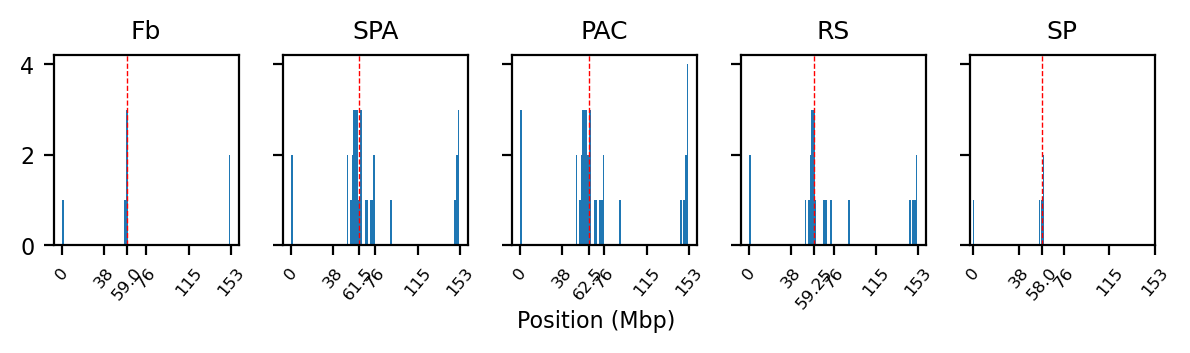
\includegraphics[width=6.19792in,height=1.83333in]{index_files/figure-latex/..-notebooks-05_rec_compartments-fig-e1_nan_hist-output-1.png}

}

\caption{\label{fig-e1_nan_hist}Histogram of NaN values in the E1
eigenvector for each cell type. Median position is marked with a red
dashed line.}

\end{figure}%

\subsection{Compartments (Eigenvectors)}\label{sec-results-eigenvectors}

The three viewframes (\emph{Full}, \emph{Arms}, \emph{10Mb}) used for
the calculation of the eigenvectors captured different variability in
the data (Figure~\ref{fig-e1-matrix-full-arms-10mb-round_spermatid}),
and as expected, the inferred compartments (colored red on the E1
tracks) are more abundant and smaller with smaller viewframes. To
determine how well each of the E1 tracks capture the pattern in the
interaction matrix, we can overlay the matrix with the E1 sign-change
and visually determine if the squares reflect the E1 sign change
(Figure~\ref{fig-e1-matrix-full-arms-10mb-round_spermatid}).

\begin{figure}

\begin{minipage}{0.50\linewidth}

\centering{

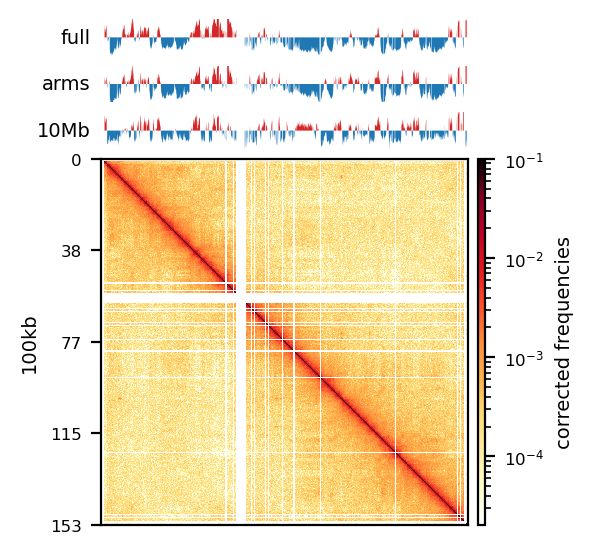
\includegraphics[width=3.09375in,height=2.88542in]{index_files/figure-latex/..-notebooks-07_various_plotting-fig-e1-matrix-full-arms-10mb-round_spermatid-output-1.png}

}

\subcaption{\label{fig-e1-matrix-full-arms-10mb-round_spermatid-1}100kb
resolution}

\end{minipage}%
%
\begin{minipage}{0.50\linewidth}

\centering{

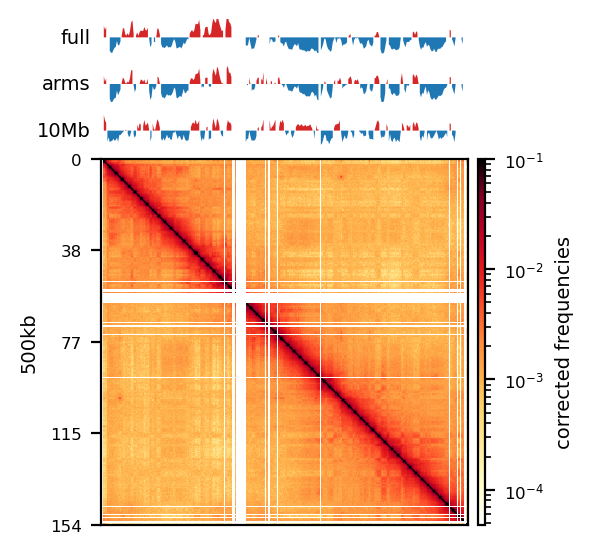
\includegraphics[width=3.09375in,height=2.88542in]{index_files/figure-latex/..-notebooks-07_various_plotting-fig-e1-matrix-full-arms-10mb-round_spermatid-output-2.png}

}

\subcaption{\label{fig-e1-matrix-full-arms-10mb-round_spermatid-2}500kb
resolution}

\end{minipage}%

\caption{\label{fig-e1-matrix-full-arms-10mb-round_spermatid}E1
eigenvector values for merged round spermatid samples at a) 100kb or b)
500kb resolution, as well as the interaction matrix. E1 was restricted
to either Full-chromosome (top), Chromosome-arms (middle), or 10Mb
windows (bottom)}

\end{figure}%

I decide that without more finescaled knowledge than the position of the
centromeres, the arbitrary size of the 10 Mb windowed E1 can not fully
be justified. That is, we could arbitrarily calculate any windowed E1
track. Also, Wang et al. (2019) concludes only for pachytene
spermatocyte to show local interactions in the 10Mb viewframe (what they
refer to as \emph{refined A/B-compartments}), and all the other stages
of spermatogenesis were consistent with the conventional A/B
compartments. The reasonable thing to do is therefore to continue the
analysis, focusing on the arms-restricted eigendecomposition.
Nevertheless, we also keep \emph{refined} compartments in the analysis.

\begin{figure}

\begin{minipage}{0.05\linewidth}
~\end{minipage}%
%
\begin{minipage}{0.46\linewidth}

\centering{

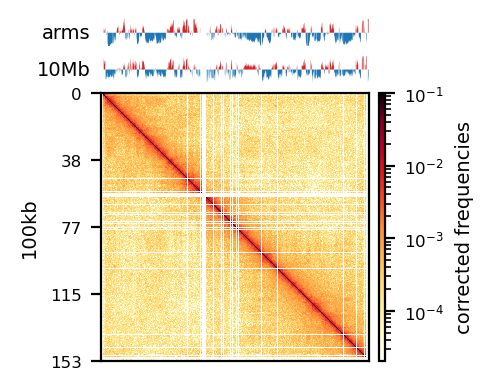
\includegraphics[width=2.57292in,height=2.03125in]{index_files/figure-latex/..-notebooks-07_various_plotting-fig-rs100-recpe-pe-output-1.png}

}

\subcaption{\label{fig-rs100-recpe-pe-1}\texttt{5unique}:
chrX:start-end}

\end{minipage}%
%
\begin{minipage}{0.46\linewidth}

\centering{

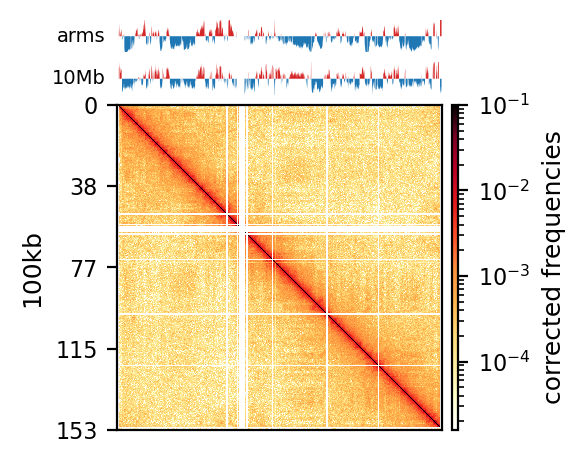
\includegraphics[width=2.57292in,height=2.03125in]{index_files/figure-latex/..-notebooks-07_various_plotting-fig-rs100-recpe-pe-output-2.png}

}

\subcaption{\label{fig-rs100-recpe-pe-2}\texttt{mask}: chrX:start-end}

\end{minipage}%
%
\begin{minipage}{0.05\linewidth}
~\end{minipage}%
\newline
\begin{minipage}{0.05\linewidth}
~\end{minipage}%
%
\begin{minipage}{0.46\linewidth}

\centering{

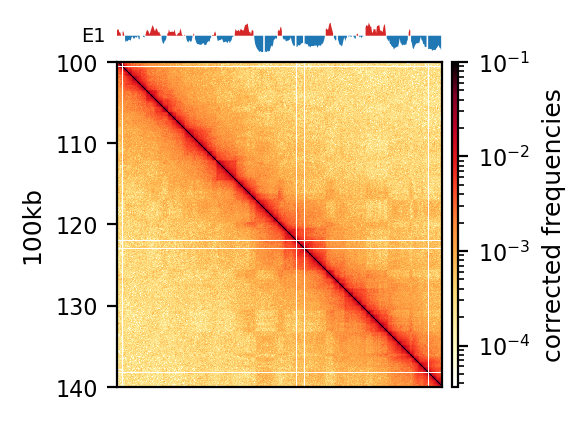
\includegraphics[width=2.57292in,height=2.09375in]{index_files/figure-latex/..-notebooks-07_various_plotting-fig-rs100-recpe-pe-output-3.png}

}

\subcaption{\label{fig-rs100-recpe-pe-3}\texttt{5unique}:
chrX:70Mb-78Mb}

\end{minipage}%
%
\begin{minipage}{0.46\linewidth}

\centering{

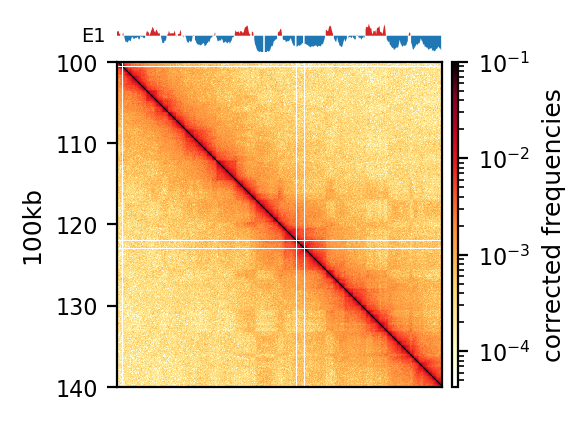
\includegraphics[width=2.57292in,height=2.09375in]{index_files/figure-latex/..-notebooks-07_various_plotting-fig-rs100-recpe-pe-output-4.png}

}

\subcaption{\label{fig-rs100-recpe-pe-4}\texttt{mask}: chrX:70Mb-78Mb}

\end{minipage}%
%
\begin{minipage}{0.05\linewidth}
~\end{minipage}%

\caption{\label{fig-rs100-recpe-pe}Round Spermatid (RS) at 100kb,
comparing the impact of parsing parameters}

\end{figure}%

Additionally, as I created coolers with two different sets of parsing
parameters we will compare the resulting matrices and their compartments
(Figure~\ref{fig-rs100-recpe-pe}). As expected, we observe more empty
bins in the Hi-C matrix when comparing the initial run (\texttt{mask})
to the recommended parameters (\texttt{5unique}), but otherwise, the
interaction pattern is indestinguishable. The effect on the E1 is more
noticable, where the absolute magnitude of the E1 values is generally
smaller. There is, however, a small region that changes sign (from A to
B) on the 10Mb-windowed (`refined') E1 track
(Figure~\ref{fig-rs100-recpe-pe};c+d). This region is surrounded by
added empty bins, which could mean that too many low quality pairs in
\texttt{mask} were introducing bias and swapped the sign of E1. It is
supported by the fact that the sign change \emph{only} occured in
\emph{refined} E1, and that the sign after filtering weak pairs
(\(mapq < 30\)) is consistent with the \emph{arms} view. It supports my
previous postulate that it is better to use a viewframe with explicit
molecular meaning than one of an arbitrary window size. That said, the
\texttt{mapq} threshold should really be determined taking both coverage
and resolution into account. For our purposes, and with the \emph{arms}
view, the mapping- and parsing parameters do not seem to be too
sensitive.

To emphasize the findings, the sets of A-compartments were compared
between the two parsing runs, showing almost identical compartment
calls. Additionally, the set difference was 8 bins between PE and recPE
for round spermatid 100kb and 5 bins for fibroblast for \emph{arms}
viewframe (Figure~\ref{fig-rs-fb-100-pe-recpe-intervals}; a+b,
respectively). We observe a high number of differences around 76Mb for
the refined compartments (10Mb) of round spermatid, which is consistent
with the sign-flip of E1 values discussed earlier. Anything else would
be surprising, as it is the same data, but visualized in a different
way.

\begin{figure}

\begin{minipage}{0.10\linewidth}
~\end{minipage}%
%
\begin{minipage}{0.40\linewidth}

\centering{

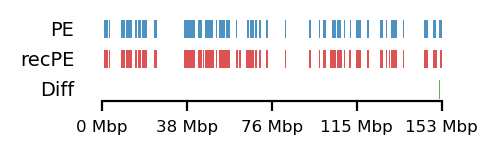
\includegraphics[width=2.59375in,height=0.80208in]{index_files/figure-latex/..-notebooks-07_various_plotting-fig-rs-fb-100-pe-recpe-intervals-output-1.png}

}

\subcaption{\label{fig-rs-fb-100-pe-recpe-intervals-1}RS: arms}

\end{minipage}%
%
\begin{minipage}{0.40\linewidth}

\centering{

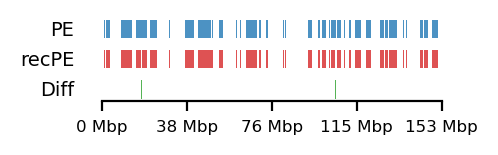
\includegraphics[width=2.59375in,height=0.80208in]{index_files/figure-latex/..-notebooks-07_various_plotting-fig-rs-fb-100-pe-recpe-intervals-output-2.png}

}

\subcaption{\label{fig-rs-fb-100-pe-recpe-intervals-2}Fib: arms}

\end{minipage}%
%
\begin{minipage}{0.10\linewidth}
~\end{minipage}%
\newline
\begin{minipage}{0.10\linewidth}
~\end{minipage}%
%
\begin{minipage}{0.40\linewidth}

\centering{

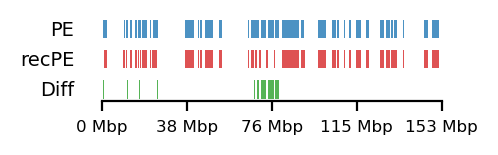
\includegraphics[width=2.59375in,height=0.80208in]{index_files/figure-latex/..-notebooks-07_various_plotting-fig-rs-fb-100-pe-recpe-intervals-output-3.png}

}

\subcaption{\label{fig-rs-fb-100-pe-recpe-intervals-3}RS: 10Mb}

\end{minipage}%
%
\begin{minipage}{0.40\linewidth}

\centering{

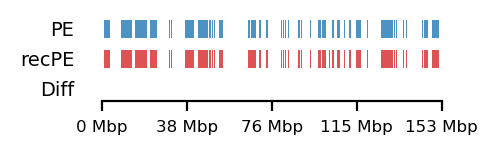
\includegraphics[width=2.59375in,height=0.80208in]{index_files/figure-latex/..-notebooks-07_various_plotting-fig-rs-fb-100-pe-recpe-intervals-output-4.png}

}

\subcaption{\label{fig-rs-fb-100-pe-recpe-intervals-4}Fib: 10Mb}

\end{minipage}%
%
\begin{minipage}{0.10\linewidth}
~\end{minipage}%

\caption{\label{fig-rs-fb-100-pe-recpe-intervals}Round Spermatid (RS)
and Fibroblast (Fb) at 100kb, comparing the impact of parsing parameters
on A-compartment calling at different viewframes; \emph{arms},
\emph{10Mb}. PE: initial parse (masking complex walks); recPE:
recommended parse (reporting the 5'most unique alignment of a complex
walk).}

\end{figure}%

The observed difference between the sets can for our data be attributed
to chance, but we cannot draw general conclusions about the parameters
in general. I argue that the quality and size of the Hi-C library will
influence sensitive to parsing parameters. In that case, the most
flexible approach is still to follow the recommendations from
\texttt{cooler} to report more pairs as valid contacts, and then create
coolers with different \emph{mapq} filters if issues are encountered.

\section{Comparing Genomic Intervals}\label{comparing-genomic-intervals}

The comparison of genomic intervals was modified along the way, as we
gained more knowledge and caught mistakes in the original implementation
(especially of the proxomity test). Here, I only report the results of
the final version of the software, but the modifications and
implications hereof are discussed in Section~\ref{sec-discussion}.

\subsection{Compartment Edges (transition
zones)}\label{compartment-edges-transition-zones}

We compare how the ECH90 regions fit when queried on top of the
A-compartments and equivalently for the edges, for fibroblasts and round
spermatids at 100kb resolution. When queried against the edges instead,
the the total set size is reduced to less than 50\%. Interestingly, some
of the intersections between A-compartments and ECH90 remain, and new
ones appear as we move to the outside edge of the compartment
(Figure~\ref{fig-comps-edges-ech}). This indicates that most, but not
all, of the intersection between ECH90 regions and the A-compartments
are within 100kb of the compartment edge, and additional overlap is
gained if we define a transition zone on the outside of the edge as
well. To visualize this (outside) edge enrichment, we find the set
difference of the ECH-intersection to compartments and edges,
respectively (Figure~\ref{fig-edge-enrichment}), thus removing all the
`inside' edges. We observe that in almost all of the of the regions of
\(ECH \cap Comp\) are accompanied by an edge also intersecting ECH
(\(ECH \cap Edge\)), localized where the \emph{Diff} track aligns
(within 100kb) with both \(CompInt\) and \(EdgeInt\).

\begin{figure}

\begin{minipage}{0.01\linewidth}
~\end{minipage}%
%
\begin{minipage}{0.49\linewidth}

\centering{

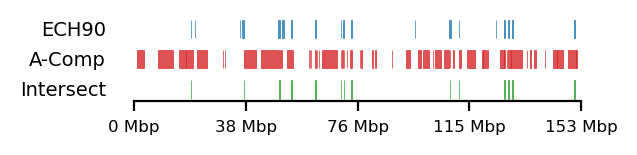
\includegraphics[width=3.3125in,height=0.80208in]{index_files/figure-latex/..-notebooks-07_various_plotting-fig-comps-edges-ech-output-1.png}

}

\subcaption{\label{fig-comps-edges-ech-1}Fibroblast A-compartments}

\end{minipage}%
%
\begin{minipage}{0.49\linewidth}

\centering{

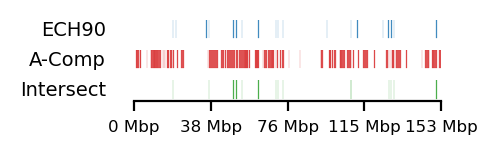
\includegraphics[width=3.3125in,height=0.80208in]{index_files/figure-latex/..-notebooks-07_various_plotting-fig-comps-edges-ech-output-2.png}

}

\subcaption{\label{fig-comps-edges-ech-2}Round Spermatid A-compartments}

\end{minipage}%
%
\begin{minipage}{0.01\linewidth}
~\end{minipage}%
\newline
\begin{minipage}{0.01\linewidth}
~\end{minipage}%
%
\begin{minipage}{0.49\linewidth}

\centering{

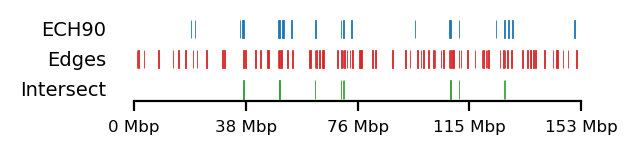
\includegraphics[width=3.3125in,height=0.80208in]{index_files/figure-latex/..-notebooks-07_various_plotting-fig-comps-edges-ech-output-3.png}

}

\subcaption{\label{fig-comps-edges-ech-3}Fibroblast edges}

\end{minipage}%
%
\begin{minipage}{0.49\linewidth}

\centering{

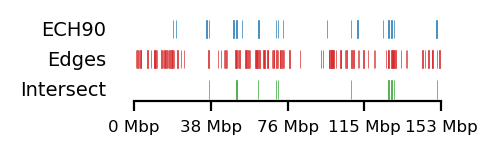
\includegraphics[width=3.3125in,height=0.80208in]{index_files/figure-latex/..-notebooks-07_various_plotting-fig-comps-edges-ech-output-4.png}

}

\subcaption{\label{fig-comps-edges-ech-4}Round Spermatid edges}

\end{minipage}%
%
\begin{minipage}{0.01\linewidth}
~\end{minipage}%

\caption{\label{fig-comps-edges-ech}Visual representation of the genomic
intervals of ECH90, A-compartments (a+b), edges (c+d), and their
intersections. Shown fibroblast (a+c) and round spermatid (b+d) at 100kb
resolution and arms viewframe.}

\end{figure}%

\begin{figure}

\begin{minipage}{0.01\linewidth}
~\end{minipage}%
%
\begin{minipage}{0.49\linewidth}

\centering{

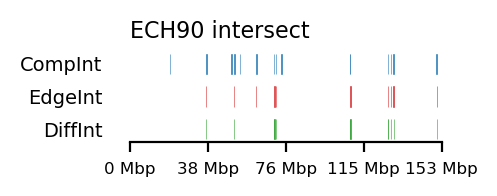
\includegraphics[width=3.3125in,height=1.02083in]{index_files/figure-latex/..-notebooks-07_various_plotting-fig-edge-enrichment-output-1.png}

}

\subcaption{\label{fig-edge-enrichment-1}Round Spermatid}

\end{minipage}%
%
\begin{minipage}{0.49\linewidth}

\centering{

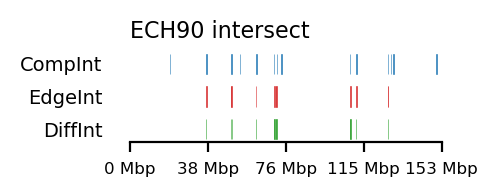
\includegraphics[width=3.3125in,height=1.02083in]{index_files/figure-latex/..-notebooks-07_various_plotting-fig-edge-enrichment-output-2.png}

}

\subcaption{\label{fig-edge-enrichment-2}Fibroblast}

\end{minipage}%
%
\begin{minipage}{0.01\linewidth}
~\end{minipage}%

\caption{\label{fig-edge-enrichment}Visual representation of the
enrichment of edges in the intersection of ECH90 and A-compartments.
Shown round spermatid (a) and fibroblast (b) at 100kb resolution and
arms viewframe. Note that the edge-regions are too small to be
distinguished visually from the compartment on the graph, making it look
like they overlap, even though the difference is reported.}

\end{figure}%

I apply both the proximity and Jaccard test to see how well the
observations could be explained by chance. For completeness, the tests
are performed for all cell types, but only use 100kb resolution and arms
viewframe. We observe that both fibroblast and round spermatids have
significant overlap (Jaccard p-values \(0.012\) and \(0.010\),
respectively), meaning the edge zone have more intersection with the ECH
regions than expected by chance. None of the samples passed the
proximity test, meaning the non-overlapping segments were no more
proximal than expected by chance. A significant proximity test (when
performed on the edges) might provide information about the potential of
expanding or moving the transition window. That is, if the
non-overlapping regions are \emph{very} proximal, a larger (or shifted)
window to only capture the 200kb region outside of the edge might be
favourable. With the very small amount of observed proximity (high
p-values), we might consider shrinking the windows.

\subsection{Testing against regions of selection in
baboons}\label{testing-against-regions-of-selection-in-baboons}

The data for this analysis was provided by Kasper Munch in bed-like
format, mapped to \emph{panu\_3.0} (PapAnu4) assembly. The intervals
define genomic regions in a hybrid/migrating population of baboon where
strong negative selection acts against minor parent ancestry (Sørensen
et al. 2023). The segments had to be lifted to \emph{rheMac10}
coordinates to be able to correlate the two sets of intervals. The
original UCSC-liftOver (Hinrichs 2006) is very strict and does not try
to conserve segments in favor of accuracy e.g.~inversions or small
indels, which results in highly fragmented regions when lifted to
another assembly, if the segments are not continouos on the new
assembly. For our analysis, it is not the exact genomic position or
order of sub-genic regions that are important, but rather, the start and
end coordinates of each segment are quantified. To favor preservation of
segments, we use \emph{segment\_liftover} (Gao, Huang, and Baudis 2018),
resulting in much more similar segments to the original
(Figure~\ref{fig-compare-liftover}). As no chain file from
\emph{panu\_3.0} to \emph{Mmul\_10} was available, we used
\emph{panu\_2.0} as intermediate.

\begin{figure}[H]

\centering{

\centering{

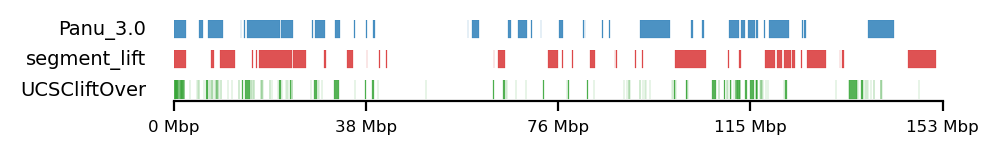
\includegraphics[width=6.23958in,height=0.80208in]{index_files/figure-latex/..-notebooks-07_various_plotting-fig-compare-liftover-output-1.png}

}

\subcaption{\label{fig-compare-liftover-1}high-olive}

\centering{

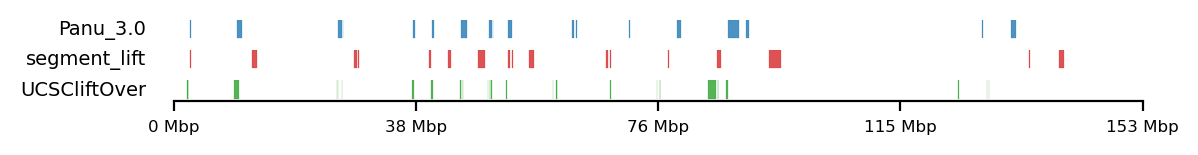
\includegraphics[width=6.23958in,height=0.80208in]{index_files/figure-latex/..-notebooks-07_various_plotting-fig-compare-liftover-output-2.png}

}

\subcaption{\label{fig-compare-liftover-2}high-hama}

}

\caption{\label{fig-compare-liftover}Comparison of a) high-olive and b)
high-hama intervals between Panu\_3.0, segment\_liftover, or UCSC
liftOver coordinates when lifting from
PapAnu4--\textgreater PapAnu3--\textgreater rheMac10.}

\end{figure}%

Initially, the compartment edges of round spermatid at 100kb resolution
(RS100) were plotted against the lifted coordinates from the baboon
hybrid population, where either all the sampled individuals have olive
(\emph{P. anubis}) ancestry or 95\% of the sampled individuals have
hamadryas (\emph{P. hamadryas} ancestry. Their respective intersections
were plotted underneath. We expect less intersection for
\emph{hamadryas} than for \emph{anubis} as the total set size is much
smaller. The compartment edges and \emph{Papio anubis}-derived
regions(Figure~\ref{fig-baboon-rs100-intersect}; b) seem to be highly
enriched in the first 25 Mbp, and thus it has a high degree of
intersection with the compartment edges. Interestingly, the ECH90 set is
nearly empty in that region, which could be useful for determining the
mechanism for selecting against the \emph{P.hamadryas} ancestral allele
in the hybrid baboon population. The \emph{P.hamadryas}-derived regions
seem intersect the compartment edges more centered on the chromosome
(Figure~\ref{fig-baboon-rs100-intersect}; a). The proximity test
initially ruled out that the non-intersecting parts of the respective
regions were this proximal by chance. However, after updating the method
to exclude whole segments that partially overlaps (instead of keeping
their non-overlapping parts), there was no statistical significance.
Additionally, the Jaccard test revealed that the intersection between
the RS100 and both Hi-\emph{P.hama} and Hi-\emph{P.anu} can be explained
by chance alone with no p-values below \(0.05\).

\begin{figure}

\begin{minipage}{0.01\linewidth}
~\end{minipage}%
%
\begin{minipage}{0.49\linewidth}

\centering{

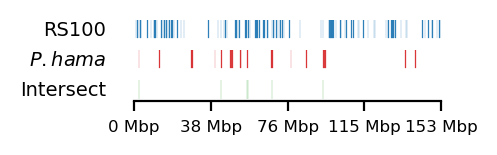
\includegraphics[width=3.3125in,height=0.80208in]{index_files/figure-latex/..-notebooks-07_various_plotting-fig-baboon-rs100-intersect-output-1.png}

}

\subcaption{\label{fig-baboon-rs100-intersect-1}\emph{P. hamadryas} +
arms E1}

\end{minipage}%
%
\begin{minipage}{0.49\linewidth}

\centering{

\includegraphics[width=3.3125in,height=0.80208in]{index_files/figure-latex/..-notebooks-07_various_plotting-fig-baboon-rs100-intersect-output-2.png}

}

\subcaption{\label{fig-baboon-rs100-intersect-2}\emph{P. anubis} + arms
E1}

\end{minipage}%
%
\begin{minipage}{0.01\linewidth}
~\end{minipage}%
\newline
\begin{minipage}{0.01\linewidth}
~\end{minipage}%
%
\begin{minipage}{0.49\linewidth}

\centering{

\includegraphics[width=3.3125in,height=0.80208in]{index_files/figure-latex/..-notebooks-07_various_plotting-fig-baboon-rs100-intersect-output-3.png}

}

\subcaption{\label{fig-baboon-rs100-intersect-3}\emph{P. hamadryas} +
10Mb E1}

\end{minipage}%
%
\begin{minipage}{0.49\linewidth}

\centering{

\includegraphics[width=3.3125in,height=0.80208in]{index_files/figure-latex/..-notebooks-07_various_plotting-fig-baboon-rs100-intersect-output-4.png}

}

\subcaption{\label{fig-baboon-rs100-intersect-4}\emph{P. anubis} + 10Mb
E1}

\end{minipage}%
%
\begin{minipage}{0.01\linewidth}
~\end{minipage}%

\caption{\label{fig-baboon-rs100-intersect}Comparing the A-compartment
edges of round spermatid (RS) with regions in baboons from hybrid
population where a) 95\% of sampled individuals have \emph{Papio
hamadryas} ancestry or b) 100\% of the samples have \emph{Papio anubis}
ancestry. The regions are extracted and lifted from PapAnu4 to rhemac10
using segment\_liftover.}

\end{figure}%

\subsection{Testing limits}\label{testing-limits}

We then abandoned the idea of a 200kb transition zone between the
compartments. It was introduced as a less stringent edge, allowing the
intersection of the selected regions to be within a defined threshold.
We hoped a weaker threshold could allow for more variance, but it turned
out to be the opposite (Table~\ref{tbl-svedig-tabel-significant}). After
defining the compartment limits (\texttt{\_edge\_1bp}), we perform tests
on combinations of all five sources (fibroblast, spermatogonia,
pachytene spermatocyte, round spermatid, sperm) and 2 viewframes (arms,
10Mb) and 5 queries. The queries were modified as such; the full ECH was
used unmodified for the tests as it was already shown to overlap
(Jaccard) fibroblast and round spermatid. \emph{hama} and \emph{olive}
limits were used separately and as a concatenated set
(\texttt{hamaolive\_edge\_1pb}), to increase the effect size, especially
as the \emph{hama} set is quite small compared to the rest of the sets.
By their definition, \emph{olive} and \emph{hama} do not overlap, and
can safely be concatenated (see
Figure~\ref{fig-introduce-selected-regions} for confirmation). Now, we
observe significant p-values across all cell types.

Reassuringly, both fibroblast and round spermatid still have significant
Jaccard p-values for the arms viewframe although the p-values have
increased (to \(0.017\) and \(0.028\), respectively). Now, all tissues
except sperm show significant overlap with ECH regions, especially
spermatogonia and pachytene spermatocytes with p-values \(0.006\) and
\(0.005\), respectively. Only fibroblast and spermatogonia significantly
overlap the ECH region for both viewframes, indicating that their
predicted compartments shift only minimally compared to the pachytene
spermatocyte and round spermatid when narrowing the viewframe. Pachytene
spermatocyte and round spermatid loose their significance when narrowing
the viewframe, meaning their compartments are highly varied between the
two views, and the same conclusion can be drawn about sperm, as it gains
significance when the viewframe is narrowed. Interestingly, only sperm
overlaps the baboon regions with olive ancestry, and no tissue overlaps
with hamadryas ancestry. Conversely, when concatenating the olive and
hamadryas sets to capture all selection in baboons, both spermatogonia,
pachytene spermatocyte, and sperm are significantly proximal. Here,
sperm, which is not proximal in the arms viewframe, has the lowest
p-value (\(p=0.001\)).

\begin{longtable}[]{@{}llllllll@{}}

\caption{\label{tbl-svedig-tabel-significant}Test results from proximity
and Jaccard, comparing ECH (full regions) or baboon 1bp limits with
compartment 1bp limits from all cell types. Significant p-values across
tissue types. All insignificant p-values are filtered out. \emph{Fb:
Fibroblast, Spa: Spermatogonia, Pac: Pachytene Spermatocyte, RS: Round
Spermatid, Sperm: Sperm}}

\tabularnewline

\caption{}\label{T_a1cfd}\tabularnewline
\toprule\noalign{}
View & Query & Test & Fb & Spa & Pac & RS & Sperm \\
\midrule\noalign{}
\endfirsthead
\toprule\noalign{}
View & Query & Test & Fb & Spa & Pac & RS & Sperm \\
\midrule\noalign{}
\endhead
\bottomrule\noalign{}
\endlastfoot
10Mb & ECH90 & jaccard & 0.021460 & 0.006110 & - & - & 0.047500 \\
10Mb & olive\_1bp & proximity & - & - & - & - & 0.016140 \\
10Mb & olivehama\_1bp & proximity & - & 0.018790 & 0.012300 & - &
0.001280 \\
arms & ECH90 & jaccard & 0.016560 & 0.006120 & 0.005340 & 0.027690 &
- \\
arms & olivehama\_1bp & proximity & - & - & 0.035640 & - & - \\

\end{longtable}

\newpage{}

\chapter{Discussion}\label{sec-discussion}

\section{On Reproducibility}\label{on-reproducibility}

As an extensive reproducibility infrastructere became a major part of
the project, I have to reflect upon the advantages it has, but also the
consequences it inevitably brings along. First, reproducibility is the
basis of scientific progression, and idealisticly it should come before
the discovery itself. But let us not pretend that reproducibility is
favored above hypothesis testing to be the driving forces of
progression, and let us not pretend that it has a singular definition.
There are many layers to reproducibility, and we do, of course, not need
to host a website or to construct a single-command pipeline for
reproducing the analysis to call a study \emph{reproducible}.
Additionally, the option only exist for analyses that are strictly
computational. It is, however, very useful and can greatly improve
downstream efficiency, and I find it important to at least explore the
available options. If such a pipeline had existed, I would not have had
to spend weeks to update the results of Wang et al. (2019) to reflect a
more recent reference genome. With such a pipeline, it is now easy to
extend the analysis to include more samples and other species.
Additionally, if they had made the coordinates of the compartments
available, I could probably have used them directly and start by
comparing genomic intervals. Instead, this became a study more of Hi-C
data analysis than comparing genomic intervals.

At the time of writing, the repository is \emph{almost there} w.r.t.
reproducibility, but still not quite. It only reproduces the final
analysis done with \emph{bwa}, \emph{pairtools}, \emph{cooler},
\emph{cooltools}, and not the preliminary analyses comparing aligners
and using \emph{HicExplorer}. This is the intention, as most use-cases
would not need the results of a preliminary methodological comparison.
However, the workflows are saved under \texttt{scripts/} and can be run
from there, or they can be added to the main \texttt{workflow.py} as
separate targets. A small amount of refactoring of the directory
structure is required as well, because some files are fetched from a
parent folder to the project directory. Additionally, the main workflow
is intensive in I/O and could be heavily optimized by piping between
commands instead of writing the outputs to file and reading the files
from the next command. However, that would make it harder to debug, as
no checkpoints are saved. It would not be as efficient use of resources,
which are requested on target level, as the analysis would have to run
as a single target. The different steps of the pipeline are either
CPU-bound or RAM-bound, but rarely both, and it would take some
experimenting to find the optimal compromise. Additionally, the
computational steps between a raw \emph{.cool} file and a balanced,
multi-resolution \emph{.mcool} are performed in a notebook, and the
steps should be moved to the workflow. Then, a final target should be
added to the workflow, executing all the notebooks (they are named in
order), to generate the figures and tables that are used in this
manuscript and on the main project pages.

There is a major downside when trying to conform to an idealistic
framework---the generation of figures and tables. Throughout this
project, I have adhered to the rule that none of the figures and tables
should be created or even annotated manually. It is very time-consuming
to create production-quality figures that needs no further enhancements
before embedding into a manuscript, and even more so do create tables
that are both compatible with HTML and PDF. Here, Quarto inherits the
limitations of Pandoc (which it uses internally to convert Markdown to
its output formats), and it does not work well with complex grouped
tables generated in Python to translate into LaTeX (which again is an
idealistic typesetting system). As Quarto is a relatively new framework
(first release 2022-07-28 Quarto Team (2022)), there are contiously
released updates to fix bugs. Therefore, one can spend hours on a
workaround for a feature, which could be included in week's release.

I believe it is an important exercise to force oneself to be cautious
about design choices and explore the advantages and limitations of the
tools we have available to communicate what we want to communicate.

\section{On Methodology}\label{on-methodology}

HiCExplorer is a comprehensive software that consist of an extensive
list of ready-made command line functions that calls Python source code.
It is modular, except for the parsing of the aligned reads into a raw
Hi-C matrix. The documentation provide an extensive list of options to
pass to the commands. Nevertheless, they do not provide a Python API (or
at least not any documentation thereof). The modules can be imported
into a Python-session with standard import syntax, but there are no
guiding help pages. Looking through source code revealed that one would
have to do something like

\begin{Shaded}
\begin{Highlighting}[numbers=left,,]
\ImportTok{from}\NormalTok{ hicexplorer.hicPlotMatrix }\ImportTok{import}\NormalTok{ plotHeatmap}
\ImportTok{from}\NormalTok{ hicmatrix }\ImportTok{import}\NormalTok{ HiCMatrix}
\NormalTok{plotHeatmap(HiCMatrix(matrix\_file)) }\CommentTok{\# and test the required parameters}
\end{Highlighting}
\end{Shaded}

to use the plotting function directly within a notebook. However, it
would have to modified to stop saving the plots as files instead of
sending them to the display, and it would still require reading from
files. Clearly, it is not meant to be used directly within Python, as
additionally, the CLI function simply is a wrapper for the
\texttt{main()}-function of the module:

\begin{Shaded}
\begin{Highlighting}[numbers=left,,]
\CommentTok{\#!path/to/python}
\CommentTok{\# {-}*{-} coding: utf{-}8 {-}*{-}}
\ImportTok{from}\NormalTok{ hicexplorer.hicPlotMatrix }\ImportTok{import}\NormalTok{ main}
\ControlFlowTok{if} \VariableTok{\_\_name\_\_} \OperatorTok{==} \StringTok{"\_\_main\_\_"}\NormalTok{:}
\NormalTok{    main()}
\end{Highlighting}
\end{Shaded}

HiCExplorer is, however, also integrated into Galaxy (The Galaxy
Community et al. 2024; Wolff et al. 2020, 2018), a web-based platform
that has computationally demanding softwares executable through their
servers. Here, one can make a drag-and-drop workflow with HicExplorer's
commands, get integrated visualizations, among other cool stuff.
Although it was not suitable for this project, they should be given
credit for such an extensive integration. Additionally, following a
Galaxy-walkthrough would have given me a better intuition of the
pipeline they recommend, and faster as well.

The Open2C Ecosystem consists of three major modules---pairtools,
cooler, and cooltools. They all conform to the same standards; they are
highly modular, and highly flexible and extensively documented. They
have an interactive cooler-demo running on Jupyter notebooks on a
server, which is easily adaptable to other data. They include both a
command-line interface and a (well-documented) Python API, where a
\texttt{Cooler} class efficiently handles the Hi-C matrix. They provide
tutorials on all 6 of their intended use cases---Visualization, Contacts
vs Distance, Compartments and Saddleplots, Insulation and Boundaries,
Dots and Focal Enrichment, and Pileups and Average Features---of which
we only use visualization and compartments. The software is fully
compatible with Pandas and Matplotlib packages, making the analysis
highly flexible.

The drawback with having a very flexible tool is that the conventions
are unclear. The latest methodological review is from 2015 (Lajoie,
Dekker, and Kaplan 2015), and many things have progressed since then---a
previously mentioned example being the update to \emph{bwa} so mapping
reads seperately is no longer necessary. Additionally, a Springer
Protocol about Hi-C Data analysis (Bicciato and Ferrari 2022) is more
recently published, but I find that it more so establishes a range of
possibilities than a practical guideline.

\section{On Results}\label{on-results}

The differences in the results the two tools produced were crucial, as I
could not reproduce the eigenvector compartments reported in Wang et al.
(2019) with HiCExplorer, as HiCExplorer has no (apparent) way of
restricting the viewframe of the eigendecomposition. It resulted in
highly biased PC-tracks that only resembled 2 or 3 compartments
(Figure~\ref{fig-explorer-pca}). While it is a strong limitation to the
tool (either documentation-wise, or capability-wise), the Hi-C matrices
were constructed in only a few steps and passed their the provided
quality control, even though the mapping parameters were only explored
superficially. The only notable deviance in quality control was a high
fraction of valid contacts, but this may be relieved by increasing the
default \(mapq\) threshold from \(15\) to \(30\) as the noted convention
in Lajoie, Dekker, and Kaplan (2015). The contact matrices generated
from HiCExplorer improved when correcting, but still, the visible
pattern closely delimited by low-count bins. This undesirable feature
may be mitigated by passing a stricter filtering threshold to
\texttt{hicCorrectMatrix}.

The eigenvectors resulting from Open2C line up very well with the ones
from Wang et al. (2019). Here, some of the maps were lined up and
overlayed manually in a sketching software, as no coordinates were
available from the authors. In hindsight, it could have been informative
to request the analyzed datat from the authors. The predicted
compartments from cooler qualitatively aligned very well with the ones
predicted by Wang et al. (2019) if their track was split in the region
of the centromere. I confidently rationalize that the reason I have to
split in the centromeric region is the newly, more accurate reference
genome. As it \emph{rheMac10} has closed a high amount of gaps since
last reference (most of which are expected around the centromere), we
expect more sequences to align in that region, resulting in a longer
genome as well. This could readily have been tested by lifting the newly
calculated coordinates to \emph{rheMac2}, but I decided it was not worth
the effort for a slightly more accurate (yet still qualitative)
validation. Additionally, I wanted to shift the focus from
\emph{reproducing their results} to \emph{re-running their analysis on
rheMac10}. With similar reasoning, only a small effort was put into
performing their exact eigendecomposition of the Hi-C matrices before
abandoning, as it was deemed unnecessary to force a protocol that was
not meant for the tool I was using.

Comparing the two separate runs for parsing parameters revealed only
minor differences in parsing statistics, the most notable being the
fraction of unmapped pairs, which was expected---a higher amount for
\texttt{mask} than for \texttt{5unique}. The lower amount of unmapped
reads also seem to trigger a higher amount of duplicates. As a result,
the two runs end up with the same distribution of cis pairs. Supporting
the claim that the parsing parameters made no significant difference,
the compartments called for each run were qualitatively compared
(Figure~\ref{fig-rs-fb-100-pe-recpe-intervals}), revealing only minor
differences

The brief exploration of matrix plotting with Open2C shows how different
measures that can be taken to improve visibility in some regions, but
end up misrepresenting the data. Especially, for large genomic regions
of missing values, the interpolation is very unreliable
(Figure~\ref{fig-rs-chrx-raw-balanced-cgi}, right), where it might be
interpreted that very high-frequency interactions occur at the
centromeric region. Additionally, as it does not add to the analysis,
but only is for visualization, it looses transparency by hiding empty
bins. The problem is not as evident in smaller regions
(Figure~\ref{fig-rs-chrx-raw-balanced-cgi-subset}), where mostly single
empty bins are interpolated.

\subsection{Narrowing the parameter space for
testing}\label{narrowing-the-parameter-space-for-testing}

To mitigate the effects of multiple testing and reduce my own biases, I
try to reason about the different parameters used to pick a subset of
combinations to test for significant overlap (Jaccard test) or
proximity. Comparing the corrected matrices with the calculated E1
values is initally a subjective task. I find that the predicted
compartments are highly similar between arms and 10Mb views at both
100kb and 500kb resolutions, but with the full view of the chromosome,
fewer compartments are determined. Bear in mind that none of the
compartments can be said to be \emph{wrong}, they all just capture the
variance on different scales. Remembering that the size of the regions
under selection were spanning 6 megabases at most informs the decision
to discard the full genomic view, which is also supported by the
litterature (Lajoie, Dekker, and Kaplan 2015), recommending partitioning
the chromosome into its arms \emph{if the first eigenvector only
captures the arms}.

Similarly, the choice of resolution should be made cautiously. Here, the
resolution of the matrix is the same resolution as the resolution of the
eigenvector. Therefore, a resolution can be chosen to reflect the
genomic scale that we want to investigate, and the minimum resolution
required to test if the compartments overlap with regions under
selection. Although some of these regions are exceptionally large, the
shortest segment is just below 100 kb. Thus, the 100 kb resolution is
deemed sufficient to capture compartments that are within the range of
the regions under selection.

However, it is important to acknowledge the trade-offs involved in
selecting a resolution. Higher resolutions (e.g., 50 kb or 10 kb) can
provide finer detail and may help identify sub-compartmental structures
or smaller features of chromatin organization. As Wang et al. (2019)
used 40 kb matrices for TAD calling, resolution should not be an issue
for 50 kb matrices in this context. Although this study did not
experiment with higher resolutions than 100 kb, it is plausible that 50
kb resolution could better capture the structural variance. The
sequencing depth and coverage of the library appear sufficient to
support such analyses, further justifying the exploration of higher
resolutions. On the other hand, lower resolutions (e.g., 500 kb or 1 Mb)
are more robust for sparse datasets but may oversimplify chromatin
structure and fail to resolve smaller regions under selection. The
choice of 100 kb strikes a balance between these extremes, ensuring that
biologically relevant features of both the compartments and the regions
under selection can be detected while minimizing the risk of false
positives due to noise.

It is thus apparent that further analysis at higher resolutions, such as
50 kb, could provide additional insights into the structural variance of
the regions under selection. This study largely avoids performing
in-depth quality control of the Hi-C library and the resulting
interaction matrices, instead relying on qualitative evaluation.
However, this approach is justified as I use the same resolution as Wang
et al. (2019), whose work includes comprehensive quality control
measures such as coverage profiles along the chromosomes, \(P(s)\)
curves, and compartment segregation strength.

\subsection{Correlating genomic
regions}\label{correlating-genomic-regions}

The extracted compartments and their 200 kb edge regions were
qualitatively compared for overlap with the ECH region
(Figure~\ref{fig-comps-edges-ech}). For fibroblast (Fb) and round
spermatid (RS), I observe promising overlap with ECH90. Additionally,
visualization of the difference in overlaps (``DiffInt'') between (ECH,
full compartments) and (ECH, edges) confirmed that the `outside' edge
captured additional overlap (see Figure~\ref{fig-edge-enrichment}). It
would have been informative to compare the intersection of the same
overlaps (``IntInt'') to determine whether the overlap occurs more
frequently on the inside edge than the outside edge.

The Jaccard test confirmed significant ECH overlap with Fb and RS, with
\(p=0.012\) and \(p=0.010\), respectively. In contrast, the proximity
test showed no significant results, which is unsurprising given the
design of the test. Specifically, when calculating the proximity index
between a query and an annotation (\texttt{query} and \texttt{annot},
respectively), overlapping segments are masked from \texttt{query}
before calculating the mean distance to the nearest non-overlapping
segments. This means that substantial intersection, as confirmed by the
Jaccard test, leads to many segments being removed in the proximity
test. This design choice-----removing entire overlapping segments rather
than just the overlapping bases-----creates a clearer separation between
the two test statistics. Without this distinction, the proximity test
could capture some of the variance inherent to the Jaccard statistic,
making it harder to isolate proximal, non-overlapping segments.

The significant overlap between ECH regions, Fb, and RS at arms view is
reproduced when testing at the compartment 1bp limits instead of the
200kb edges, although the significance is weakened a bit. The incresed
p-value indicates that the full regions are important for for
relationship. Surprisingly, the limits of both spermatogonia and
pachytene spermatocyte are significantly overlapping the ECH regions,
more so than both fibroblast and round spermatid, supporting the
findings from Wang et al. (2019) that chromatin undergoes remodelling
through spermatogenesis.

The visualization of the overlap between baboon regions and round
spermatid showed notable amounts of intersection
(Figure~\ref{fig-baboon-rs100-intersect}), but both significant overlap
\emph{and} proximity was rejected by the tests. Conversely, the tests
performed on the 1bp limits of baboon regions against the 1bp limits of
A/B compartments revealed a significant proximity between olive and
spermatozoa. Additionally, significant proximity was observed between
spermatogonia, pachytene spermatocyte by defining baboon regions under
selection as a single set, \texttt{olivehama}, and here the significance
was strengthened an order of magnitude for spermatozoa. This indicate
that the effect size of the hama regions is too small for statistical
inference, but also that the two sets of genomic intervals can be viewed
as a single set, possibly indicating that similar forces have shaped the
genomic landscape.

Notably, three out of five cell types both overlap the ECH regions
\emph{and} are proximal to the baboon limits---spermatogonia and
spermatozoa in the 10Mb viewframe, and pachytene spermatocyte in the
arms viewframe, indicating an indirect relationship through chromatin
architecture. As neither proximity nor overlap is observed between the
baboon regions and ECH, this observation could indicate that some
structural features of the chromosome are aiding in reducing diversity.
These findings propose an intricate relationship between chromatin
architecture and evolutionary pressures. The intersection and proximity
between regions under strong selection and chromatin compartments on the
X chromosome of primates, along with their location on the X chromosome,
suggest that structural genomic features influence patterns of diversity
and selection. While these results are promising, further testing of the
compartments is needed-----both at higher resolutions and in other
primates-----to refine our understanding of these dynamics.

Notably, Skov et al. (2023) describe a compelling scenario where meiotic
drive could explain the reduced diversity on ECH regions, and these
structural features might also play a role in facilitating or
constraining mechanisms like gene drive, which can significantly alter
allele frequencies across generations by bypassing classical Mendelian
inheritance. However, caution is warranted when inferring the role of
gene drive, as it remains a contentious concept among biologists.

\subsection{Gene Drive, Selfishness and its Effect on
Selection}\label{gene-drive-selfishness-and-its-effect-on-selection}

Gene drive occur when a particular collection of genes is propagated
through a population by increasing the probability of transmitting genes
to the offspring from random (Mendelian) inheritance, resulting in a
biased gene transmission against its alternative (referred to as
\emph{transmission advantage}). Two categories of gene drivers exist
(Bravo Núñez, Nuckolls, and Zanders 2018); \emph{class one drivers}
affect chromosome segregation in meiosis, and \emph{killer meiotic
drivers} will sabotage meiotic product that have not inherited the
driving allele (Bravo Núñez, Nuckolls, and Zanders 2018). This happens
regardless of the fitness effects of the developed organism, and is
there often a factor offsetting classical selection. Even though the
implications of such systems are potentially detrimental, they are
notoriously difficult to detect. A circumstance contributing to the
difficulty is that most genetic experiments are done in homozygotes.
Bravo Núñez, Nuckolls, and Zanders (2018) state that the general choice
of experimental system may have biased our understanding of sexual
reproduction. A key point is; meiotic drivers can only be observed in
heterozygotes, where a genetic driver has a competitor.

If an autosomal driver reaches fixation, it no longer has a target to
act against, and consequently the driving phenotype will not be observed
(Bravo Núñez, Nuckolls, and Zanders 2018). Over time, as there is
neither selfish nor selective pressure to maintain the driving mechanism
of a fixed driver, the mechanism will decay as it accumulates
inactivating mutations. As a result, genetic drivers are said to be
transient (Bravo Núñez, Nuckolls, and Zanders 2018) on an evolutionary
timescale, unless it is linked to another positively selected allele
(Jaenike 2001). Interestingly, gene drive is much more well-documented
on sex chromosomes than for autosomes. Possibly because the sex
chromosome meiotic drive inherently causes a skewed sex ratio, more
notably raising a flag for further analysis. The consequences of sex
chromosome drive and skewed sex ratio can be widespread. A fully driving
gene on X can to lead to the extinction of the population that fixes the
allele (Jaenike 2001), as only one (fertile) offspring sex will be
produced. Therefore, sex chromosome drivers usually exist in equilibrium
with a supressor. When a population becomes female-biased, autosomal
suppressors will be favored with a process termed \emph{Fisher's sex
ratio selection} (Lindholm et al. 2016.)

A driving element on X may target a region on Y, mitigating the risk of
self-destruction and increasing its frequency at the same time. However,
as it induces a skewed sex-ratio by limiting the number of functioning
Y-bearing spermatozoa, the selection on Y to counter this effect is
strong, engaging an evolutionary arms race between driving allele and
its supressor, potentially explaining stable Y chromosome polymorphisms
(Jaenike 2001). However, the Y chromosome only exist in the male
population and a supressor on Y has only limited effect on the X
chromosome on a population-scale compared to its autosomal cousins,
which consequently often harbour supressors of X-drive, as they are
passed down to more offspring than the Y chromosome. The fight between a
driver and a supressor in their coevolution is linked to the chromosomal
architecture, as they have been shown to be protected by low-recombining
regions or chromosomal inversions, and to be mediating the evolution of
karyotype (Lindholm et al. 2016). Thus, the structural features of a
chromosome not only shield genetic drivers but influence the patterns of
synteny, which, in turn, are shaped by both selection and genomic
constraints.

The interplay between selfish genetic elements, such as gene drivers,
and their suppression through coevolutionary processes emphasizes the
importance of chromosomal architecture in shaping evolutionary dynamics.
This evolutionary ``arms race'' between drivers and suppressors is not
only driven by selection but also by the structural constraints of the
chromosomes themselves. In particular, features such as low-recombining
regions and chromosomal inversions offer a protective shield for these
genetic elements, influencing both their persistence and their
evolutionary trajectories. Given this, understanding the role of
chromosomal organization in these dynamics can provide deeper insights
into the mechanisms that govern selection on sex chromosomes and their
broader genomic implications.

\chapter{Conclusion and future work}\label{conclusion-and-future-work}

In summary, I find that previously identified regions on X under strong
selection in humans (referred to as ECHs) and in baboons
(disproportionate \emph{P.hamadryas} or \emph{P.anubis} ancestry)
strongly correlate with chromatin A/B-compartments in some stages of
spermatogenesis in rhesus macaque (\emph{Macaca mulata}) inferred by PCA
from either a chromosome-arm (conventional) viewframe or a 10 Mb
viewframe (local). The regions under selection are associated with
regions of low diversity and low ILS on the X chromosome across all the
great apes.

Briefly, an array of significant intersection and proximity is observed
when comparing ECH regions baboon regions with the 1bp limit of A/B
compartments. Most notably, spermatogonia, spermatozoa, and pachytene
spermatocyte was both significantly proximal to baboon regions
\emph{and} intersecting ECH regions. This suggests relationship between
strong selection and chromosomal architecture, and as the selection is
specific on X, it could indicate sex-chromosome related mechanisms. A
point against a meiosis-specific mechanisms is that fibroblast
intersects the ECH regions, where fibroblast was used as a control-group
for spermatogenesis in Wang et al. (2019).

I duly note that this is purely an explorative and correlational study,
requiring further testing to conclude a relationship between chromosomal
organization and selection, even if my analysis yields statistically
significant results. To provide a more solid foundation for this
inference, the next steps could include:

\begin{itemize}
\tightlist
\item
  Include compartment metadata in the correlation, such as weighing by
  insulation score, or filter out edges that have adjecent missing
  values
\item
  Recall compartments using higher-resolution matrices, or call TADs
\item
  Analyze Hi-C spermatogenesis data in other great ape species
  (e.g.~baboons)
\item
  Use a more distant relative as a control group (e.g.~the mouse data
  from Wang et al. (2019))
\end{itemize}

Until then, let us remain cautious in our interpretations, recognizing
the complexity of the systems at play and the need for further
investigation to validate the potential links between chromosomal
architecture and selective forces. In the meantime, let us appreciate
the complexity of a multi-species correlation between selection and the
3D architecture of our chromosomes, a region of considerable interest
with many aspects still to be understood and explored.

\chapter*{Bibliography}\label{bibliography}
\addcontentsline{toc}{chapter}{Bibliography}

\phantomsection\label{refs}
\begin{CSLReferences}{1}{0}
\bibitem[\citeproctext]{ref-abdennur2020coolerscalablestorage}
Abdennur, Nezar, and Leonid A Mirny. 2020. {``Cooler: Scalable Storage
for {Hi-C} Data and Other Genomically Labeled Arrays.''} Edited by
Jonathan Wren. \emph{Bioinformatics} 36 (1): 311--16.
\url{https://doi.org/10.1093/bioinformatics/btz540}.

\bibitem[\citeproctext]{ref-Allaire_Quarto_2024}
Allaire, J. J., Charles Teague, Carlos Scheidegger, Yihui Xie, and
Christophe Dervieux. 2024. {``{Quarto}.''}
\url{https://doi.org/10.5281/zenodo.5960048}.

\bibitem[\citeproctext]{ref-anaconda}
Anaconda Software Distribution. 2016. {``Anaconda Software
Distribution.''} Computer software. \url{https://anaconda.com}.

\bibitem[\citeproctext]{ref-baker20161500scientistslift}
Baker, Monya. 2016. {``1,500 Scientists Lift the Lid on
Reproducibility.''} \emph{Nature} 533 (7604): 452--54.
\url{https://doi.org/10.1038/533452a}.

\bibitem[\citeproctext]{ref-bersaglieri2004geneticsignaturesstrong}
Bersaglieri, Todd, Pardis C. Sabeti, Nick Patterson, Trisha Vanderploeg,
Steve F. Schaffner, Jared A. Drake, Matthew Rhodes, David E. Reich, and
Joel N. Hirschhorn. 2004. {``Genetic {Signatures} of {Strong Recent
Positive Selection} at the {Lactase Gene}.''} \emph{The American Journal
of Human Genetics} 74 (6): 1111--20.
\url{https://doi.org/10.1086/421051}.

\bibitem[\citeproctext]{ref-bicciato2022hicdataanalysis}
Bicciato, Silvio, and Francesco Ferrari, eds. 2022. \emph{Hi-{C Data
Analysis}: {Methods} and {Protocols}}. Vol. 2301. Methods in {Molecular
Biology}. New York, NY: Springer US.
\url{https://doi.org/10.1007/978-1-0716-1390-0}.

\bibitem[\citeproctext]{ref-bravonunez2018geneticvillainskiller}
Bravo Núñez, María Angélica, Nicole L. Nuckolls, and Sarah E. Zanders.
2018. {``Genetic {Villains}: {Killer Meiotic Drivers}.''} \emph{Trends
in Genetics} 34 (6): 424--33.
\url{https://doi.org/10.1016/j.tig.2018.02.003}.

\bibitem[\citeproctext]{ref-cowell2023100yearshaldanes}
Cowell, Finn. 2023. {``100 Years of {Haldane}'s Rule.''} \emph{Journal
of Evolutionary Biology} 36 (2): 337--46.
\url{https://doi.org/10.1111/jeb.14112}.

\bibitem[\citeproctext]{ref-devteam2024sratoolkit}
DevTeam, SRA Toolkit. 2024. {``{SRA Toolkit}.''} Wiki. \emph{GitHub}.
https://github.com/ncbi/sra-tools/wiki/01.-Downloading-SRA-Toolkit.
\url{https://trace.ncbi.nlm.nih.gov/Traces/sra/sra.cgi?view=software}.

\bibitem[\citeproctext]{ref-dixon2015chromatinarchitecturereorganization}
Dixon, Jesse R., Inkyung Jung, Siddarth Selvaraj, Yin Shen, Jessica E.
Antosiewicz-Bourget, Ah Young Lee, Zhen Ye, et al. 2015. {``Chromatin
Architecture Reorganization During Stem Cell Differentiation.''}
\emph{Nature} 518 (7539): 331--36.
\url{https://doi.org/10.1038/nature14222}.

\bibitem[\citeproctext]{ref-dutheil2015strongselectivesweeps}
Dutheil, Julien Y., Kasper Munch, Kiwoong Nam, Thomas Mailund, and
Mikkel H. Schierup. 2015. {``Strong {Selective Sweeps} on the {X
Chromosome} in the {Human-Chimpanzee Ancestor Explain Its Low
Divergence}.''} Edited by Nick H. Barton. \emph{PLOS Genetics} 11 (8):
e1005451. \url{https://doi.org/10.1371/journal.pgen.1005451}.

\bibitem[\citeproctext]{ref-ewels2016multiqcsummarizeanalysis}
Ewels, Philip, Måns Magnusson, Sverker Lundin, and Max Käller. 2016.
{``{MultiQC}: Summarize Analysis Results for Multiple Tools and Samples
in a Single Report.''} \emph{Bioinformatics} 32 (19): 3047--48.
\url{https://doi.org/10.1093/bioinformatics/btw354}.

\bibitem[\citeproctext]{ref-gao2018segment_liftoverpythontool}
Gao, Bo, Qingyao Huang, and Michael Baudis. 2018. {``Segment\_liftover :
A {Python} Tool to Convert Segments Between Genome Assemblies.''}
\emph{F1000Research} 7 (June): 319.
\url{https://doi.org/10.12688/f1000research.14148.2}.

\bibitem[\citeproctext]{ref-gwf}
GenomeDK. 2023. {``Gwf Workflow Manager.''}
\url{https://github.com/gwforg/gwf.git}.

\bibitem[\citeproctext]{ref-github}
GitHub, Inc. n.d. {``GitHub.''} \url{https://github.com}.

\bibitem[\citeproctext]{ref-haldane1922sexratiounisexual}
Haldane, J. B. S. 1922. {``Sex Ratio and Unisexual Sterility in Hybrid
Animals.''} \emph{Journal of Genetics} 12 (2): 101--9.
\url{https://doi.org/10.1007/BF02983075}.

\bibitem[\citeproctext]{ref-hinrichs2006ucscgenomebrowser}
Hinrichs, A. S. 2006. {``The {UCSC Genome Browser Database}: Update
2006.''} \emph{Nucleic Acids Research} 34 (90001): D590--98.
\url{https://doi.org/10.1093/nar/gkj144}.

\bibitem[\citeproctext]{ref-imakaev2012iterativecorrectionhic}
Imakaev, Maxim, Geoffrey Fudenberg, Rachel Patton McCord, Natalia
Naumova, Anton Goloborodko, Bryan R Lajoie, Job Dekker, and Leonid A
Mirny. 2012. {``Iterative Correction of {Hi-C} Data Reveals Hallmarks of
Chromosome Organization.''} \emph{Nature Methods} 9 (10): 999--1003.
\url{https://doi.org/10.1038/nmeth.2148}.

\bibitem[\citeproctext]{ref-auityourguidegai}
IT, AU. n.d. {``Your Guide to {GAI} Responsibly.''}
https://medarbejdere.au.dk/en/gai. Accessed January 9, 2025.

\bibitem[\citeproctext]{ref-jaenike2001sexchromosomemeiotic}
Jaenike, John. 2001. {``Sex {Chromosome Meiotic Drive}.''} \emph{Annual
Review of Ecology and Systematics} 32 (1): 25--49.
\url{https://doi.org/10.1146/annurev.ecolsys.32.081501.113958}.

\bibitem[\citeproctext]{ref-soton403913jupyter}
Kluyver, Thomas, Benjamin Ragan-Kelley, Fernando Pérez, Brian Granger,
Matthias Bussonnier, Jonathan Frederic, Kyle Kelley, et al. 2016.
{``Jupyter Notebooks ? A Publishing Format for Reproducible
Computational Workflows.''} In \emph{Positioning and Power in Academic
Publishing: Players, Agents and Agendas}, edited by Fernando Loizides
and Birgit Scmidt, 87--90. IOS Press.
\url{https://eprints.soton.ac.uk/403913/}.

\bibitem[\citeproctext]{ref-lajoie2015hitchhikersguidehic}
Lajoie, Bryan R., Job Dekker, and Noam Kaplan. 2015. {``The
{Hitchhiker}'s {Guide} to {Hi-C Analysis}: {Practical} Guidelines.''}
\emph{Methods (San Diego, Calif.)} 72 (January): 65--75.
\url{https://doi.org/10.1016/j.ymeth.2014.10.031}.

\bibitem[\citeproctext]{ref-li2013aligningsequencereadsclone}
Li, Heng. 2013. {``Aligning Sequence Reads, Clone Sequences and Assembly
Contigs with BWA-MEM.''} \url{https://arxiv.org/abs/1303.3997}.

\bibitem[\citeproctext]{ref-lieberman-aiden2009comprehensivemappinglongrange}
Lieberman-Aiden, Erez, Nynke L. Van Berkum, Louise Williams, Maxim
Imakaev, Tobias Ragoczy, Agnes Telling, Ido Amit, et al. 2009.
{``Comprehensive {Mapping} of {Long-Range Interactions Reveals Folding
Principles} of the {Human Genome}.''} \emph{Science} 326 (5950):
289--93. \url{https://doi.org/10.1126/science.1181369}.

\bibitem[\citeproctext]{ref-lindholm2016ecologyevolutionarydynamics}
Lindholm, Anna K., Kelly A. Dyer, Renée C. Firman, Lila Fishman,
Wolfgang Forstmeier, Luke Holman, Hanna Johannesson, et al. 2016. {``The
{Ecology} and {Evolutionary Dynamics} of {Meiotic Drive}.''}
\emph{Trends in Ecology \& Evolution} 31 (4): 315--26.
\url{https://doi.org/10.1016/j.tree.2016.02.001}.

\bibitem[\citeproctext]{ref-mailund2014lineagesortingapes}
Mailund, Thomas, Kasper Munch, and Mikkel Heide Schierup. 2014.
{``Lineage {Sorting} in {Apes}.''} \emph{Annual Review of Genetics} 48
(1): 519--35. \url{https://doi.org/10.1146/annurev-genet-120213-092532}.

\bibitem[\citeproctext]{ref-munch2024munchgroup}
Munch, Kasper. 2024. {``Munch-Group.''}
https://munch-group.org/research.html.

\bibitem[\citeproctext]{ref-openchromosomecollective}
{``{Open2C}.''} n.d. Resource. \emph{Open {Chromosome Collective}}.
https://open2c.github.io/. Accessed November 13, 2024.

\bibitem[\citeproctext]{ref-open2c2022cooltoolsenablinghighresolution}
Open2C, Nezar Abdennur, Sameer Abraham, Geoffrey Fudenberg, Ilya M.
Flyamer, Aleksandra A. Galitsyna, Anton Goloborodko, Maxim Imakaev,
Betul A. Oksuz, and Sergey V. Venev. 2022. {``Cooltools: Enabling
High-Resolution {Hi-C} Analysis in {Python}.''} Bioinformatics.
\url{https://doi.org/10.1101/2022.10.31.514564}.

\bibitem[\citeproctext]{ref-open2c2024pairtoolssequencingdata}
Open2C, Nezar Abdennur, Geoffrey Fudenberg, Ilya M. Flyamer, Aleksandra
A. Galitsyna, Anton Goloborodko, Maxim Imakaev, and Sergey V. Venev.
2024. {``Pairtools: {From} Sequencing Data to Chromosome Contacts.''}
Edited by Ferhat Ay. \emph{PLOS Computational Biology} 20 (5): e1012164.
\url{https://doi.org/10.1371/journal.pcbi.1012164}.

\bibitem[\citeproctext]{ref-quartoteam2022announcingquartonew}
Quarto Team, Posit. 2022. {``Announcing {Quarto}, a New Scientific and
Technical Publishing System.''} \emph{Posit}.

\bibitem[\citeproctext]{ref-ramirez2018highresolutiontadsreveal}
Ramírez, Fidel, Vivek Bhardwaj, Laura Arrigoni, Kin Chung Lam, Björn A.
Grüning, José Villaveces, Bianca Habermann, Asifa Akhtar, and Thomas
Manke. 2018. {``High-Resolution {TADs} Reveal {DNA} Sequences Underlying
Genome Organization in Flies.''} \emph{Nature Communications} 9 (1):
189. \url{https://doi.org/10.1038/s41467-017-02525-w}.

\bibitem[\citeproctext]{ref-skov2023extraordinaryselectionhuman}
Skov, Laurits, Moisès Coll Macià, Elise Anne Lucotte, Maria Izabel Alves
Cavassim, David Castellano, Mikkel Heide Schierup, and Kasper Munch.
2023. {``Extraordinary Selection on the Human {X} Chromosome Associated
with Archaic Admixture.''} \emph{Cell Genomics} 3 (3): 100274.
\url{https://doi.org/10.1016/j.xgen.2023.100274}.

\bibitem[\citeproctext]{ref-sorensen2023genomewidecoancestryreveals}
Sørensen, Erik F., R. Alan Harris, Liye Zhang, Muthuswamy Raveendran,
Lukas F. K. Kuderna, Jerilyn A. Walker, Jessica M. Storer, et al. 2023.
{``Genome-Wide Coancestry Reveals Details of Ancient and Recent
Male-Driven Reticulation in Baboons.''} \emph{Science} 380 (6648):
eabn8153. \url{https://doi.org/10.1126/science.abn8153}.

\bibitem[\citeproctext]{ref-thematplotlibdevelopmentteam2024matplotlibvisualizationpython}
Team, The Matplotlib Development. 2024. {``Matplotlib: {Visualization}
with {Python}.''} Zenodo. \url{https://doi.org/10.5281/ZENODO.10916799}.

\bibitem[\citeproctext]{ref-thegalaxycommunity2024galaxyplatformaccessible}
The Galaxy Community, Linelle Ann L Abueg, Enis Afgan, Olivier Allart,
Ahmed H Awan, Wendi A Bacon, Dannon Baker, et al. 2024. {``The {Galaxy}
Platform for Accessible, Reproducible, and Collaborative Data Analyses:
2024 Update.''} \emph{Nucleic Acids Research} 52 (W1): W83--94.
\url{https://doi.org/10.1093/nar/gkae410}.

\bibitem[\citeproctext]{ref-git}
Torvalds, Linus, and Junio C Hamano. 2005. \emph{Git: A Distributed
Version Control System}. \url{https://git-scm.com}.

\bibitem[\citeproctext]{ref-wang2019reprogrammingmeioticchromatin}
Wang, Yao, Hanben Wang, Yu Zhang, Zhenhai Du, Wei Si, Suixing Fan,
Dongdong Qin, et al. 2019. {``Reprogramming of {Meiotic Chromatin
Architecture} During {Spermatogenesis}.''} \emph{Molecular Cell} 73 (3):
547--561.e6. \url{https://doi.org/10.1016/j.molcel.2018.11.019}.

\bibitem[\citeproctext]{ref-warren2020sequencediversityanalyses}
Warren, Wesley C., R. Alan Harris, Marina Haukness, Ian T. Fiddes,
Shwetha C. Murali, Jason Fernandes, Philip C. Dishuck, et al. 2020.
{``Sequence Diversity Analyses of an Improved Rhesus Macaque Genome
Enhance Its Biomedical Utility.''} \emph{Science} 370 (6523): eabc6617.
\url{https://doi.org/10.1126/science.abc6617}.

\bibitem[\citeproctext]{ref-waskom2021seabornstatisticaldata}
Waskom, Michael. 2021. {``Seaborn: Statistical Data Visualization.''}
\emph{Journal of Open Source Software} 6 (60): 3021.
\url{https://doi.org/10.21105/joss.03021}.

\bibitem[\citeproctext]{ref-wolff2018galaxyhicexplorerweb}
Wolff, Joachim, Vivek Bhardwaj, Stephan Nothjunge, Gautier Richard, Gina
Renschler, Ralf Gilsbach, Thomas Manke, Rolf Backofen, Fidel Ramírez,
and Björn A Grüning. 2018. {``Galaxy {HiCExplorer}: A Web Server for
Reproducible {Hi-C} Data Analysis, Quality Control and Visualization.''}
\emph{Nucleic Acids Research} 46 (W1): W11--16.
\url{https://doi.org/10.1093/nar/gky504}.

\bibitem[\citeproctext]{ref-wolff2020galaxyhicexplorer3}
Wolff, Joachim, Leily Rabbani, Ralf Gilsbach, Gautier Richard, Thomas
Manke, Rolf Backofen, and Björn A Grüning. 2020. {``Galaxy {HiCExplorer}
3: A Web Server for Reproducible {Hi-C}, Capture {Hi-C} and Single-Cell
{Hi-C} Data Analysis, Quality Control and Visualization.''}
\emph{Nucleic Acids Research} 48 (W1): W177--84.
\url{https://doi.org/10.1093/nar/gkaa220}.

\bibitem[\citeproctext]{ref-zuo2021stageresolvedhicanalyses}
Zuo, Wu, Guangming Chen, Zhimei Gao, Shuai Li, Yanyan Chen, Chenhui
Huang, Juan Chen, Zhengjun Chen, Ming Lei, and Qian Bian. 2021.
{``Stage-Resolved {Hi-C} Analyses Reveal Meiotic Chromosome
Organizational Features Influencing Homolog Alignment.''} \emph{Nature
Communications} 12 (1): 5827.
\url{https://doi.org/10.1038/s41467-021-26033-0}.

\end{CSLReferences}

\chapter*{A Appendix}\label{a-appendix}
\addcontentsline{toc}{chapter}{A Appendix}

\section*{Data Availability}\label{data-availability}
\addcontentsline{toc}{section}{Data Availability}

All code, text, and files used for this project are available on
\url{https://github.com/munch-group/hic-spermatogenesis} with
instructions on how to reproduce.

\section*{Aknowledgements}\label{aknowledgements}
\addcontentsline{toc}{section}{Aknowledgements}

\subsection*{People}\label{people}
\addcontentsline{toc}{subsection}{People}

I would like to extend my sincere gratitude to my supervisor, Kasper
Munch, for his guidance and support throughout this project. His
sparring and scientific literacy have been invaluable in refining my
ideas and shaping the direction of this work. I am especially thankful
for Kasper's enthusiasm, which has been a source of motivation during
this process. His expertise and insights were instrumental in setting up
the Quarto templates and providing support for the discussion. His
constructive feedback on the manuscript has greatly improved its
quality. I feel fortunate to have had the opportunity to learn from and
work with such a knowledgeable and dedicated mentor.

\subsection*{Compute}\label{compute}
\addcontentsline{toc}{subsection}{Compute}

All computations were performed on GenomeDK (GDK), an HPC cluster
located on Aarhus Uninversity, and most of the processing of the data
was handled by a \emph{gwf} workflow (GenomeDK 2023), a workflow manager
developed at GDK. Developing the manuscript and all associated writing,
editing, and rendering the project was also performed on GDK so work
seemlesly with the analysis. I would like to thank GDK and Aarhus
University for providing computational resources and support that
contributed to these research results. None of this would have been
possible on my own labtop from 2013.

\subsection*{Use of Generative Artificial
Intelligence}\label{use-of-generative-artificial-intelligence}
\addcontentsline{toc}{subsection}{Use of Generative Artificial
Intelligence}

As per Aarhus University guidelines (IT n.d.), I hereby disclose my use
of Generative Artificial Intelligence (GAI) tools during the preparation
of this thesis. All usage was conducted critically and responsibly,
ensuring that the final work remained my own and adhered to academic
integrity standards. These tools supplemented my expertise and
accelerated routine tasks, but all creative, analytical, and scientific
contributions are my own.

\subsubsection*{Copilot}\label{copilot}
\addcontentsline{toc}{subsubsection}{Copilot}

I used Copilot for code completion and debugging, as well as modifying
existing code to reflect updated variables and experimental needs.

\subsubsection*{ChatGPT}\label{chatgpt}
\addcontentsline{toc}{subsubsection}{ChatGPT}

ChatGPT provided syntax support for Bash, YAML, JSON, Mermaid diagrams,
and Pandoc Templates, to accelerate my learning of new programming
languages. It hallucinates a lot about Quarto.

\subsubsection*{NotebookLM}\label{notebooklm}
\addcontentsline{toc}{subsubsection}{NotebookLM}

NotebookLM supported the re-identification of references for a small
amount of statements where placeholders (\texttt{{[}ref{]}}) were
initially used before setting up BibTex references. Also to look up
contradicting statements from other sources. NotebookLM only `knows' the
sources you provide it.


\backmatter


\end{document}
